%!TEX root = ../thesis.tex
%*******************************************************************************
%****************************** Third Chapter **********************************
%*******************************************************************************
%\newcommand*\diff{\mathop{}\!\mathrm{d}}
%\newcommand{\overbar}[1]{\mkern 1.5mu\overline{\mkern-1.5mu#1\mkern-1.5mu}\mkern 1.5mu}

%\newcommand*\diff{\mathop{}\!\mathrm{d}} 





\chapter{Photometric redshifts}\label{chapter:photometric_redshifts}

% **************************** Define Graphics Path **************************
\ifpdf
    \graphicspath{{Chapter3/Figs/Raster/}{Chapter3/Figs/PDF/}{Chapter3/Figs/}}
\else
    \graphicspath{{Chapter3/Figs/Vector/}{Chapter3/Figs/}}
\fi

\section{Motivation}\label{section:motivation}
%ADD MORE FLUFF
%INCREASE FOOTNOTE DIVIDER SPACE
%several hundred, possibly thousand

A key result of Chapter \ref{chapter:catalogue} has been the production of a \DESVIDEO source catalogue  that covers \SI{10.8}{\sqdeg} to depths of $z_{5\sigma}\geq25.0$ and a smaller sub-area of \SI{4.3}{\sqdeg} to $z_{5\sigma}\geq26.2$. At the time of writing, this dataset contains the largest footprint to comparable depths over optical and near-IR wavelengths. This makes the \DESVIDEO catalogue a highly attractive resource to search for the brightest ($m_{\mathrm{AB}}<25.0$) galaxies at $z\gtrsim5$. As explained in Section \ref{section:high_redshift_galaxies}, the study of galaxy evolution in the early universe would benefit greatly from the discovery of more of these rare sources, and finding extremely bright high-redshift galaxies is therefore one of the core aims of this thesis. Due to their rarity, no more than a few dozen of these objects are expected within the \DESVIDEO footprint (as will be argued later in Section \ref{subsubsection:expected_number}). This number is evidently small when compared to the catalogue total of \num{2 152 575} unique sources, which indicates that the search will require an efficient and clean selection method. Section \ref{subsection:high_z_selection_methods} described several effective methods that have been developed in the literature, of which Lyman-break colour selection and photometric redshifts are the most appropriate for the current dataset. Even though both strategies have historically been highly successful, this thesis  will opt for a photometric redshift approach. The main reason behind this choice is that for the purpose of selecting candidates, colour-colour methods only use the information from the three bands used in the colour cuts, whereas photometric redshifts incorporate data from all available wavelengths. Given that the \DESVIDEO catalogue covers the full optical+near-IR range in 10 filters of which 9 are deep enough for the photo-zs in this thesis, a photometric redshift approach makes better use of all the available information. Furthermore, as described in Section \ref{subsection:methods}, some photometric redshift methods offer sophisticated probabilistic data handling options, providing another edge over simple colour-cut methods. Features such as the inclusion of a redshift-luminosity prior (see Section \ref{subsection:prior}) or probability distribution (see Section \ref{subsubsection:chi_minimisation}), can be used to remove objects consistent with a low-redshift solution, in order to increase the purity of a high-redshift sample. \par


%The number of high redshift galaxies expected in the \DESVIDEO catalogue is evidently small when compared to the catalogue total of 2 284 987 objects, suggesting a need for an efficient and clean selection method.

In addition to the fact that photometric redshifts offer a more sophisticated treatment of the available flux information, they also deliver redshifts for all objects, instead of only selecting a particular high-redshift sample. This is an important asset for the \DESVIDEO catalogue. Given its utility as a general resource for the scientific community (as proposed in Sections \ref{subsection:conclusion_surveys_intro} and \ref{subsection:conclusion_photoz_intro}), equipping the \DESVIDEO catalogue with photometric redshifts for all \num{2443576} objects will be of general interest. Moreover, because \num{35596} sources have spectroscopic redshifts, their photo-zs can also be used for a case-study of photometric redshift performance. As explained in Sections \ref{subsubsection:photoz_applications_intro} and \ref{subsection:conclusion_photoz_intro}, because photometric redshifts play a crucial role in modern astronomy, such performance tests are highly important, and therefore form another aim of this thesis.\par


The task of calculating photometric redshifts for the \DESVIDEO catalogue is the topic of the current chapter. As part of that process, several photo-z options and features are tested in terms of their performance. At the end, the most suitable configuration is selected to calculate the final \DESVIDEO redshifts. As a concluding remark, it is helpful to emphasise the priorities that have informed some of the choices involved here. Despite the secondary goal of providing photometric redshifts for general use, it must be stressed that the final \DESVIDEO redshift catalogue is primarily created with the selection of $z\gtrsim5$ objects in mind. Thus, the tweaking of the photometric redshift code is aimed towards producing optimal results for high-redshift galaxies, possibly at the cost of fine accuracy for the bulk of the objects at $z\lesssim1.5$. This is a conscious choice, and anyone who wishes to use the photometric redshifts for low-redshift research must bear this caveat in mind.\par

%As a concluding remark, it is helpful to emphasise the priorities that informed some of the choices that will be made here. Despite the secondary goal of providing photometric redshifts for general use, it must be stressed that the \DESVIDEO redshift catalogue will be primarily created with the selection of $z\gtrsim5$ objects in mind. Thus, the tweaking of the photometric redshift code will be aimed towards producing optimal results for high-redshift galaxies, possibly at the cost of {\color{red} fine} accuracy for the bulk of the objects at $z\lesssim2$. This is a conscious choice, and anyone who wishes to use the photometric redshifts for low-redshift research must bear this caveat in mind. 



\section{Description and implementation of the photometric redshift algorithm}\label{section:LePHARE}
\subsection{Choice of code}\label{subsection:code_choice}
With a strong case established in favour of calculating photometric redshifts for the \DESVIDEO dataset, the next step involves selecting a particular code from the large suite of publically available codes described in 
Section \ref{subsection:methods}. To recap briefly, these codes can be grouped into two categories: template fitting methods and empirical methods. Empirical methods rely on spectroscopic redshifts to calibrate an observed colour-redshift relationship empirically, and therefore require a large and representative set of spectroscopic redshifts to function. There is evidence that empirical codes outperform template fitting methods when such a set is available \citep{2011MNRAS.417.1891A,2019NatAs...3..212S}, and that template codes are more suited to regimes where this is not the case, such as at high redshift \citep{2019NatAs...3..212S}. As demonstrated in Section \ref{subsection:spectra}, the spectroscopic coverage in the \DESVIDEO catalogue is sparse at high redshifts, with only 11 objects at $z_{\mathrm{spec}}>4.0$. Due to these extremely small numbers, empirical codes will not be reliable in this redshift range. Since optimal performance at $z\gtrsim5$ is the main priority of the photometric redshift catalogue, a template fitting code is deemed to be the most suitable option. \par


As described in Section \ref{subsubsection:intro_comparison}, studies in the literature comparing different codes have failed to produce a clear consensus on a single best template code \citep{2010A&A...523A..31H,2011MNRAS.417.1891A,2013ApJ...775...93D}. The choice of code for this thesis was therefore informed primarily by what extra features the different codes provide. It was decided to use \texttt{LePHARE} \citep{2006A&A...457..841I,2009ApJ...690.1236I}, predominantly on the basis that it offers a way to calibrate magnitude offsets within photometric bands (a detailed description of this feature and how it benefits the \DESVIDEO catalogue will be presented in Section \ref{subsection:adaptive_offsets}). The fully probabilistic Bayesian approach is also advantageous, especially because it permits the option to include a luminosity prior (see Section \ref{subsection:prior}), and can make use of a redshift probability distribution function $P(z)$ (see Section \ref{subsubsection:chi_minimisation}). Furthermore, \texttt{LePHARE} is a well established code in the literature, and the fact that it has been used in many successful studies demonstrates its quality. For instance, the highly accurate multiwavelength photometric redshift catalogue in the COSMOS field (\citealt{2009ApJ...690.1236I}; previously introduced in Section \ref{subsubsection:multiwavelength_redshifts}) was produced with \texttt{LePHARE}. \cite{2013MNRAS.428.1281J} also noted good performance when applying \texttt{LePHARE} to an optical+near-infrared dataset very similar to the \DESVIDEO catalogue. Another significant case in favour comes from a comparative analysis of 19 photometric redshift codes by  \cite{2010A&A...523A..31H}, who placed \texttt{LePHARE} in the top 5 in terms of performance, showing the lowest scatter and outlier fraction. The latter in particular is important for reducing low-redshift contamination in the search for high-redshift galaxies. \par


Having settled on \texttt{LePHARE} as the choice of code, the remainder of this section will present the way that this piece of software computes photometric redshifts, along with several of its key features and options. \par




\subsubsection{\texorpdfstring{$\chi^2$}{TEXT} minimisation}\label{subsubsection:chi_minimisation}
\texttt{LePHARE} operates using a standard $\chi^2$ minimisation algorithm, which has long been a favoured procedure for template fitting codes (see Section \ref{subsubsection:template_methods} and e.g. \citealt{1982ApJ...257L..57P}, \citealt{2000A&A...363..476B}, \citealt{2008ApJ...686.1503B}). In very rough terms, these $\chi^2$ methods work by comparing the observed colours to those of templates at various redshifts, to find which redshift produces the best fit to the data. \par 

The following paragraphs present in detail the $\chi^2$ minimisation algorithm as implemented in \texttt{LePHARE}. Firstly, the user specifies a set of predicted template SEDs. Each template SED $T$ is redshifted between\footnote{The values of $z_{\mathrm{max}}$ and $\delta z$ can be altered by the user through the \texttt{Z\_STEP} parameter in the configuration file; the values listed here were used in this thesis.} $z_{\mathrm{min}}=0.0$ and $z_{\mathrm{max}}=9.0$ in steps of $\delta z=0.04$. The code then convolves the SEDs at each redshift with the filter transmission curves (supplied by the user) to produce a predicted template flux $F_{T,z,i}$ for each template $T$, redshift $z$, and filter $i$. A redshift-dependent amount of Lyman-$\alpha$ absorption by the intergalactic medium\footnote{This absorption corresponds to the Lyman-$\alpha$ forest previously described in Section \ref{subsubsection:lyman_break}.} is accounted for following \cite{1995ApJ...441...18M}. If specified, dust extinction and emission lines are also applied to the predicted template magnitudes (see Sections \ref{subsection:extinction} and \ref{subsection:emission_lines} for a further explanation of these features). Using the observed fluxes $F_{\mathrm{obs},i}$ and errors $\sigma_{\mathrm{obs},i}$ in each filter $i$ for a particular observed source, one can define the $\chi^2$ statistic: 



\begin{equation}
\chi^2(z,T,A) = \sum_{i}^{N_{f}}{\left[ \frac{F_{\mathrm{obs},i}-A F_{T,z,i}}{\sigma_{i}} \right]^2}, \label{eqn:chi_squared}
\end{equation}

\noindent where $A$ is a normalisation factor, and $N_{f}$ is the number of observed filters. For a given object, this $\chi^2$ is a measure of the discrepancy between the observed fluxes and the predicted fluxes from a template SED $T$ at a redshift of $z$ with normalisation $A$. Lower values of $\chi^2$ indicate a better fit to the data. Using a slightly involved procedure detailed below, \texttt{LePHARE} then varies the free parameters $T$, $z$, and $A$, and estimates the best-fit photometric redshift from the combination of parameters that minimises the $\chi^2$ value. \par


When varying the free parameter $z$, the code saves the minimal $\chi^2$ value for each increment of $z$ (marginalising over $T$ and $A$), and converts these values into a maximum likelihood function $F(z)$:

\begin{equation}
F(z) = \exp[-\chi_{\mathrm{min}}^2(z)/2].\label{eqn:max_likelihood}
\end{equation}

\noindent This maximum likelihood function $F(z)$ is directly proportional to the redshift probability function $P(z)$, which can simply be obtained from $F(z)$ by normalising. In other words, $P(z)\propto F(z)$ and $P(z) = F(z)/ \int F(z) \diff z$. Summarising the previous line of reasoning yields:

\begin{equation}
P(z) \propto \exp[-\chi_{\mathrm{min}}^2(z)/2].\label{eqn:prob_func}
\end{equation}

\noindent At this stage it is important to mention that if a luminosity prior is used, the right hand side of Equations \ref{eqn:max_likelihood} and \ref{eqn:prob_func} will be weighted by the prior probability. This weighting process will be further introduced and mathematically justified in Section \ref{subsection:prior}.\par


\texttt{LePHARE} then uses the maximum likelihood function $F(z)$ --- or in the case where a prior is used, the prior-weighted version\footnote{Considering the properly normalised Bayesian reasoning in Section \ref{subsection:prior}, it is technically more consistent to frame the concepts in this section in terms of prior probability $P(z)$, rather than the unnormalised $F(z)$. However, the use of ‘maximum likelihood’ was retained for the sake of maximal overlap with the terms used in the \texttt{LePHARE} documentation. Fortunately, as the overall normalisation factor does not affect the redshift output results, this issue is merely technical.} --- to compute several types of output redshifts: 


\setlist[description]{font=\normalfont}
\begin{description}
\item[\texttt{Z\_BEST}] is the best redshift estimate, based on a parabolic interpolation of the maximum likelihood $F(z)$ between steps $\delta z$ (following \citealt{1969drea.book.....B}).


\item[\texttt{Z\_BEST\_68\_LOW} and \texttt{Z\_BEST\_68\_HIGH}] are the lower and upper limits on the 68\% confidence interval for \texttt{Z\_BEST}. Using the notation $z_{\mathrm{lim}}$ to represent either \texttt{Z\_BEST\_68\_LOW} or \texttt{Z\_BEST\_68\_HIGH}, these quantities are found by requiring that $\Delta \chi^2 = \lvert \chi^2(z_{\mathrm{lim}}) - \chi^2(z_{\mathrm{best}}) \vert= 1.0$.


\item[\texttt{Z\_ML}] is the median of the maximum likelihood distribution $F(z)$. The associated 68\% confidence limits \texttt{Z\_ML\_68\_LOW} and \texttt{Z\_ML\_68\_HIGH} are again derived by requiring that $\Delta \chi^2 = \lvert \chi^2(z_{\mathrm{lim}}) - \chi^2(z_{\mathrm{ML}}) \vert= 1.0$.

\item[\texttt{Z\_SEC}] provides the best redshift estimate for a potential secondary solution in cases where the $F(z)$ distribution has several maxima (for an example of such a source see Figure \ref{fig:example_g_noise}). The probability threshold above which such a secondary solution will be calculated can be specified with the \texttt{MIN\_THRES} parameter, which was set to 0.1 in this thesis. 

\end{description}

\noindent This thesis uses the values of \texttt{Z\_BEST} as the final photometric redshifts. The uncertainties $\sigma_{z}$ on these redshifts can be calculated using the 68\% confidence limits: $\sigma_{z} = (\texttt{Z\_BEST\_68\_HIGH} - \texttt{Z\_BEST\_68\_LOW})/2$. \par


\subsubsection{Procedure for missing data}
It is common for photometric catalogues to have varying waveband coverage, as some fields in the surveys may not (yet) be imaged in every available waveband. Section \ref{subsubsection:video_data_reduction} described how the VIDEO part of the \DESVIDEO catalogue is an example of such a dataset. To handle this common issue, \texttt{LePHARE} can recognise objects with missing data if the user has set the input fluxes \textit{and} errors in the unobserved filters to -99.0. The code then excludes these filters from the $\chi^2$ minimisation in Equation \ref{eqn:chi_squared}. In this way, unobserved data points can be distinguished from entries where an object is simply undetected in some wavebands, since non-detections have negative fluxes but positive flux errors. This solid treatment of the distinction between missing data and non-detections is very important when searching for $z\gtrsim5$ galaxies. As explained in Section \ref{subsubsection:lyman_break}, those sources are often undetected in the bluest filters due to their strong Lyman breaks.\par



\subsubsection{Reduced \texorpdfstring{$\chi^2$}{TEXT}}
%\footnote{Technically this is only true if one assumes imperfect data or models, so that the photometry is not a perfect fit to the model. If the template is a perfect match in a particular filter, the contributing term for this waveband will equal zero.}
Because the number of available filters $N_{f}$ can vary from object to object, sources with more available filters will have higher average values of $\chi^2$, since their $\chi^2$ sum in Equation \ref{eqn:chi_squared} includes more terms. To allow for direct goodness-of-fit comparisons between sources with different values of $N_{f}$, it is common to capture the best fit in terms of a so-called reduced $\chi^2$ (written as $\chi^2_{\nu}$). For each source, this quantity is defined as follows: 

\begin{equation}
    \chi^2_{\nu} \equiv \frac{\chi^2}{\nu}. 
\end{equation}

\noindent Here, $\chi^2$ is the best-fit value for the source in question as given by Equation \ref{eqn:chi_squared}. $\nu$ encapsulates the number of degrees of freedom, which is the number of input data points minus the number of free parameters in the fits. For the photometric redshift fitting in this thesis, there are $N_{f}$ data points and three free parameters --- namely $z$, $T$, and $A$. Therefore, $\nu =  N_{f} - 3$, which results in the following formula for $\chi^2_{\nu}$:

\begin{equation}
    \chi^2_{\nu} = \frac{\chi^2}{N_{f}-3}. \label{eqn:red_chi_squared}
\end{equation}


\subsection{\texorpdfstring{$N(z)$}{TEXT} prior}\label{subsection:prior}
As a template fitting method, the $\chi^2$ minimisation algorithm in \texttt{LePHARE} inherently suffers from colour-redshift degeneracies, an issue previously described in Section \ref{subsubsection:template_methods}. A common cause of error is confusion between the Lyman break and the \SI{4000}{\angstrom} break, which can lead to catastrophic ($\lvert z_{\mathrm{phot}}-z_{\mathrm{spec}} \rvert>1$) errors in the photometric redshifts \citep{2006A&A...457..841I}. While near-IR photometry can help to break these degeneracies \citep{2000ApJ...536..571B,2006A&A...457..841I}, it is important to investigate further methods to address the problem. \par


In an attempt to break colour-redshift degeneracies, \texttt{LePHARE} contains the option to include a so-called $N(z)$ prior in the fitting procedure. The underlying idea behind this prior is to adjust the photometric redshifts according to pre-existing information from a general galaxy redshift distribution $N(z)$ that has been previously measured. To understand this, let us reconsider the probability function $P(z)$ for a given source found from $\chi^2$ minimisation in Equation \ref{eqn:prob_func}. For each redshift $z$, it is possible to weight this $P(z)$ by the likelihood that the source is at that particular redshift \textit{given its magnitude}, because this likelihood can be estimated from the known distribution of galaxies $N(z)$ with that magnitude (for example, bright galaxies are known to be uncommon, and therefore unlikely, at high redshifts). Bayesian probability theory provides a way of formalising these ideas mathematically. In this framework, the weighting likelihood described above is called a prior probability (or simply prior). This factor will generally\footnote{Strictly speaking, it will naturally only break the degeneracy if the information contained within the prior indicates that one of the degenerate redshifts has a higher probability.} break colour-redshift degeneracies, by indicating that one of the possible redshifts is more likely given known data. \par

 

The use of priors in photometric redshift fitting was first introduced by \cite{2000ApJ...536..571B}, who provided a detailed description of the statistical foundation for this approach within Bayesian probability theory. To grasp the core reasoning behind his approach, start by considering a single source with observed colours $C$ and observed magnitude $m_0$. For this source, $P(z, T | C, m_{0})$ represents the probability that it lies at redshift $z$ and has a spectral type $T$. Under the assumption that the set of possible spectral types is complete, summation over all spectral types generates the probability that the source is at redshift $z$, given the observed $C$ and $m_0$:

\begin{equation}
P(z | C, m_{0}) = \sum_{T}^{}{P(z,T | C, m_{0})}.\label{eqn:prob_z_start}
\end{equation}

\noindent The quantity $P(z | C, m_{0})$ is the desired end product, i.e. the prior-weighted probability that the code will use to compute the final photometric redshifts. To deconstruct $P(z,T | C, m_{0})$, Bayes' theorem can be applied:

\begin{equation}
P(z,T | C, m_{0}) = \frac{P(z, T | m_{0})P(C|z, T)}{P(C)}, \label{eqn:bayes_theorem}
\end{equation}

\noindent which when inserted into Equation \ref{eqn:prob_z_start} trivially yields:

\begin{equation}
P(z | C, m_{0}) = \sum_{T}^{}{\frac{P(z, T | m_{0})P(C|z, T)}{P(C)}}.\label{eqn:prob_z} 
\end{equation}

\noindent Here $P(C)$ is a normalisation factor, and $P(C|z, T)$ is the probability of the observed colours $C$ for a given redshift and spectral type. The latter quantity corresponds to the original, unweighted $P(z)$ from Equation \ref{eqn:prob_func}. The quantity $P(z, T | m_{0})$ in Equation \ref{eqn:prob_z} is referred to as the prior probability and expresses the probability that the observed source has a certain redshift and spectral type given its observed magnitude. \par


To implement the Bayesian framework into \texttt{LePHARE}, \cite{2006A&A...457..841I} devised a functional form for the prior by parameterising $P(z,T|m_{0})$ as a function of $z$, $T$, and several free parameters. Following a computational procedure developed by \cite{2000ApJ...536..571B}, they calibrated the free parameters by fitting that equation to the observed redshift distribution for each spectral type $N_T(z)$ in a deep and representative $I$-selected spectroscopic sample from the VVDS \citep{2005A&A...439..845L}. In the end, the resulting $N(z)$ prior supplied within \texttt{LePHARE} captures the distribution of $B-I$ colour that they found in this dataset. Further details of the functional form for the prior they derived can be found in \cite{2006A&A...457..841I}.\par


Several studies have demonstrated that the use of priors enhances photometric redshifts \citep{2000ApJ...536..571B,2006A&A...457..841I,2015ApJ...801...20T}. Improvements have been observed particularly strongly in the outlier fraction, which is the fraction of objects with significantly poor\footnote{The exact definition of what is considered a bad redshift esimate varies between publications.} photo-zs, as well as in the scatter. For instance, when applying a prior, \cite{2015ApJ...801...20T} found a reduction in outliers from $45\%$ to $25\%$ and a lowering of the scatter by a factor of 0.45. \cite{2000ApJ...536..571B} also found that using a prior reduces outliers, specifically spurious redshift estimations from photometric noise. Minimising the number of outliers is very important for the high-redshift search later in this thesis. Because of the comparative abundance of low-redshift objects compared to true high-redshift candidates in the \DESVIDEO catalogue, even a small increased probability of catastrophic outliers can send a considerable number of contaminating low-z objects into $z\gtrsim5$ redshift bins. A prior is therefore likely to be useful for this thesis.\par

%For instance, when applying a prior, in a faint $i < 25$ survey with $griz$ bands. 

%{\color{red} it is unclear how the spectral type is taken into account when you use different templates, my best guess is through B-I colour, in BPZ paper they sum over all the priors to create the final prior, but do they use that one? then what is the point of dividing by sub type?}\



\subsection{Adaptive offsets}\label{subsection:adaptive_offsets}
Photometric surveys are known to contain small systematic uncertainties in the absolute calibration of photometric zero-points, expected to be of the order of  $\sim\SI{0.05}{\mag}$ \citep{2006ApJS..162...20B,2006A&A...457..841I}. Several studies have attempted to quantify the size of these offsets in various surveys \citep{2006ApJS..162...20B,2006A&A...457..841I,2009ApJ...690.1236I,2013ApJ...775...93D}. To do this, they applied template fitting to samples of objects with known spectroscopic redshifts, and measured the residual difference between the observed magnitude and the magnitude of the best-fitting template for each source (fixing the redshift to the measured spectroscopic value). All found non-negligible discrepancies in most filters, generally of the order of several \SI{0.01}{\mag} --- comparable to the expected value of the zero-point calibration offsets (although these residuals can also trace other factors that will be touched upon shortly). These magnitude residuals can lead to inaccuracies in photometric redshifts \citep{2006A&A...457..841I,2009ApJ...690.1236I}. In their comprehensive multiwavelength study of the COSMOS field, \cite{2009ApJ...690.1236I} found that this effect was of the same order as the photo-z precision. It is therefore important to account properly for any magnitude residuals.\par



For this reason, \texttt{LePHARE} contains the option to calculate so-called adaptive offsets, which provide magnitude corrections that can be applied to the photometry. The code calibrates these offsets on a training sample with measured spectroscopic redshifts, using a subroutine described in \cite{2006A&A...457..841I} and summarised below.  First of all, for each galaxy $g$ with spectroscopic redshift $z_{\mathrm{spec}}$ in the training sample, \texttt{LePHARE} uses Equation \ref{eqn:chi_squared} with a fixed value of $z=z_{\mathrm{spec}}$ to find the statistic $\chi^2(T,A)$. Minimising $\chi^2(T,A)$ yields a best-fit template $T$ and corresponding scale factor $A_{T,g}$. Then, the algorithm computes the predicted fluxes $F_{T,g,i}$ for this template in a given filter $i$, which it uses to compute the total combined flux discrepancy $\psi_{i}^2$ for all galaxies:

\begin{equation}
\psi^2_{i}(s_{i}) = \sum_{g}^{N_{gal}}{{\left[ \frac{A_{T,g}F_{T,g,i} - F_{\mathrm{obs},i}+s_{i}}{\sigma_{\mathrm{obs},i}} \right] }^2}.\label{eqn:phi_squared}
\end{equation}

\noindent Here, $N_{gal}$ is the number of galaxies in the spectroscopic subsample, $F_{\mathrm{obs},i}$ and $\sigma_{\mathrm{obs},i}$ are the observed flux and flux uncertainty within the filter $i$, and $s_{i}$ is a free parameter which corresponds to the adaptive (flux) offset for that filter. $s_i$ is found by determining the value that minimises $\psi^2_i$. Because the best-fit template may change after incorporating these flux offsets, \texttt{LePHARE} then adds the corrections $s_{i}$ to the observed fluxes and repeats the entire process described above, redoing the template fitting and recalculating all the values of $s_{i}$. This iterative process is repeated until $s_{i}$ converges in every filter. After converting to magnitudes, the code outputs these final values as the adaptive offset corrections that can be applied to the observed photometry.\par


In the event of randomly distributed flux errors, the values of the adaptive offsets are expected to be (close to) zero, but in the case of systematic offsets in the photometry they will have a non-zero value. Typical values in the literature are generally of the order of several 0.01 mag, but rarely exceed 0.1 \citep{2006A&A...457..841I,2009ApJ...690.1236I,2013ApJ...775...93D}. It is important to note that while such non-zero offsets mostly tend to reflect errors in the calibration of survey zero-points, other factors can also contribute. These include band-to-band variation in the seeing, and uncertainties in the predicted template colours, for instance through inaccurate filter transmission curves, incomplete template sets, or an incorrect extinction curve. Regardless of the exact origin, the adaptive offsets capture real systematics that ought to be accounted for. Several studies have demonstrated the effectiveness of including offset corrections, indicating that they can reduce the photo-z bias \citep{2009ApJ...690.1236I} as well as the scatter and outlier fraction \citep{2013ApJ...775...93D}. It is emphasised that correcting for systematic photometric offsets is particularly important for catalogues that combine data from several surveys (such the \DESVIDEO catalogue presented in this thesis), due to the fact that different surveys can use different zero-point calibration processes. Furthermore, because of the difficulties described in Section \ref{subsubsection:aperture_corrections} regarding \DESVIDEO aperture corrections, adaptive offsets are expected to provide an additional considerable benefit for this thesis; since they account for any systematic flux variation within a filter, the offsets essentially provide a rough empirical aperture correction of sorts. \par



\section{Templates}\label{section:templates}
The SEDs with which \texttt{LePHARE} performs its template fitting must be specified by the user. This section presents a brief description of the templates that are used in thesis, and of the way that the code applies dust extinction and emission lines to the template magnitudes. \par


\subsection{Galaxy templates}\label{subsection:galaxy_templates}
The default installation of \texttt{LePHARE} is equipped with a wide range of common galaxy template sets. For this thesis, two sets were chosen from this selection. The discussion below will introduce both sets of SEDs, and present the reasons why those were considered suitable. \par




\subsubsection{\texttt{AVEROI\_NEW} templates}\label{subsubsection:AVEROI_NEW}
The collection of templates referred to as \texttt{AVEROI\_NEW} in the \texttt{LePHARE} documentation is a set of 62 empirical galaxy SEDs, assembled by \cite{2007A&A...476..137A}. The templates are based on the original four observed CWW spectra \citep{1980ApJS...43..393C} with the addition of two starburst spectra from \cite{1996ApJ...467...38K}. The original CWW set consists of optical spectra for elliptical (Ell), spiral (Sbc, Scd) and irregular (Irr) spectral types, which \cite{2007A&A...476..137A} extrapolated into ultraviolet and infra-red wavelengths using the GISSEL synthetic models \citep{2003MNRAS.344.1000B}. They then linearly interpolated these six spectra to create a final set of 62 SEDs, which they optimised using a sample of spectroscopic redshifts (following \citealt{2006A&A...457..841I}). A representative subset of the \texttt{AVEROI\_NEW} templates is plotted in Figure \ref{fig:templates_averoin}.\par
 
 %these six CWW+starburst spectra
 
 \begin{figure*}
\centering
\subfloat[\label{fig:templates_averoin}]{
	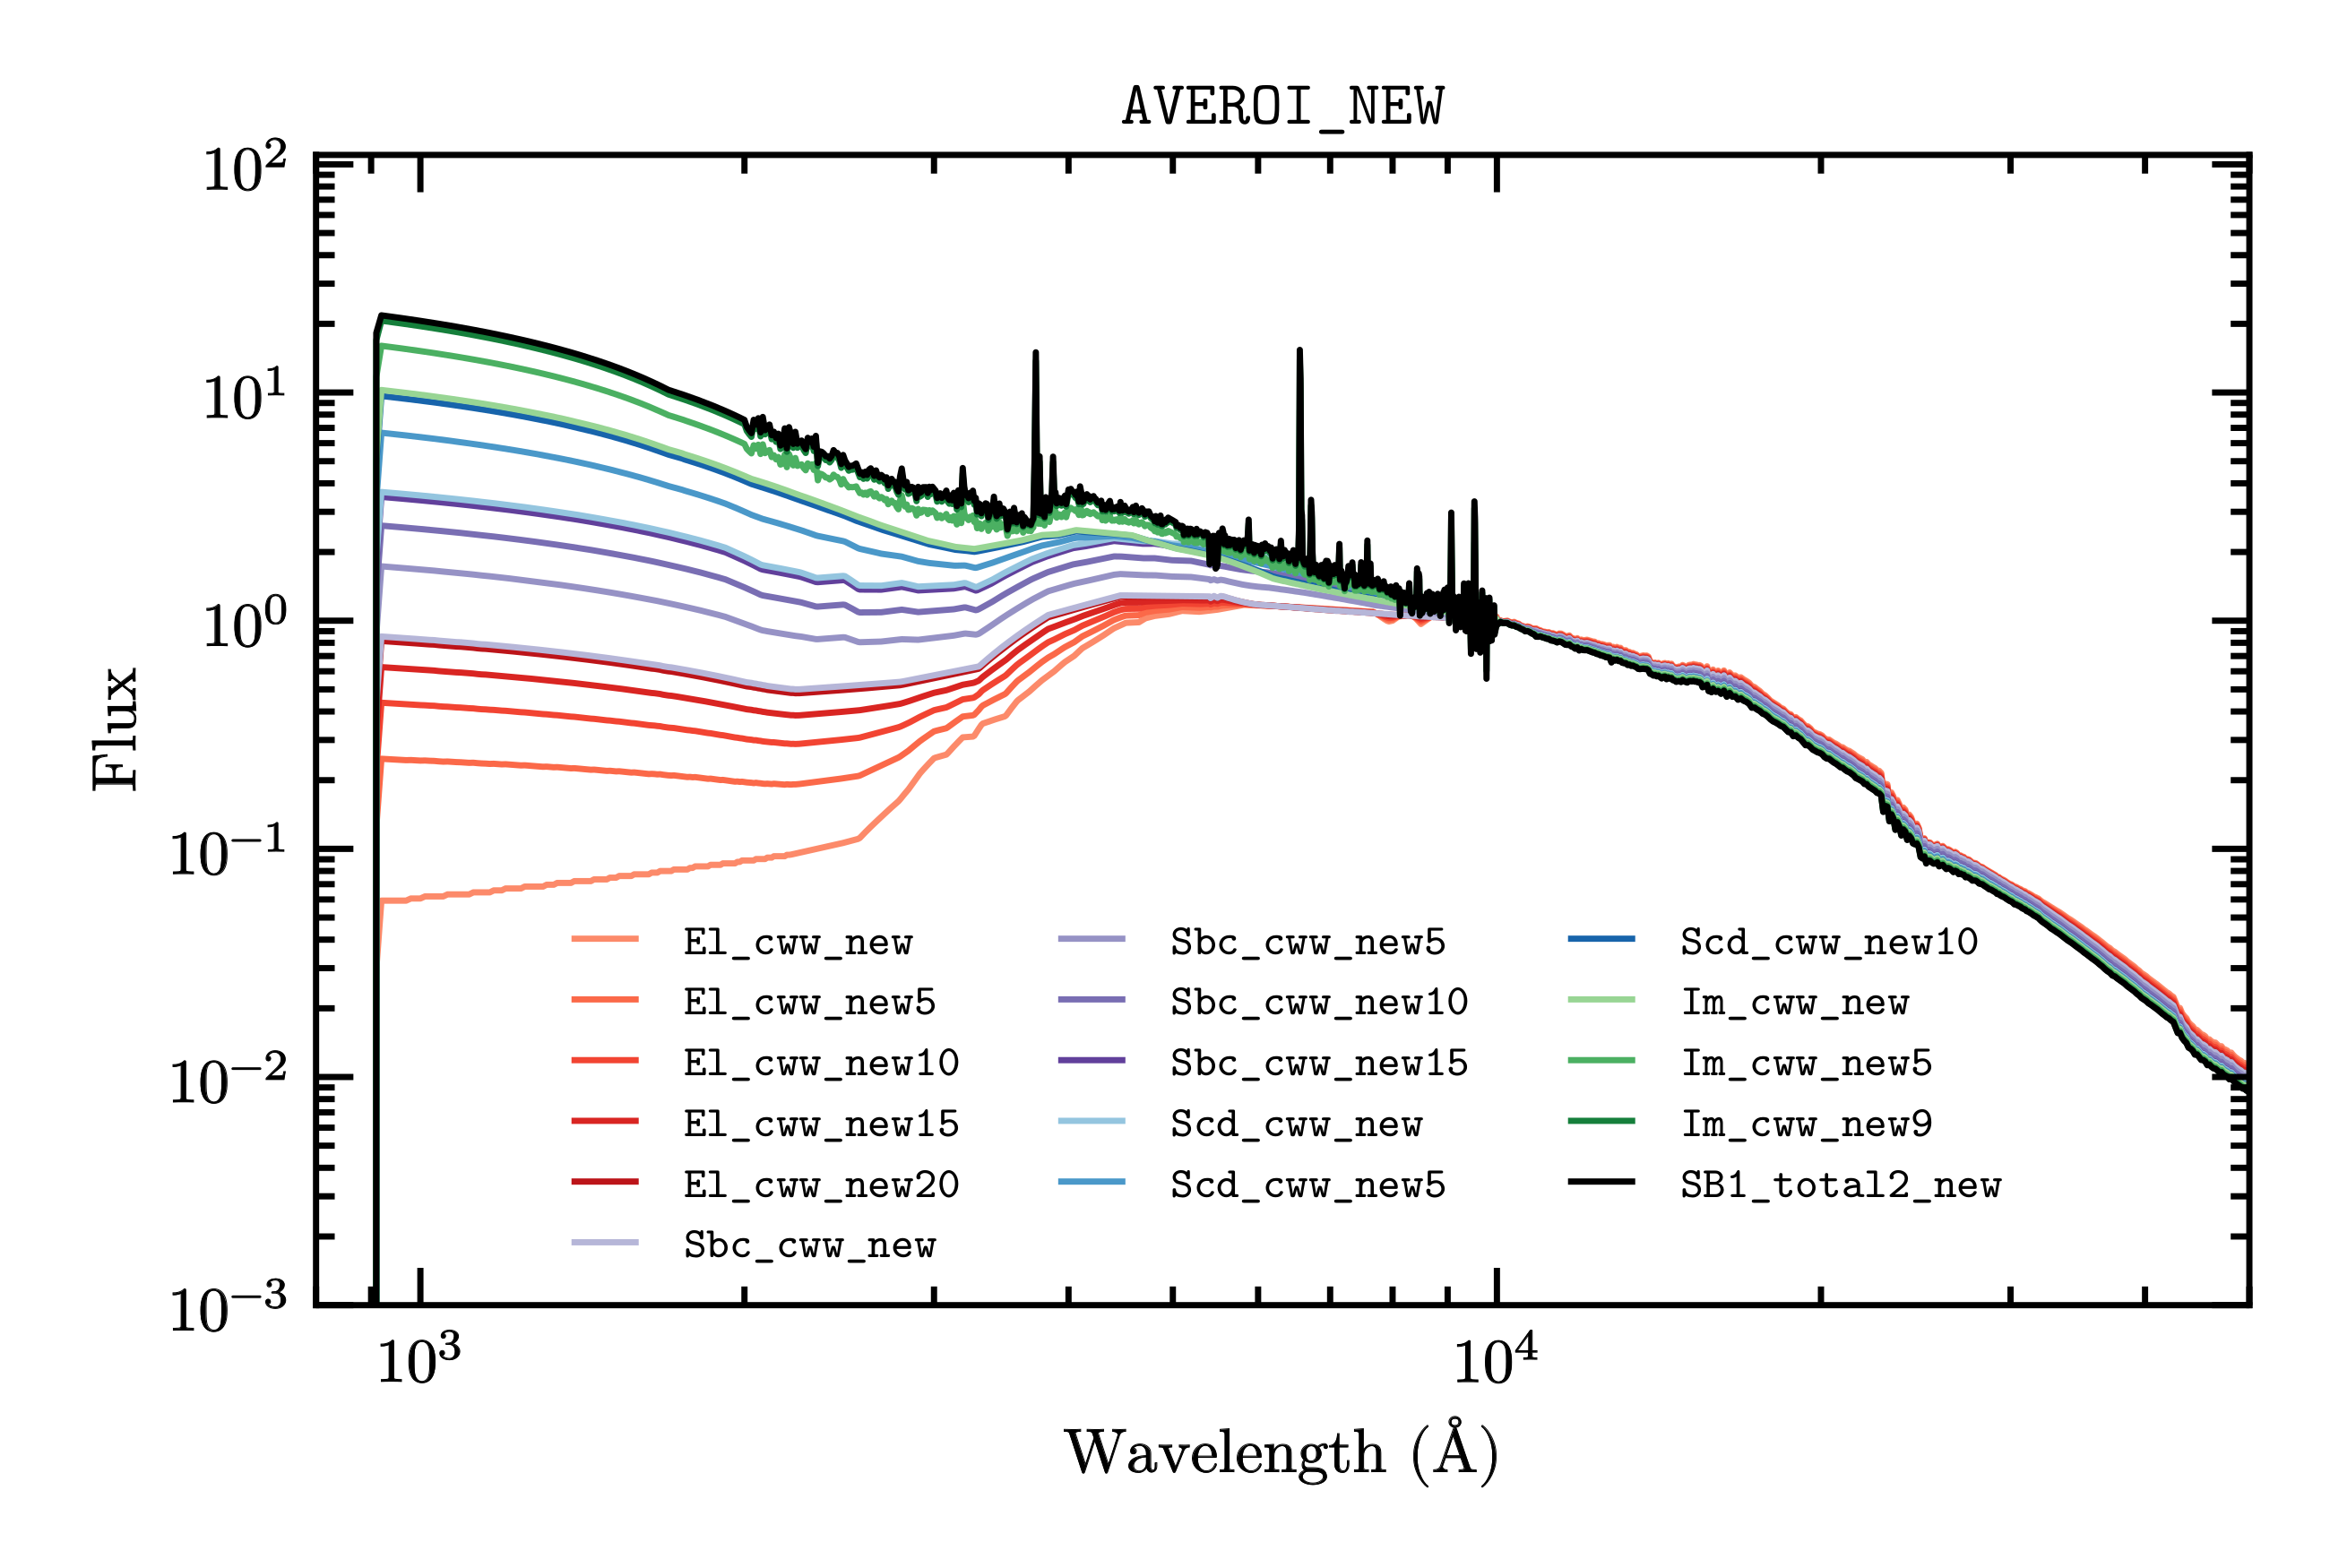
\includegraphics[clip, width=0.95\textwidth]{lephare_template_plots_averoin.png}}

\subfloat[\label{fig:templates_cosmos}]{
	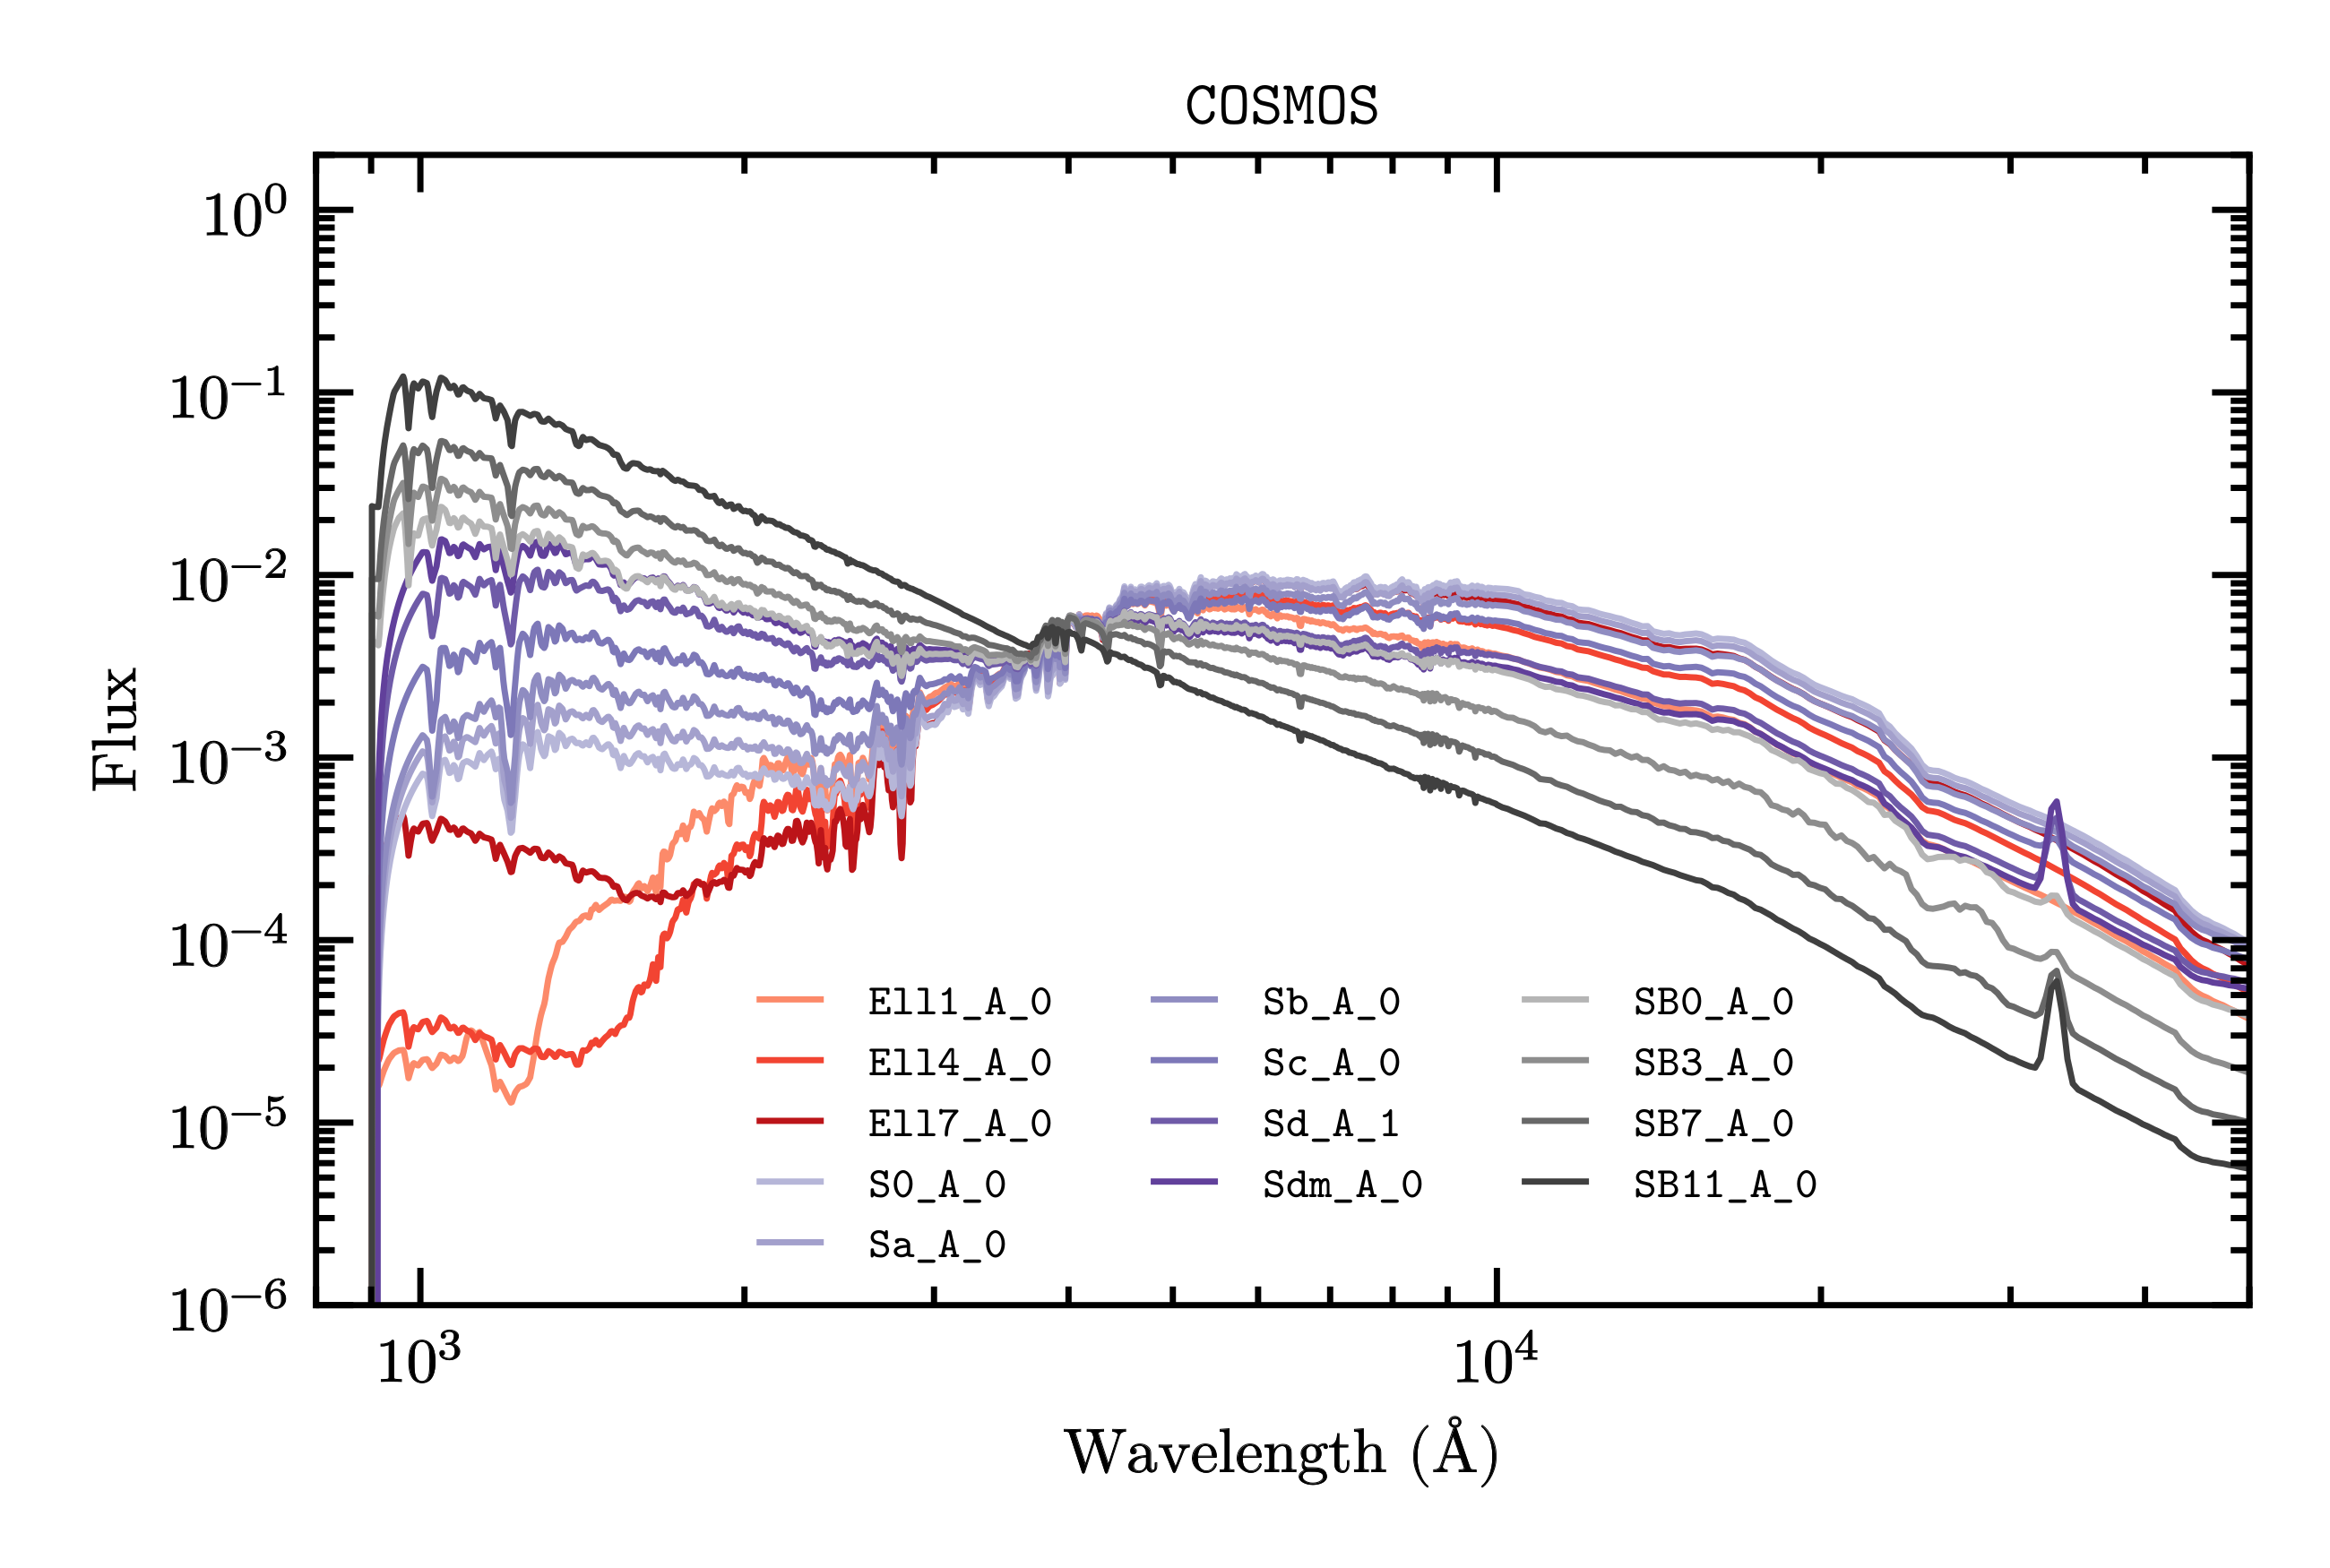
\includegraphics[clip, width=0.95\textwidth]{lephare_template_plots_cosmos.png}}
\caption[Galaxy template SEDs]{Spectra for the two sets of templates used to calculate photometric redshifts for the \DESVIDEO catalogue. The plots display a subset of templates covering a representative fraction of the full template set for \textbf{(a)} the \texttt{AVEROI\_NEW} templates and \textbf{(b)} the \texttt{COSMOS} templates. The names of these templates have been copied directly from the \texttt{LePHARE} installation. Broadly following the Hubble classification scheme for galaxy morphologies, spectra beginning in \texttt{El} or \texttt{Ell} correspond to elliptical galaxies, \texttt{Im} to irregular galaxies, \texttt{SB} to starburst galaxies, \texttt{S0\_A\_D} to a lenticular galaxy, and the other names starting in \texttt{S} to various forms of spirals.}
\label{fig:templates}
\end{figure*}

%among the plethora of photo-z studies

The CWW spectra that form the basis of the \texttt{AVEROI\_NEW} SEDs are a common choice of template among photo-z studies in the literature (e.g. \citealt{1999ApJ...513...34F,1999MNRAS.310..540A}), especially when augmented by starburst templates \citep{1997AJ....113....1S,2006ApJS..162...20B,2006A&A...457..841I}. For the CWW+starburst sets in particular, this choice enjoys strong observational support, as the combination of these templates has been shown to span the range of galaxy properties observed in the Hubble Deep Field over a wide redshift range of $0 < z < 6$ \citep{2000ApJ...536..571B,2002MNRAS.330..889F}. This completeness well into the high-redshift regime suggests that the \texttt{AVEROI\_NEW} templates make a highly appropriate choice for this thesis. \par


 

\subsubsection{\texttt{COSMOS} templates}\label{subsubsection:COSMOS}
The \texttt{COSMOS} template set consists of 31 theoretical SEDs assembled by \cite{2009ApJ...690.1236I} for their photo-z study of the COSMOS field. Nine of these templates were initially created by \cite{2007ApJ...663...81P}, who used the GRASIL code \citep{1998ApJ...509..103S} to generate templates that fitted the observed UV to mid-IR broadband colours of spectroscopically confirmed objects in the VVDS survey \citep{2005A&A...439..845L}. Three of these spectra represent elliptical types and six are spiral types (S0, Sa, Sb, Sc, Sd, Sdm). \cite{2009ApJ...690.1236I} linearly interpolated these nine SEDs to produce 19 templates. Because this collection does not adequately sample the blue end of galaxy colour space, \cite{2009ApJ...690.1236I} generated 12 additional templates using \cite{2003MNRAS.344.1000B} models with starburst ages from 0.03 to 3 Gyr, and extended these beyond 3 $\mu$m using the Sdm \cite{2007ApJ...663...81P} template. Together, all 31 SEDs form the \texttt{COSMOS} template set. Figure \ref{fig:templates_cosmos} shows a subset of these spectra.\par 


Because the \texttt{COSMOS} SEDs have been selected to fit the UV-mid-IR colours of an observed sample, \cite{2009ApJ...690.1236I} claim that they provide a better joining of the UV and mid-IR than  template sets based on the CWW spectra (such as the \texttt{AVEROI\_NEW} templates), which have been extrapolated from the optical theoretically. For this reason, it was deemed of interest to this thesis to test the \texttt{COSMOS} templates as well. Moreover, the \texttt{COSMOS} SEDs have also produced noteworthy observational success. As described above, they were used by \cite{2009ApJ...690.1236I} in the production of their COSMOS 30-band photometric redshift catalogue. Section \ref{subsubsection:multiwavelength_redshifts} previously mentioned
that this catalogue is extremely accurate, with a dispersion of only $\sigma_{\Delta z/ (1+z_{\mathrm{spec}})} =0.007$ (for the brightest $i^{+}_{\mathrm{AB}}<22.5$). \cite{2009ApJ...690.1236I} also demonstrated a 3--5 times improvement in accuracy compared to the previous 16-band COSMOS catalogue \citep{2007ApJS..172..117M} and CFHTLS-Deep results \citep{2006A&A...457..841I}, which were both based on modified versions of the CWW templates. Even though the exceptional accuracy is almost certainly for a large part thanks to the remarkable 30-band coverage, it also corroborates the quality of the \texttt{COSMOS} templates, and suggests that these may be an suitable choice for this thesis. The indicated improvement over CWW+starburst template sets is also interesting, and warrants a comparative investigation with the \texttt{AVEROI\_NEW} performance using the \DESVIDEO dataset.  



\subsection{Stellar and QSO templates}\label{subsection:star_qso_templates}
In addition to galaxy SEDs, \texttt{LePHARE} also determines the best-fit solutions for stellar and quasar (QSO) templates. This feature can be useful, because a comparison of the best-fit $\chi^2$ for each SED type can identify whether the observed colours of a given source are most consistent with a galaxy, a star, or a quasar.
Because stellar sources will have nonsensical photo-zs, they can contaminate photometric redshift catalogues, so it is important to have an effective method for differentiating between stars and galaxies. This task will be addressed in Section \ref{subsection:star_galaxy}, which will describe the process of finding a suitable star-galaxy separation method based on the SED fitting with \texttt{LePHARE}. Rejecting stars and low-redshift QSOs is also be important to the high-redshift galaxy search, so this thesis makes extensive use of the template fitting feature in Chapter \ref{chapter:high_redshift_candidates} as well. \par


To make sure that \texttt{LePHARE} can fit stars accurately, it is important to include a good selection of stellar SEDs. For this reason, it was decided to use the broadest set of stars contained in the default \texttt{LePHARE} installation. This collection consists of a total of 254 templates, composed of 131 empirical star SEDs from \cite{1998PASP..110..863P}, 4 observed white dwarf spectra from \cite{1995AJ....110.1316B}, 18 theoretical models of late-type stars, and a collection of 99 low mass stars and brown dwarfs from \cite{2000ApJ...542..464C}. Having a large selection of SEDs to cover the colours of low mass stars as comprehensively as possible is especially important for this thesis, since low mass stars and brown dwarfs are known to be major contaminants of $z\gtrsim5$ candidates \citep{2009MNRAS.395.2196M,2013AJ....145....4W,2015MNRAS.452.1817B,2016PASA...33...37F}. \par


%LABELLED X IN THE DEFAULT INSTALLATION
The QSO templates used in this thesis are based on models by \cite{2009ApJ...690.1250S}, and are taken from a collection labelled \texttt{QSO\_MARA} in the default \texttt{LePHARE} installation. These models contain  AGN-to-total luminosity ratios of $0.1<L_{\mathrm{AGN}}/L_{\mathrm{tot}}<0.9$, which cover a range of relative contributions to the combined spectrum from AGN or host galaxy emission. \par


\subsection{Extinction}\label{subsection:extinction}
All the templates presented so far are intrinsic SEDs, which do not include the effects of reddening by dust. Instead, \texttt{LePHARE} applies the necessary corrections for dust extinction itself, during the stage where it computes the predicted template magnitudes for Equation \ref{eqn:chi_squared} (see Section \ref{subsubsection:chi_minimisation}). The basic mechanism of dust extinction and its implementation in the code will be briefly described below. \par



Dust grains cause reddening of galaxy spectra by absorbing high energy UV and optical starlight and re-radiating it thermally at IR and submillimeter wavelengths. At a given wavelength $\lambda$ this process causes a shift $A_{\lambda}$ in the observed magnitude compared to the intrinsic (i.e. non-reddened) magnitude:

\begin{equation}
m_{\mathrm{obs}}(\lambda) = m_{\mathrm{int}}(\lambda) + A_{\lambda},\label{eqn:attenuation}
\end{equation}

\noindent where $m_{\mathrm{obs}}$ and $m_{\mathrm{int}}$ are the observed and intrinsic magnitudes respectively, and the shift $A_{\lambda}$ is what is referred to as the extinction (or attenuation). The wavelength dependence of $A_{\lambda}$ is customarily captured by the extinction curve $k(\lambda)$, which is defined as: 


\begin{equation}
k(\lambda) = \frac{A_{\lambda}}{E(B-V)}.\label{eqn:extinction_curve}
\end{equation}

\noindent Here, $E(B-V)$ is a reddening parameter which is equal to the discrepancy between observed and intrinsic $B-V$ colour:
 

\begin{equation}
E(B-V) = (B-V)_{\mathrm{obs}}-(B-V)_{\mathrm{int}}.\label{eqn:eb_v}
\end{equation}

The exact shape of the extinction curve $k(\lambda)$ depends on the content of the interstellar medium, which differs among galaxies.  A functional form has been found for a small number of local objects, notably the Milky Way \citep{1979MNRAS.187P..73S,1976MNRAS.174P..29A}, Large Magellanic Cloud (LMC; \citealt{1986AJ.....92.1068F}), Small Magellanic Cloud (SMC; \citealt{1984A&A...132..389P}; see Figure \ref{fig:extinction}), and starburst galaxies (\citealt{2000ApJ...533..682C}; see Figure \ref{fig:extinction}).  \texttt{LePHARE} allows the user to specify an extinction law and includes the extinction curves from the above studies by default. When applying extinction, the user must also provide a range of values for $E(B-V)$. With these user-specified choices for $k(\lambda)$ and $E(B-V)$, $A_{\lambda}$ can be inferred from Equation \ref{eqn:extinction_curve} and applied to the template SEDs via Equation \ref{eqn:attenuation}, to compute predicted galaxy magnitudes for varying amounts of dust attenuation. \par


For the purpose of this thesis, it was decided to follow the recommended dust extinction procedure for each template set as specified in the \texttt{LePHARE} documentation\footnote{More specifically, in the \texttt{README} files of the default installation.}. Following these instructions, the \texttt{AVEROI\_NEW} templates of star-forming galaxies are attenuated via the  SMC extinction curve. For the \texttt{COSMOS} templates, the SMC law is applied to the redder star-forming galaxies, and the Calzetti law is used for the bluest starburst galaxies. The specific details of the application of dust extinction will be addressed in Section \ref{section:setups}. \par



\begin{figure*}[h]
\centering
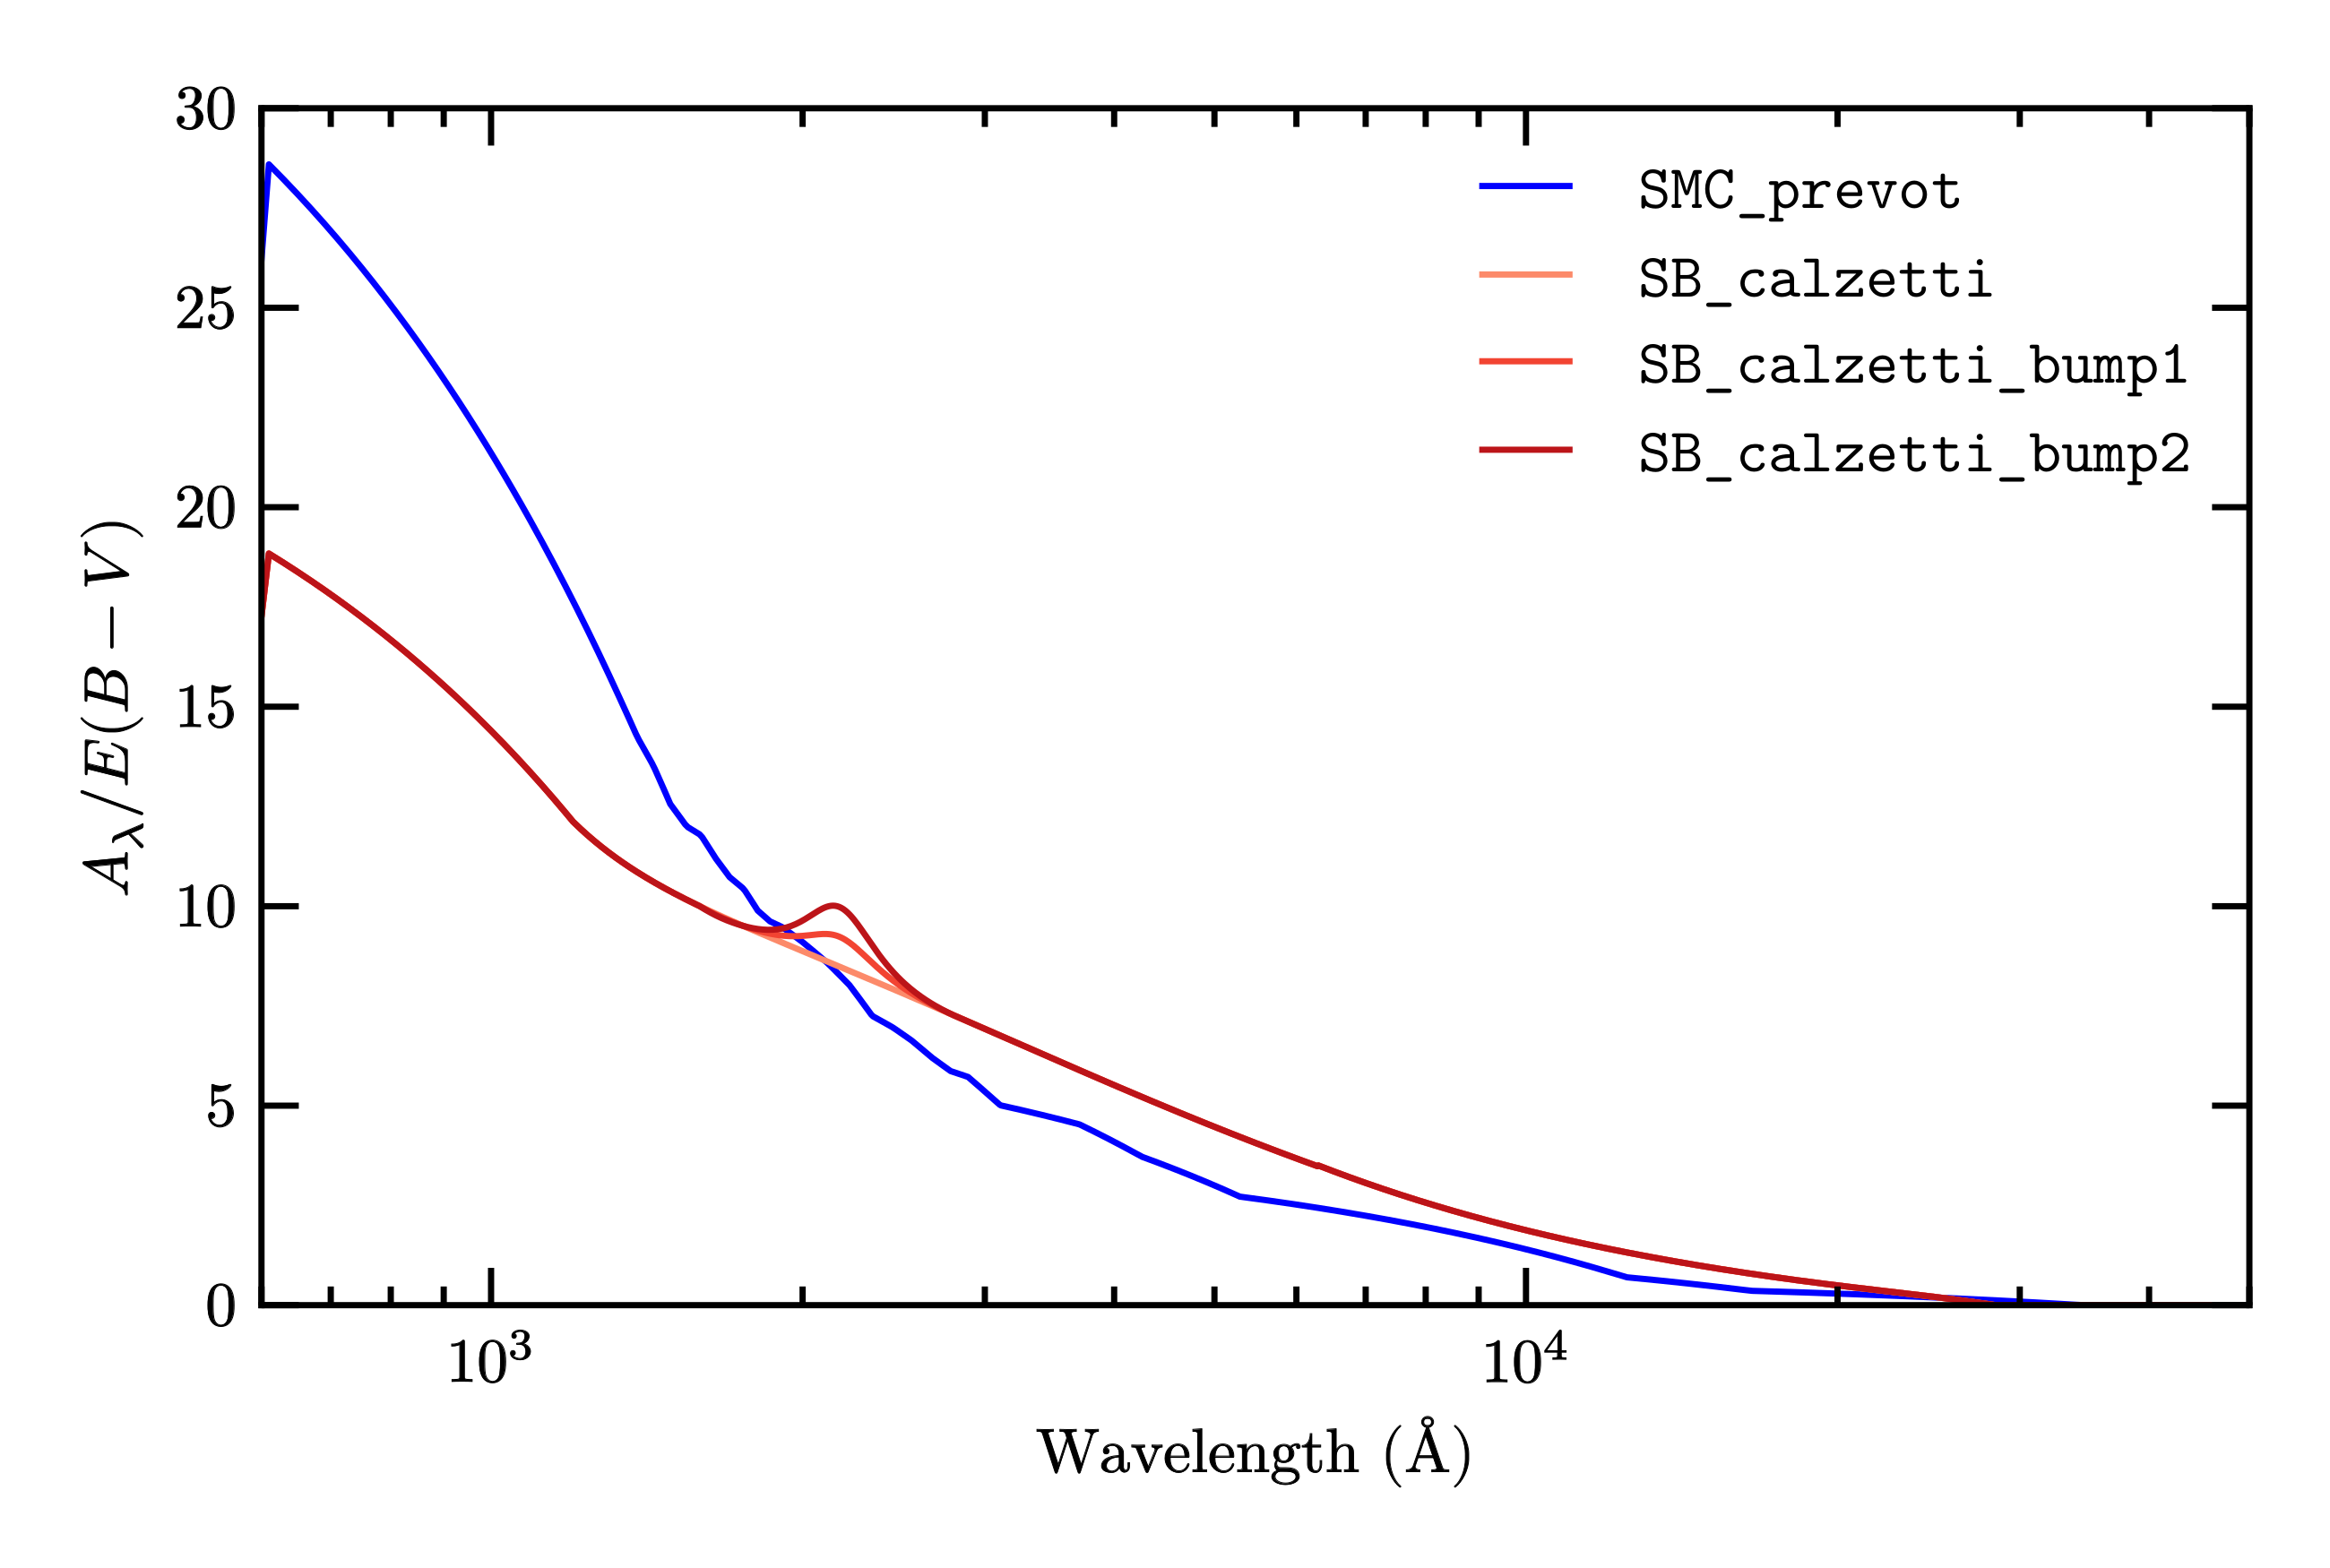
\includegraphics[width=0.95\textwidth]{lephare_extinction_plot.png}
\caption[Dust extinction curves]{Dust extinction curves $k(\lambda) = A_{\lambda} / E(B-V)$ for the SMC \citep{1984A&A...132..389P} and \cite{2000ApJ...533..682C} attenuation laws as included in the default \texttt{LePHARE} installation. There are three available options for the \cite{2000ApJ...533..682C} law, which have differing strengths of the \SI{2175}{\angstrom} bump (see e.g. \citealt{1965ApJ...142.1683S,1994ApJ...422..176M,2011ApJ...733...91X} for more information on this feature).}
\label{fig:extinction}
\end{figure*}


\subsection{Emission lines}\label{subsection:emission_lines}
To ensure that predicted template magnitudes are maximally accurate, it is important to consider the effect of emission lines.  \cite{2009ApJ...690.1236I} argue that strong emission lines can cause notable changes in colour even in broadband filters (up to $\sim0.15$ mag), and that for accurate photometric redshifts, emission lines must therefore be taken into account. \par

There is an option within \texttt{LePHARE} to add Ly$\alpha$, H$\alpha$, H$\beta$, [$\mathrm{O_{II}}$], and [$\mathrm{O_{III}}$] emission lines to the galaxy templates. This feature has been implemented via a process described in \cite{2009ApJ...690.1236I}, which infers the emission line strengths from template UV fluxes. Via a relation from \cite{1998ARA&A..36..189K}, the UV luminosity is firstly used to estimate the global star formation rate (SFR):

%I GOT UP TO HERE. UNITS!!!!!!

\begin{equation}
\mathrm{SFR} (M_{\odot}\mathrm{yr^{-1}} ) = 1.4 \times 10^{-28} L_{\nu,\mathrm{UV}} (\mathrm{erg \ s^{-1} \ Hz^{-1}} ),\label{eqn:kennicut}
\end{equation} 

\noindent which can be related to the [$\mathrm{O_{II}}$] emission line luminosity via:

\begin{equation}
\mathrm{SFR} (M_{\odot}\mathrm{yr^{-1}}) = (1.4 \pm 0.4) \times 10^{-41} L_{[\mathrm{O_{II}}]} (\mathrm{erg \ s^{-1}}).\label{eqn:sfr_oii}
\end{equation}

Putting Equation \ref{eqn:kennicut} and \ref{eqn:sfr_oii} together, and converting luminosity to flux or magnitude, \cite{2009ApJ...690.1236I} obtain:


\begin{equation}
\log{ \left\{ F_{[\mathrm{O_{II}}]}(10^{-17}\mathrm{erg \ s^{-1} cm^2}) \right\} } = -0.1 \times M_{\mathrm{UV}} +10.65 -\frac{DM(z)}{2.5},
\end{equation}

\noindent where $F_{[\mathrm{O_{II}}]}$ is the [$\mathrm{O_{II}}$] line flux, $DM(z)$ is the distance modulus, and $M_{UV}$ is the UV absolute magnitude measured at \SI{2300}{\angstrom} from the (dust-corrected) template SEDs. Because \texttt{LePHARE} can directly measure the latter two quantities, it is able to measure the value of $F_{[\mathrm{O_{II}}]}$ for each (redshifted) template. It then estimates the other emission lines from their intrinsic, unextincted flux ratios with [$\mathrm{O_{II}}$]: $[\mathrm{O_{III}/O_{II}}]=0.36$, $[\mathrm{H}\beta/\mathrm{O_{II}}] = 0.61$, $[\mathrm{H}_{\alpha}/\mathrm{O_{II}}] =1.77$, and $[\mathrm{H}_{\alpha}/\mathrm{O_{II}}] = 2$ \citep{1985ApJS...57....1M,2006ApJ...642..775M,2005MNRAS.362.1143M,1998ARA&A..36..189K}. To obtain the final line strengths, these values are corrected with the appropriate attenuation. At the end, the code adds all the emission lines to the desired predicted magnitudes for the template fitting in \ref{eqn:chi_squared}. It only applies emission lines to templates with a dust free colour bluer than $(NUV-r)_{\mathrm{ABS}} \leq 4$. \par


\section{Photometric redshift configurations}\label{section:setups}
Now the proposed photometric redshift code and template SEDs have been presented, the next step is to introduce the input details for the code. The previous few sections have mentioned several options and parameters in \texttt{LePHARE} that must be specified by the user. The values of these, and various other required inputs, can be provided in configuration files. Throughout this thesis, a particular configuration is referred to as a `setup'. For the \DESVIDEO dataset, a number of setups with different parameters have been tested and compared in terms of their photometric redshift performance, which is assessed by comparing the photo-zs for spectroscopically confirmed galaxies to their measured spectroscopic redshifts. The current section will introduce all these different test configurations.  Afterwards, Section \ref{section:photoz_computation} will then describe the process of computing the photo-zs and various performance assessment measures, which will be analysed in detail in Section \ref{section:photoz_discussion}. \par

 
The photo-z tests have been conducted on the spectroscopic \DESVIDEO subsample only (see Section \ref{subsection:spectra}). The objective is to find the optimal configuration (judged primarily by high-redshift performance) for both the \texttt{AVEROI\_NEW} and \texttt{COSMOS} SEDs, previously introduced in Section \ref{subsection:galaxy_templates}.  The end of this chapter will describe how these setups are used to compute photometric redshifts for the full \DESVIDEO catalogue. There are several reasons for studying two sets of templates in detail. Firstly, computing photo-zs with several template sets makes the \DESVIDEO catalogue more useful as a general resource, as future users will be able to choose which template set is best suited to their particular research. Secondly, the discussion in Section \ref{subsubsection:COSMOS} offered some indications that the \texttt{COSMOS} templates might provide more accurate photo-zs than the \texttt{AVEROI\_NEW} SEDs, which suggests that it is interesting to use the \DESVIDEO data to compare their performance in detail. Thirdly, as one of the aims of this thesis is to perform a precise investigation of how the setup choice impacts photo-zs, the use of different templates provides a better template-independent means of assessing the effect of each configuration parameter.\par


\subsection{The \texttt{default} configurations}\label{subsection:default}
A first attempt at a suitable setup for either template set was constructed by the author, based on a configuration created by \cite{2013MNRAS.428.1281J} for a very similar dataset, and on findings by previous studies. These two setups are subsequently referred to as `\texttt{default}', and the corresponding configuration file for the \texttt{AVEROI\_NEW} templates is shown in full in Appendix \ref{appendix:config_lephare}. \par


\subsubsection{Templates}
The first \texttt{default} input file uses the \texttt{AVEROI\_NEW} templates. To recap, Section \ref{subsubsection:AVEROI_NEW} mentioned that these SEDs were chosen based on the consideration that similar CWW+starburst template combinations have been successful in  many photo-z studies, and that they have been shown to represent galaxies all the way out to $z\sim6$. Following recommendations in the \texttt{LePHARE} documentation, the SMC extinction curve (see Figure \ref{fig:extinction}) is applied to all Scd, irregular (Im in Figure \ref{fig:templates_averoin}) and starburst (SB in Figure \ref{fig:templates_averoin}) spectral types, with $E(B-V)$ values of 0.0, 0.05, 0.1, 0.15, 0.2, 0.3, 0.4, 0.5, 0.7, 1.0. This range is larger than the recommended values listed in the \texttt{README} file of the \texttt{LePHARE} installation, which instead suggests a maximum permitted value of $E(B-V)=0.3$. The higher \texttt{default} maximum was chosen in order to capture very red dusty galaxies, which can contaminate samples of high-redshift candidates (however, the original recommendation of $E(B-V)\leq0.3$ will also be tested via an alternative configuration presented shortly in Section \ref{subsection:alternative_setups}). Finally, the \texttt{AVEROI\_NEW default} configuration adds emission lines to the templates, on the basis that \cite{2009ApJ...690.1236I} claimed that this improves the photometric redshifts (see Section \ref{subsection:emission_lines}).\par

The second \texttt{default} setup uses the \texttt{COSMOS} SEDs. Earlier on, Section \ref{subsubsection:COSMOS} suggested that these templates may be a suitable choice based on previous observational success. In the \texttt{COSMOS default} configuration, dust extinction is applied with values of $E(B-V) = 0.0, 0.1, 0.2, 0.3, 0.4, 0.5$. The Calzetti extinction law (see Figure \ref{fig:extinction}) is applied to the SB3 galaxy type and all bluer types (the reader is referred to Figure \ref{fig:templates_cosmos} for a clarification of the \texttt{COSMOS} spectral types), and the SMC law (see Figure \ref{fig:extinction}) is applied to all types redder than SB3 (including SB3). No extinction is applied to galaxies redder than Sb. The Calzetti law is applied three times, once for each of the three strengths of the \SI{2175}{\angstrom} bump in Figure \ref{fig:extinction}. All the above decisions directly follow the recommendations in the \texttt{LePHARE} installation, which are also covered in \cite{2009ApJ...690.1236I}. For the same reasons listed for the \texttt{AVEROI\_NEW} templates, emission lines are enabled for the \texttt{COSMOS} \texttt{default} configuration.\par 



\subsubsection{Photometric redshift code options for the \texttt{default} configurations}\label{subsubsection:photoz_options_default}
Sections \ref{subsection:prior} and \ref{subsection:adaptive_offsets} introduced two options in \texttt{LePHARE} designed to aid in the redshift estimations. The \texttt{default} setups each use both these features, discussed below and implemented as described.\par


\paragraph{$N(z)$ prior} The \texttt{default} configurations both enable the option to apply a luminosity prior $N(z)$, described in Section \ref{subsection:prior}. The discussion there described how the use of a prior is likely to be helpful for this thesis, as it has been shown to reduce outliers. As mentioned, the $N(z)$ prior in \texttt{LePHARE} refers to the $B-I$ colour of objects in the VVDS. While the DES observations naturally do not include $B$-band data, \cite{2014MNRAS.445.1482S} have demonstrated that DES $g-i$ colour is a reasonable substitute, so the \texttt{default} configurations use these two filters as input for the prior. \par



\paragraph{Adaptive offsets}Section \ref{subsection:adaptive_offsets} presented several reasons why the inclusion of adaptive offsets, which calibrate zero-point offsets via spectroscopic redshifts, might be beneficial for the \DESVIDEO catalogue. In particular, the ability to incorporate aperture corrections, and the capacity to compensate for uncertainties in the photometric zero-point calibration are considered especially important to this thesis. With these arguments in mind, it was decided to activate this option in the \texttt{default} configurations. \par

Inconveniently, a quick first attempt at calculating suitable adaptive offsets for each \DESVIDEO tile revealed that the offsets determined by \texttt{LePHARE} vary considerably from tile to tile. This is not unexpected --- differences in imaging quality and cosmic variance can cause such an effect in several ways. For starters, the seeing fluctuates across tiles, which leads to different compensation for aperture corrections. Secondly, due to the varying depth and cosmic variance, the galaxy populations observed in each tile are different as well. Because of the effect that template incompleteness can have on the adaptive offset values, differences in spectral types can lead to disparity in the offsets. \par

The reasoning above implies that the adaptive offsets would be most accurate when computed on a DES tile-to-tile basis. Unfortunately, some DES tiles contain an insufficient number of spectroscopic redshifts to make the calculated values statistically sound (e.g. there exist 19 DES tiles with <100 spectra). However, each of the eight VIDEO tiles does include a sizeable number (>1000) of spectra. It was therefore decided to compute the adaptive offsets individually for each VIDEO tile. This ensures that the offsets are based on VIDEO imaging with constant limiting magnitudes. There are still depth differences among each of the DES co-adds covering a given VIDEO tile, but this variation is generally smaller than the DES variation over the full footprint (see Figures \ref{fig:depth_es1}, \ref{fig:depth_xmm}, and \ref{fig:depth_cdfs}). Therefore, the proposed strategy method provides a good balance, allowing the adaptive offsets to capture most of the depth variation, while also ensuring that they are based on a statistically sound number of spectra. \par

Because the uncertainties in the adaptive offsets computed by \texttt{LePHARE} are not better than \SI{0.01}{\mag} \citep{2009ApJ...690.1236I}, a value of 0.01 is added in quadrature to the apparent magnitude errors in the input photometry\footnote{This is taken care of by specifying a value of \SI{0.01}{\mag} for the \texttt{ERR\_SCALE} parameter, which leads \texttt{LePHARE} to increase the errors automatically.}. 

\subsubsection{Input photometry for the \texttt{default} configurations}\label{subsubsection:input_phot_default}
Naturally, in order to be able to compute photometric redshifts, \texttt{LePHARE} requires the user to supply input photometry. For the \texttt{default} setups, these input files consist of fluxes in all the \DESVIDEO $grizZYJHK_{s}$-bands (note that this excludes the DES $Y$-band, which is too shallow compared to the other bands to be useful for the photo-zs in this thesis), measured in a fixed \SI{1.95}{\arcsec} diameter aperture. The choice for fixed-size aperture fluxes over auto photometry was mirrored on similar studies in the literature (e.g. \citealt{2009ApJ...701.1839M,2013MNRAS.428.1281J,2012MNRAS.426.2772B,2014MNRAS.440.2810B}). The relatively small \SI{1.95}{\arcsec} size was chosen because high-redshift candidates are expected to be faint, and measuring fluxes over too large an aperture compromises the signal-to-noise for faint sources \citep{2019NatAs...3..212S}. The aperture diameter is therefore designed to be not much larger than the expected spatial extent of $z\gtrsim5$ galaxies. In previous ground-based surveys with similar seeing, galaxy sizes around $z\sim6$ have generally been dominated by the seeing \citep{2013AJ....145....4W,2014MNRAS.440.2810B,2015MNRAS.452.1817B}. Given that the DES and VIDEO FWHM is around $\sim\SI{1}{\arcsec}$, \SI{1.95}{\arcsec} apertures are expected to enclose the majority of galaxy flux, while also being small enough to minimise photometric noise. A comparable \SI{2}{\arcsec} diameter has also been used by previous studies with similar datasets \citep{2013MNRAS.428.1281J,2012MNRAS.426.2772B}, and has been shown to deliver good results at low redshifts as well \citep{2009ApJ...701.1839M,2013MNRAS.428.1281J}. \par 


\subsection{Alternative configurations}\label{subsection:alternative_setups}
To investigate the effect of different input parameters on the photo-zs, the performance of the \texttt{default} setup for both template sets is compared to other possible configurations. Each of these rival setups is identical to the \texttt{default} version with the exception of one factor. This section presents all the alternative setups for this investigation, alongside a clarification of which parameters have been changed. \par

{\vspace{1em plus 0.2em minus 0.1em}}
\textit{The configurations for the following four setups are template dependent, and are defined individually for each template set:} \par

\subparagraph{\texttt{AVEROI\_NEW less\_ext}} This setup uses the original extinction recommendation found in the \texttt{README} file for the \texttt{AVEROI\_NEW} templates in the \texttt{LePHARE} installation. These values equal $E(B-V)=0.0,0.05,0.10,0.15,0.20,0.25,0.30$. The aim of this setup is to investigate whether this lower extinction range is sufficient to produce accurate photo-zs, by testing whether it performs as well as (or better than) the wider range of up to $E(B-V)=1.0$ used in the \texttt{default} setup. 

\subparagraph{\texttt{AVEROI\_NEW more\_ext}} As emphasised throughout this chapter, a priority for the \DESVIDEO photo-zs is optimal performance at $z\gtrsim5$. Very red dusty galaxies are a known contaminant at these redshifts \citep{2016PASA...33...37F}, because their extremely red colours replicate those of true high-redshift sources in some filters. The \texttt{more\_ext} setup tests whether maximally reducing contamination at high redshifts requires even higher extinction than the \texttt{default} values, in order to capture adequately the colours of any extremely red low-redshift interlopers. The permitted extinction range in the \texttt{more\_ext} setup equals $E(B-V) = 0.0, 0.05, 0.1, 0.15, 0.2, 0.3, 0.4, 0.5, 0.7, 1.0, 1.3, 1.6, 2.0$. 

\subparagraph{\texttt{COSMOS} \texttt{ext}, \texttt{more\_ext}} The \texttt{default} setup for the \texttt{COSMOS} templates uses extinction values of up to $E(B-V)=0.5$. For the same reasons as for the \texttt{AVEROI\_NEW more\_ext} setup above, the \texttt{COSMOS} \texttt{ext} and \texttt{more\_ext} configurations test whether a larger amount of reddening is required for optimal (high-redshift) results. The permitted extinction values are $E(B-V)=0.0,\allowbreak 0.1,\allowbreak 0.2,\allowbreak 0.3,\allowbreak 0.4,\allowbreak 0.5,\allowbreak 0.7,\allowbreak 1.0$ for the \texttt{ext} setup, and $E(B-V)=0.0,\allowbreak 0.1,\allowbreak 0.2,\allowbreak 0.3,\allowbreak 0.4,\allowbreak 0.5,\allowbreak 0.7,\allowbreak 1.0,\allowbreak 1.3,\allowbreak 1.6,\allowbreak 2.0$ for the \texttt{more\_ext} configuration. \par

{\vspace{1.2em plus 0.2em minus 0.1em}}\textit{The remainder of the alternative setups are the same for both the \textup{\texttt{AVEROI\_NEW}} and \textup{\texttt{COSMOS}} template sets (i.e. each configuration contains the same change to the respective \textup{\texttt{default}} setups).} \par


\subparagraph{\texttt{no\_emlines}} To evaluate whether the photometric redshift accuracy improves by adding emission lines to the templates (as claimed by \citealt{2009ApJ...690.1236I}), emission lines are turned off in the \texttt{no\_emlines} setups.

\subparagraph{\texttt{no\_adapt}} The use of adaptive offsets is disabled in the  \texttt{no\_adapt} setups, in order to assess how the offsets affect the photo-z results. 

\subparagraph{\texttt{no\_prior}} Due to fact that known distributions of galaxies are heavily skewed towards low redshifts, including an $N(z)$ prior will inherently bias photo-z estimates against high-redshift solutions \citep{2000ApJ...536..571B}. This could potentially remove some genuine high-redshift galaxies from any resulting $z\gtrsim5$ sample. It is therefore interesting to investigate whether it is possible to avoid using a prior, while still maintaining a manageable level of high-redshift contamination by low-redshift interlopers. Interestingly, several results in the literature indicate that the inclusion of near-infrared photometry may help to break the colour-redshift degeneracies that can lead to those contaminating catastrophic outliers \citep{2000ApJ...536..571B,2006A&A...457..841I}. To investigate whether the \DESVIDEO catalogue does in fact contain enough photometric data to permit not using a prior, the \texttt{no\_prior} configurations test the photo-z performance without the use of an $N(z)$ prior. 
 

\subparagraph{\texttt{auto}} As mentioned previously in Section \ref{subsection:default}, it is common in the literature to use aperture magnitudes as input photometry, and the \texttt{default} configurations follow this custom. To test the validity of this assumption, the \texttt{auto} setups use an input catalogue based on auto fluxes instead. 



\subparagraph{\texttt{des}, \texttt{des\_auto}} While the default setups use data from all nine $grizZYJHK_{s}$ \DESVIDEO bands, the \texttt{des} and \texttt{des\_auto} configurations only include flux measurements from the DES $griz$ filters, using aperture and auto photometry respectively. By assessing the photo-z performance without the VIDEO data, these setups can probe the extent to which near-IR coverage improves the photometric redshifts.



\section{Configuration testing}\label{section:photoz_computation}
\subsection{Photometric redshift computation method}\label{subsection:photoz_computation_method}
The next stage in the investigation aims to quantify which is the most suitable configuration for the \DESVIDEO catalogue. To this end, photometric redshifts have been computed for the subset of galaxies with spectroscopic redshifts, using all of the 18 configurations introduced in the previous section (9 for each template set). The redshifts have been obtained via a procedure with several stages, which ensure that the resulting photo-zs are as reliable as possible. This algorithm consists of the following steps: 

\begin{enumerate}
    \item Firstly, the list of sources with spectroscopic redshifts (see Section \ref{subsection:spectra}) is combined with the \DESVIDEO dataset. To do this, the spectra are matched within a \SI{1}{\arcsec} radius to the \DESVIDEO tables from step 7 of the assembly pipeline in Section \ref{subsection:catalog_production}, i.e. the photometric catalogues for each combination of overlapping DES and VIDEO tiles. At this stage, the objective of the spectroscopic redshifts is to calibrate adaptive offsets. Therefore, in order to make sure that the input data for these offsets is maximally reliable, the algorithm removes spectroscopic objects with a bad \texttt{FLAGS\_WEIGHT} value in any DES or VIDEO band. This criterion also applies to the DES $Y$-band, which is not used in any subsequent photo-z computations. The reason why it is nonetheless included here relates to the need for reliable input fluxes. As described in Section \ref{subsubsection:data_quality}, the \texttt{FLAGS\_WEIGHT} value in a given band is non-zero if the object overlaps a region with bad data or no data in that filter. In the case of the DES data, these bad regions include chip gaps. The images in all DES bands are severely more noisy in the vicinity of these gaps, but the DESDM catalogue uncertainties have not been suitably adjusted to account for this, which results in unreliable photometry around those regions. Because the weight maps in the five $grizY$-bands have slightly different widths for the chip gaps, using the \texttt{FLAGS\_WEIGHT} parameter in all bands ensures the exclusion of as many objects as possible in the noisy border regions. 
    
    %\footnote{}
    
    %I GOT UP TO HERE
    
    \item For each VIDEO tile, the algorithm then merges the spectroscopic catalogues from step 1 together for all the \DESVIDEO tiles that overlap that VIDEO tile. In the merging process, any duplicate spectra from overlapping DES tiles are removed, so that the combined catalogues include each spectrum only once per VIDEO tile. The duplicates are removed by rejecting any objects that do not exist within the non-duplicate version of the DESDM catalogues (assembled previously by the author as described in Section \ref{subsubsection:duplicates}). 
    
    %THIS IS BECAUSE OF THE ADAPTIVE OFFSETS
    \item To calculate photometric redshifts, \texttt{LePHARE} is run individually on each of the VIDEO tiles, using all of the 18 setups introduced in Section \ref{section:setups} (9 for each template set). The input contains photometry and spectroscopic redshifts from the catalogues in step 2, and the output consists of the standard \texttt{LePHARE} output, which includes photometric redshifts for all sources, as well as adaptive offsets (for the configurations where they were enabled).  Running \texttt{LePHARE} in the above way automatically achieves the goal previously laid out in Section \ref{subsubsection:photoz_options_default}, of calibrating the adaptive offsets for each VIDEO tile individually. 
    
    \item For each configuration, the \texttt{LePHARE} results from all eight VIDEO tiles are then merged together. To achieve this, the algorithm stacks the eight output files from step 3. The objective of these merged datasets is to enable a statistical analysis of the photo-z performance for each setup (which will be described later in Section \ref{subsection:accuracy_metrics}). Initially, the simple stacked catalogues contain duplicates from the overlapping regions between tiles. While these duplicate objects were needed in the earlier steps to make sure that the adaptive offsets are based on a maximal number of spectra, they introduce bias in the statistics. Duplicates are therefore removed; when a single DES object is covered by multiple VIDEO tiles, the algorithm retains the data from the highest ranking VIDEO tile. The author determined this ranking from Table \ref{table:error_agreement}, based on the depths and available bands. In order of descending priority, the order is: (es1-north, es1-south) for the ELAIS-S1, (xmm3, xmm2, xmm1) for the XMM-LSS and (cdfs1, cdfs2, cdfs3) for the CDF-S. The final product is a series of 18 photo-z catalogues (one for each configuration), where each spectrum is included only once. 
    
\end{enumerate}

After the above algorithm was applied to the \DESVIDEO dataset, the resulting 18 photo-z catalogues each contain a total of \num{35596} sources with spectrocopic and photometric redshifts. \par


\subsection{Accuracy metrics for assessing photo-z performance}\label{subsection:accuracy_metrics}
The redshift catalogues from the previous section can be used to assess the photo-z performance of each configuration. To do so, this thesis uses eight accuracy metrics, largely following \cite{2014MNRAS.445.1482S}.  In this framework, the individual bias (i.e. the photometric-to-spectroscopic discrepancy) for each object $i$ is defined as $\Delta z_{i} = z_{\mathrm{phot},i}-z_{\mathrm{spec},i}$, and $N$ represents the total number of objects used in the estimation of the statistics. Using these notations, eight statistical measures have been defined to capture various aspects of the photo-z distribution:



\begin{enumerate}[label=(\roman*)]
\item \textbf{Bias}. Two metrics capture the average bias. The first of these is the mean bias $\overbar{\Delta z}$, which is defined as follows:
\begin{equation}
\overbar{\Delta z} = \frac{1}{N} \sum^{N}_{i} \Delta z_{i}. \label{eqn:bias}
\end{equation}
  
Secondly, the median bias $\Delta z_{50}$ corresponds to the median of the $\Delta z$ distribution, defined as the (interpolated) middle value of an ordered list of $\Delta z_{i}$ values. In other words, the median is the value of $\Delta z$ that satisfies the following equation:

\begin{equation}
 P_{50} \equiv P(\Delta z \leq \Delta z_{50}) = \frac{1}{2}. \label{eqn:median}
\end{equation}
 
\item \textbf{Scatter}. The scatter is measured by two separate statistics, corresponding to the two bias metrics defined above. Firstly, there is the standard deviation $\sigma$ of the mean bias $\overbar{\Delta z}$, which is expressed as: 

 \begin{equation}
 \sigma = \sqrt{\frac{1}{N} \sum^{N}_{i} (\Delta z_{i} - \overbar{\Delta z})}.
 \end{equation}

The second statistic measures the 68 percentile width $\sigma_{68}$ of the $\Delta z$ distribution about the median bias $\Delta z_{50}$; in other words, $\Delta z_{50} \pm \sigma_{68}$ encloses 68\% of the $\Delta z$ distribution:

\begin{equation}
\sigma_{68} = \frac{1}{2} (\Delta z_{84} - \Delta z_{16}),
\end{equation}
 
\noindent where $\Delta z_{84}$ and $\Delta z_{16}$ are defined analogously to $\Delta z_{50}$ in Equation \ref{eqn:median}. \par


In the specific case where the values of $\Delta z_i$ are normally distributed, it is the case that $\sigma = \sigma_{68}$. However, in general the bias distribution is not Gaussian, and $\sigma_{68}$ captures the scatter in the core of the $\Delta z$ distribution  $\sigma$ is more sensitive to the tails.\par  

\item \textbf{Outliers}. The number of objects with significantly bad photo-z estimates is quantified in the outlier fractions. The $2\sigma$ outlier fraction $f_{2\sigma}$, which measures the fraction of objects more than $2\sigma$ away from the mean, can be written as: 
  \begin{equation}
  f_{2\sigma} = \frac{1}{N}\sum^{N}_{i}{W_{2,i}},
  \end{equation}
where
  \[
  W_{2,i} =
  \begin{cases}
  1, & \text{if } \left| \Delta z_{i} - \overbar{\Delta z} \right| > 2 \sigma \\
  0, & \text{if } \left| \Delta z_{i} - \overbar{\Delta z} \right| \leq 2 \sigma 
  \end{cases}.
  \]

Similarly, the $3\sigma$ outlier fraction $f_{3\sigma}$ is expressed as follows:
  \begin{equation}
  f_{3\sigma} = \frac{1}{N}\sum^{N}_{i}{W_{3,i}}, \label{eqn:frac3}
  \end{equation}
where
  \[
  W_{3,i} =
  \begin{cases}
  1, & \text{if } \left| \Delta z_{i} - \overbar{\Delta z} \right| > 3 \sigma \\
  0, & \text{if } \left| \Delta z_{i} - \overbar{\Delta z} \right| \leq 3 \sigma 
  \end{cases}.
  \]
  
  \item \textbf{High-redshift performance.} The six numbered equations above, all based on \cite{2014MNRAS.445.1482S}, capture the photo-z accuracy for the full redshift range (within a given configuration). To determine the performance at high redshifts specifically, the author has defined two additional metrics. The first quantity $N_{\mathrm{int}}$ captures the galaxy contamination by counting the number of low-redshift ($z_{\mathrm{spec}}<2.0$) interlopers in a $z_{\mathrm{phot}}>4.0$ sample. It is defined as follows: 
  \begin{equation}
      N_{\mathrm{int}} = \sum^{N}_{i}{W_{\mathrm{int},i}},\label{eqn:N_int}
  \end{equation}
  where
    \[
  W_{\mathrm{int},i} =
  \begin{cases}
  1, & \text{if } z_{\mathrm{phot}}>4.0 \text{ and } z_{\mathrm{spec}}<2.0 \\
  0, & \text{ otherwise} 
  \end{cases}.
  \]
  
  The second high-redshift metric $N_{\mathrm{good}}$ counts the number of actual high-redshift ($z_{\mathrm{spec}}$ > 3.5) objects that are retrieved at high redshift (with $z_{\mathrm{phot}}$ within 0.5 of $z_{\mathrm{spec}}$):
  \begin{equation}
      N_{\mathrm{good}} = \sum^{N}_{i}{W_{\mathrm{good},i}},\label{eqn:N_good}
  \end{equation}
  where
    \[
  W_{\mathrm{good},i} =
  \begin{cases}
  1, & \text{if } z_{\mathrm{spec}}>3.5 \text{ and } \left| z_{\mathrm{spec}} - z_{\mathrm{phot}} \right| < 0.5 \\
  0, & \text{ otherwise} 
  \end{cases}.
  \]  
  The reader may have noticed that the meaning of the phrase `high-redshift' for the two metrics $N_{\mathrm{int}}$ and $N_{\mathrm{good}}$ is slightly different from the general $z\gtrsim5$ definition used throughout this thesis. This is because the spectroscopic subsample does not contain any spectroscopic redshifts above $z_{\mathrm{spec}}=5.0$, and only 11 objects at $z_{\mathrm{spec}}>4.0$. To obtain the closest possible measurement of the $z\gtrsim5$ performance, it is therefore necessary to lower the definition of high redshifts for $N_{\mathrm{good}}$, and to assume that this metric gives an indication of the true accuracy at $z\gtrsim5$. It is emphasised that placing the threshold at $z_{\mathrm{spec}}>3.5$ should avoid $N_{\mathrm{good}}$ being significantly biased by issues with colour-redshift degeneracies from confusion between the Lyman and \SI{4000}{\angstrom} breaks (since a Lyman break between \SI{912}{\angstrom} and \SI{1216}{\angstrom} enters the $g$-band between $z=3.36$ and $z=2.27$ respectively and breaks the degeneracy). Therefore, there ought to be no major issues inherent within the photometric redshift method that implies that the $z_{\mathrm{spec}}>3.5$  performance does not carry over to $z\gtrsim5$. Regarding $N_{\mathrm{int}}$, the $z_{\mathrm{phot}}=4.0$ cutoff is likewise below $z=5.0$, this time to ensure that $N_{\mathrm{int}}$ captures contamination over a slightly wider photo-z range.  When this metric is used to find the best configuration for the $z\gtrsim5$ galaxy search, the $z_{\mathrm{phot}}=4.0$ threshold minimises the potential effect of low-redshift objects around $z_{\mathrm{phot}} \sim 4.5$ scattering into a $z_{\mathrm{phot}}\gtrsim5$ sample. Furthermore, the lower cutoff also ensures consistency with the value used for $N_{\mathrm{good}}$. 
  
  %CHECK THIS, SHORTEN THIS FOR FORMATTING ISSUES, NEED TO CUT OUT LIKE 10 LINES THOUGH
  
\end{enumerate}


\subsection{Results}\label{subsection:photoz_results}

The statistics introduced above have been calculated for all the configurations from Section \ref{section:setups}. Table \ref{table:photoz_test} shows the results, grouped together by template set. For every one of the setups, the distribution of spectroscopic vs photometric redshift is also plotted in Figure \ref{fig:photoz_distribution}. Together, these plots and metrics provide a comprehensive picture of the photo-z performance. Naturally, smaller values for the metrics generally imply better accuracy for all indicators except $N_{\mathrm{good}}$, where a larger value is better (since it indicates that a larger number of $z_{\mathrm{spec}}>3.5$ objects were correctly assigned a high redshift). When considering the performance, one must bear in mind that some metrics are interdependent. Most importantly, the $2\sigma$ and $3\sigma$ outlier fractions $f_{2\sigma}$ and $f_{3\sigma}$ depend on the value of $\sigma$. Because a higher scatter widens the bounds of $f_{2\sigma}$ and $f_{3\sigma}$, lower values for these outlier fractions only indicate a better performance if the scatter $\sigma$ is the same or lower. Lastly, for the purpose of this thesis, only the absolute value of the mean and median bias is important,  because it only matters how much these quantities differ from zero.\par


{\vspace{5em plus 2em minus 5em} \penalty-200}


\begin{table}[hb]
\setlength{\tabcolsep}{0.5em}

\centering
\textsc{Photo-z accuracy for the \texttt{AVEROI\_NEW} templates} \\
\vspace{0.1em}
\footnotesize
\begin{tabular}{lcccccccc}
\toprule\toprule
setup & $\overbar{\Delta z}$ & $\Delta z_{50}$ & $\sigma$ & $\sigma_{68}$ &  $f_{2\sigma}$ & $f_{3\sigma}$ & $N_{\mathrm{int}}$ & $N_{\mathrm{good}}$ \\
\midrule
\texttt{default} & 0.00259 & 0.01675 & 0.47682 & 0.09439 & 0.04335 & 0.02669 & 105 & 23 \\
\texttt{less\_ext} & 0.02224 & 0.01706 & 0.51961 & 0.10407 & 0.04610 & 0.02910 & 120 & 23 \\
\texttt{more\_ext} & 0.00220 & 0.01675 & 0.47683 & 0.09448 & 0.04340 & 0.02677 & 104 & 23 \\
\texttt{no\_emlines} & -0.00112 & 0.01127 & 0.47774 & 0.09221 & 0.04321 & 0.02677 & 109 & 23 \\
\texttt{no\_prior} & 0.01475 & 0.01590 & 0.52508 & 0.09914 & 0.04332 & 0.02641 & 176 & 27 \\
\texttt{no\_adapt} & -0.00260 & 0.01488 & 0.50593 & 0.12308 & 0.04363 & 0.02801 & 119 & 22 \\
\texttt{auto} & -0.01653 & 0.01007 & 0.46644 & 0.10813 & 0.04377 & 0.02641 & 72 & 14 \\
\texttt{des} & -0.00438 & 0.01122 & 0.48223 & 0.17451 & 0.04976 & 0.03113 & 5 & 16 \\
\texttt{des\_auto} & -0.02364 & 0.00006 & 0.48641 & 0.17312 & 0.05001 & 0.03101 & 3 & 9 \\
\bottomrule
\end{tabular}
%\caption[]{}\label{table:photoz_test_averoin}

\vspace{2em}

\centering
\normalsize
\textsc{Photo-z accuracy for the \texttt{COSMOS} templates} \\
\vspace{0.1em}
\footnotesize
\begin{tabular}{lcccccccc}
\toprule\toprule
setup & $\overbar{\Delta z}$ & $\Delta z_{50}$ & $\sigma$ & $\sigma_{68}$ &  $f_{2\sigma}$ & $f_{3\sigma}$ & $N_{\mathrm{int}}$ & $N_{\mathrm{good}}$\\
\midrule
\texttt{default} & -0.01853 & -0.01125 & 0.40009 & 0.07213 & 0.04304 & 0.02405 & 52 & 14 \\
\texttt{ext} & -0.01990 & -0.01131 & 0.39913 & 0.07264 & 0.04335 & 0.02444 & 51 & 14 \\
\texttt{more\_ext} & -0.02002 & -0.01132 & 0.39943 & 0.07267 & 0.04338 & 0.02433 & 51 & 14 \\
\texttt{no\_emlines} & -0.00610 & -0.01380 & 0.40535 & 0.11407 & 0.04267 & 0.02211 & 51 & 15 \\
\texttt{no\_prior} & -0.00530 & -0.01230 & 0.43921 & 0.07499 & 0.04023 & 0.02118 & 106 & 26 \\
\texttt{no\_adapt} & 0.01191 & -0.00163 & 0.41498 & 0.11867 & 0.04267 & 0.02467 & 49 & 17 \\
\texttt{auto} & -0.04709 & -0.01920 & 0.41747 & 0.08238 & 0.04692 & 0.02436 & 40 & 9 \\
\texttt{des} & -0.01641 & -0.01694 & 0.53677 & 0.16559 & 0.05765 & 0.03616 & 5 & 9 \\
\texttt{des\_auto} & -0.05554 & -0.02422 & 0.49295 & 0.15919 & 0.05588 & 0.03051 & 8 & 7 \\
\bottomrule
\end{tabular}
\vspace{1em}
\caption[Photometric accuracy test results]{Values of the photometric redshift accuracy metrics defined in Section \ref{subsection:accuracy_metrics}, for all the configurations introduced in Section \ref{section:setups}.}\label{table:photoz_test}

\end{table}


\begin{figure}
\centering
\subfloat[\label{fig:basic}]{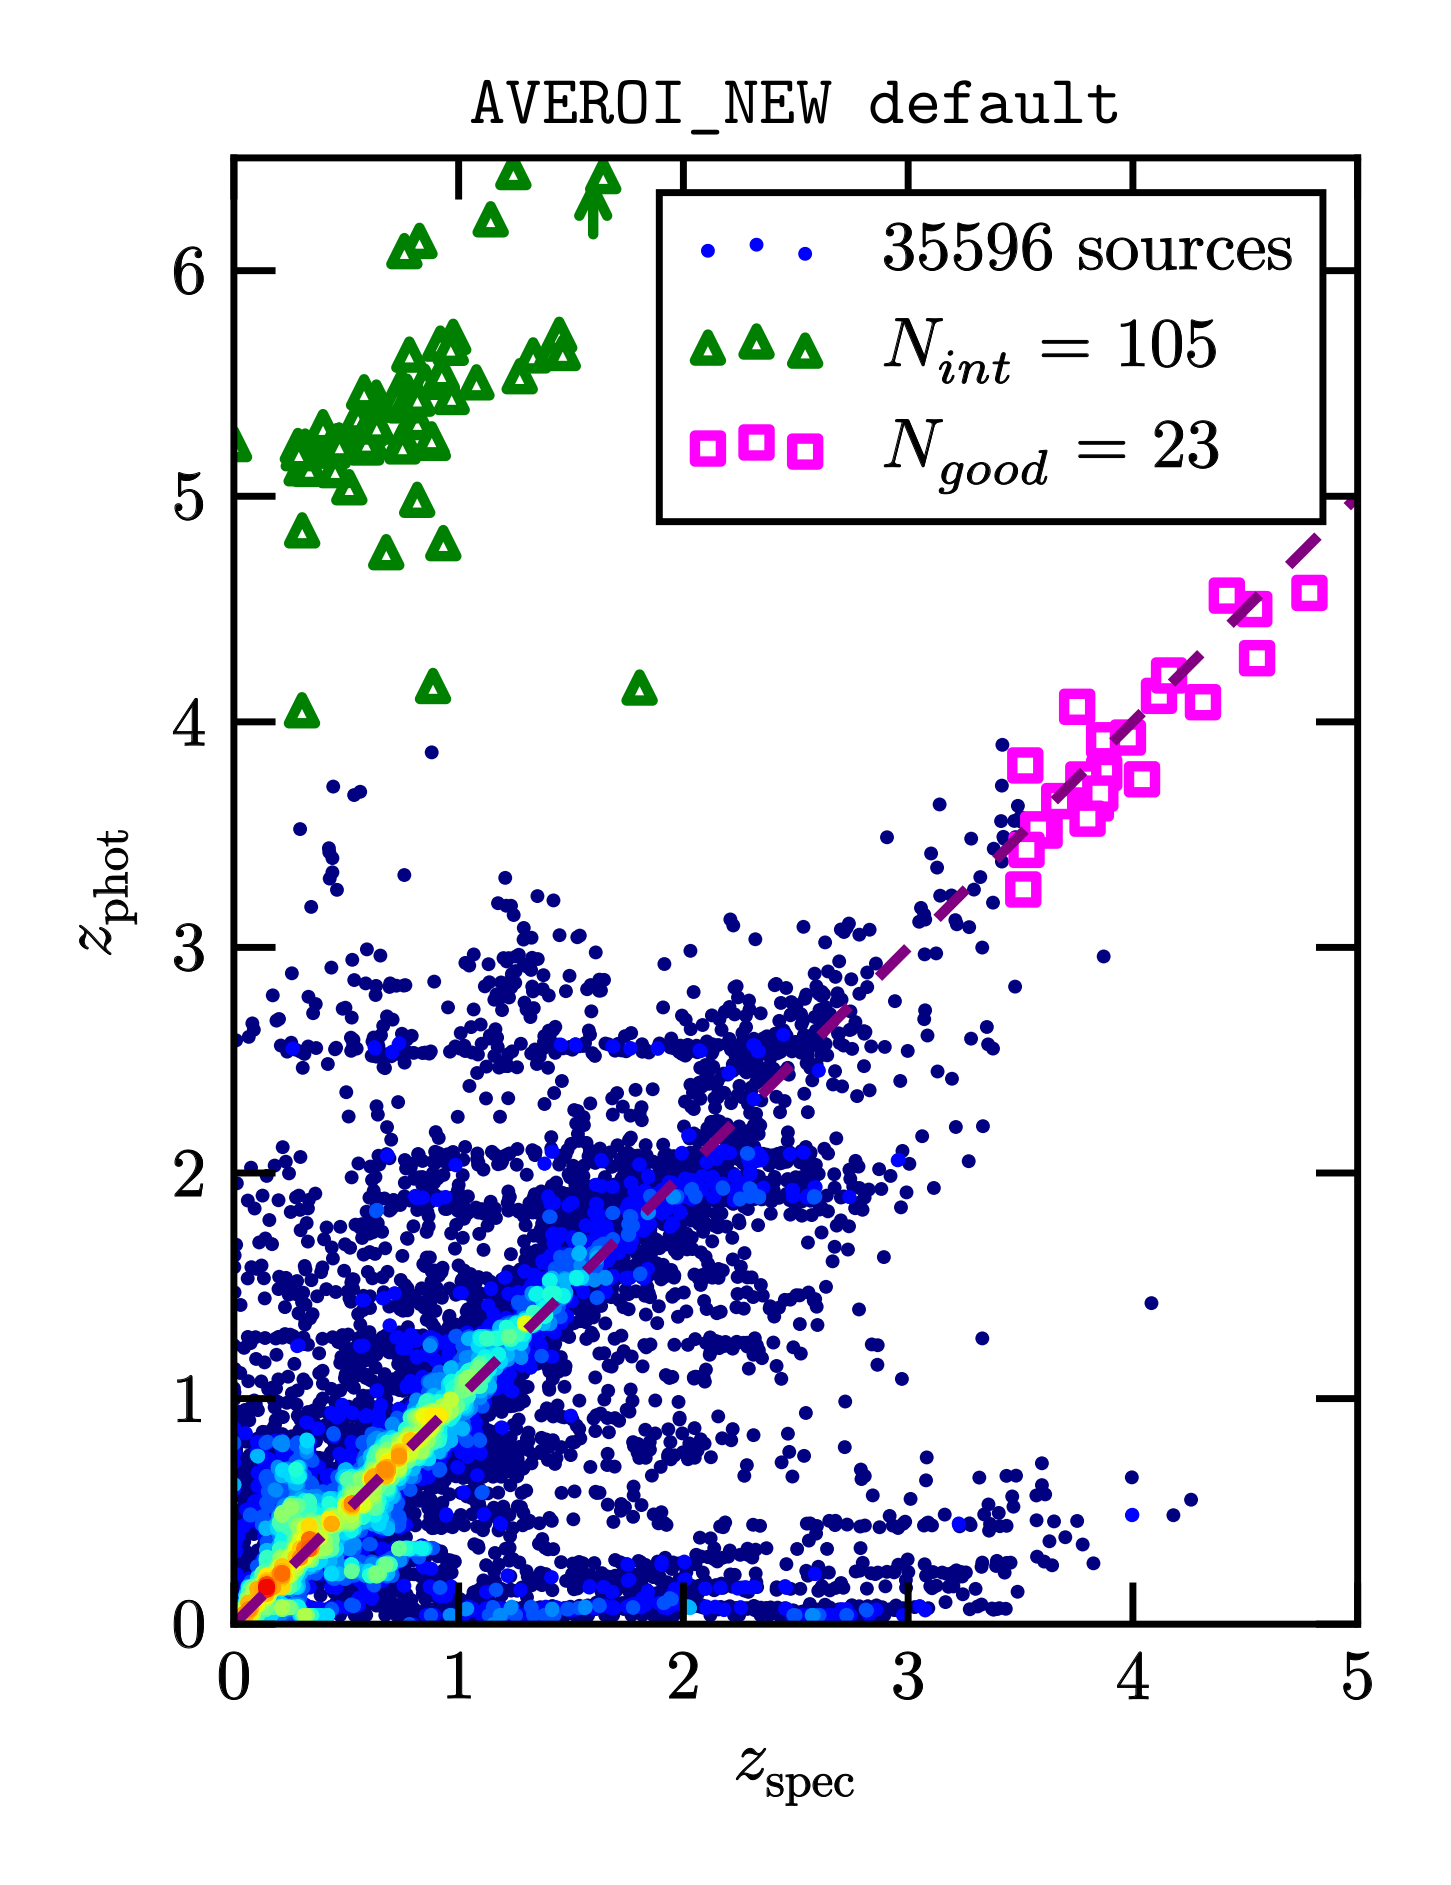
\includegraphics[clip, width=0.5\textwidth]{Chapter3/Figs/template_basic.png}}
\subfloat[\label{fig:cosmos_basic}]{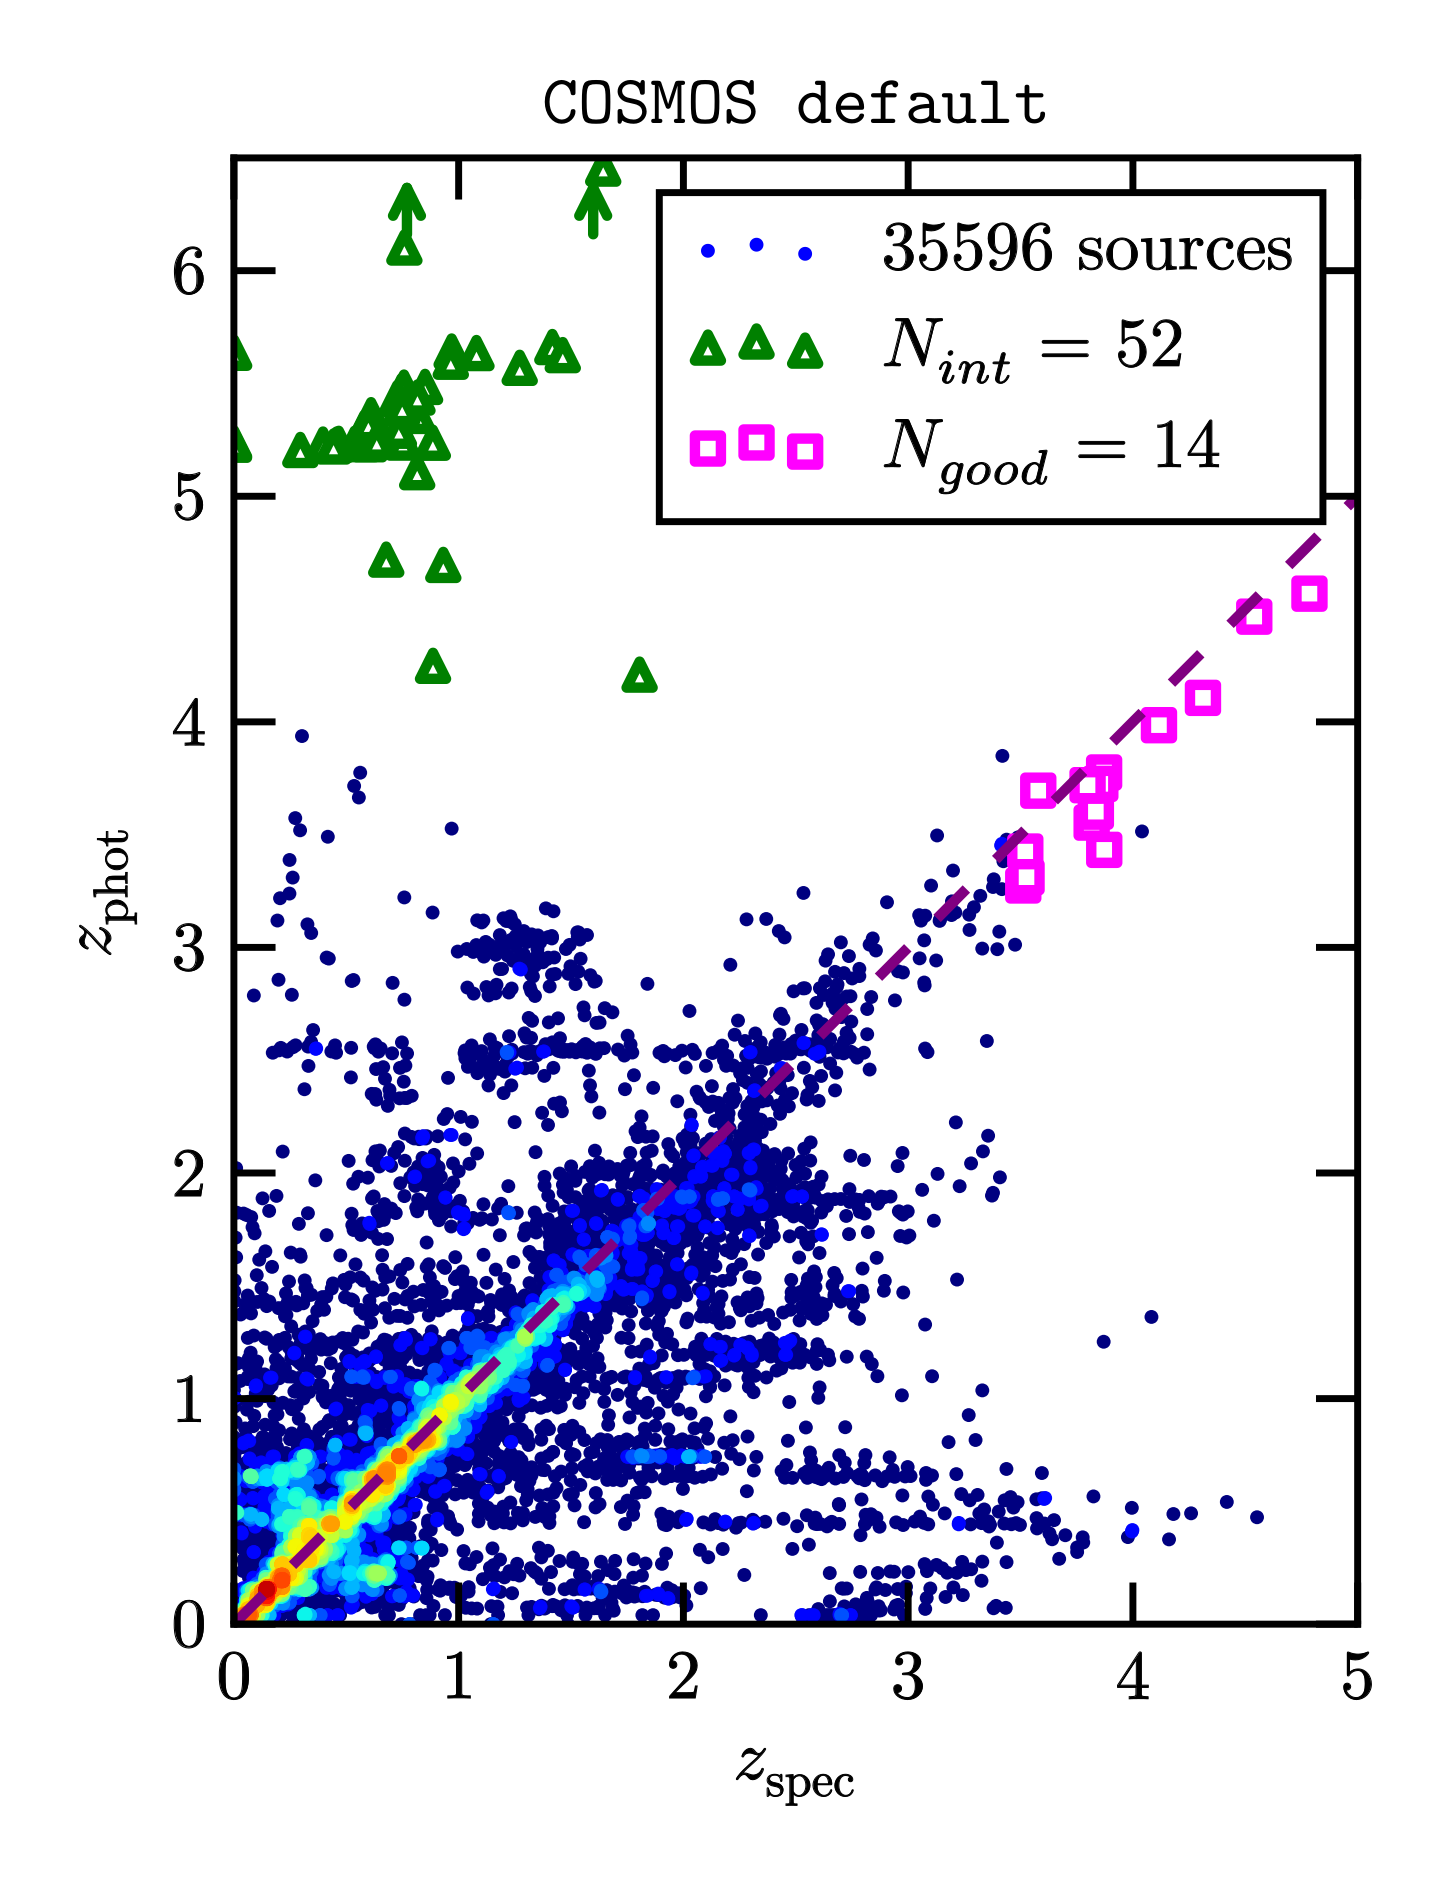
\includegraphics[clip, width=0.5\textwidth]{Chapter3/Figs/template_cosmos.png}}
\caption[\texorpdfstring{$z_{\mathrm{spec}}$}{} vs \texorpdfstring{$z_{\mathrm{phot}}$}{} distributions of the test configurations]{The distribution of spectroscopic vs photometric redshifts for all configurations listed in Table \ref{table:photoz_test}. The colour of each data point shows the number density in bins of 0.01, on a rainbow scale of blue (low) to red (high). The colours have been normalised over all figures, so that the same colour depicts the same number density across all plots. The pink squares represent good high-redshift fits, defined via $N_{\mathrm{good}}$ in Equation \ref{eqn:N_good}. The green triangles show low-redshift interlopers defined via $N_{\mathrm{int}}$ in Equation \ref{eqn:N_int}. The green arrows in some figures indicate interlopers for which the photometric redshift falls outside the plotted window (i.e. $z_{\mathrm{phot}}>6.5$).}\label{fig:photoz_distribution}
\end{figure}

\begin{figure}
\ContinuedFloat
\subfloat[\label{fig:less_ext}]{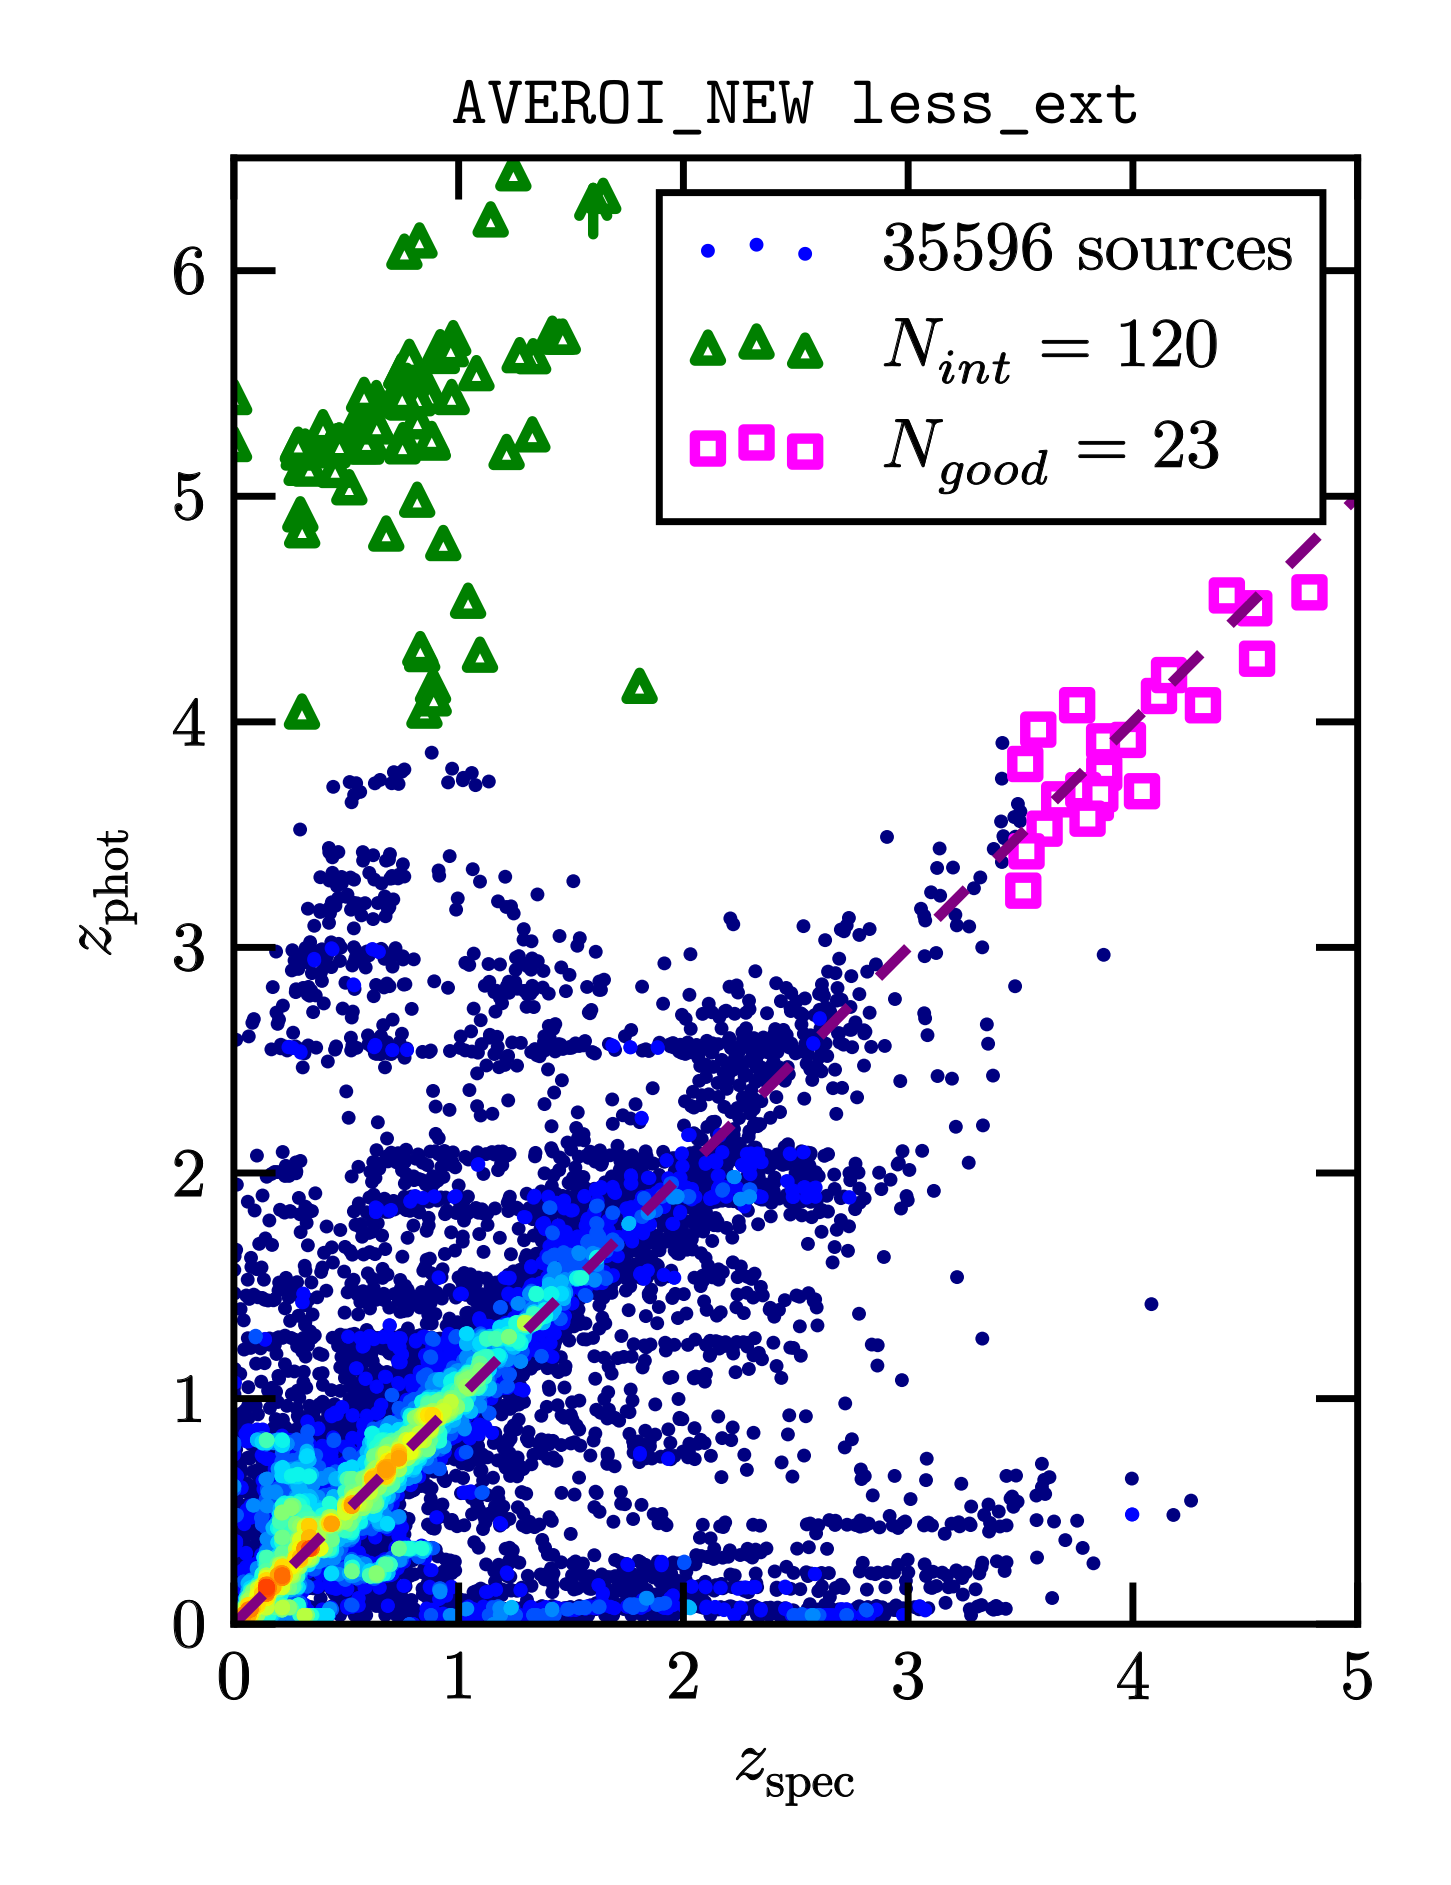
\includegraphics[clip, width=0.5\textwidth]{Chapter3/Figs/template_less_ext.png}}
\subfloat[\label{fig:more_ext}]{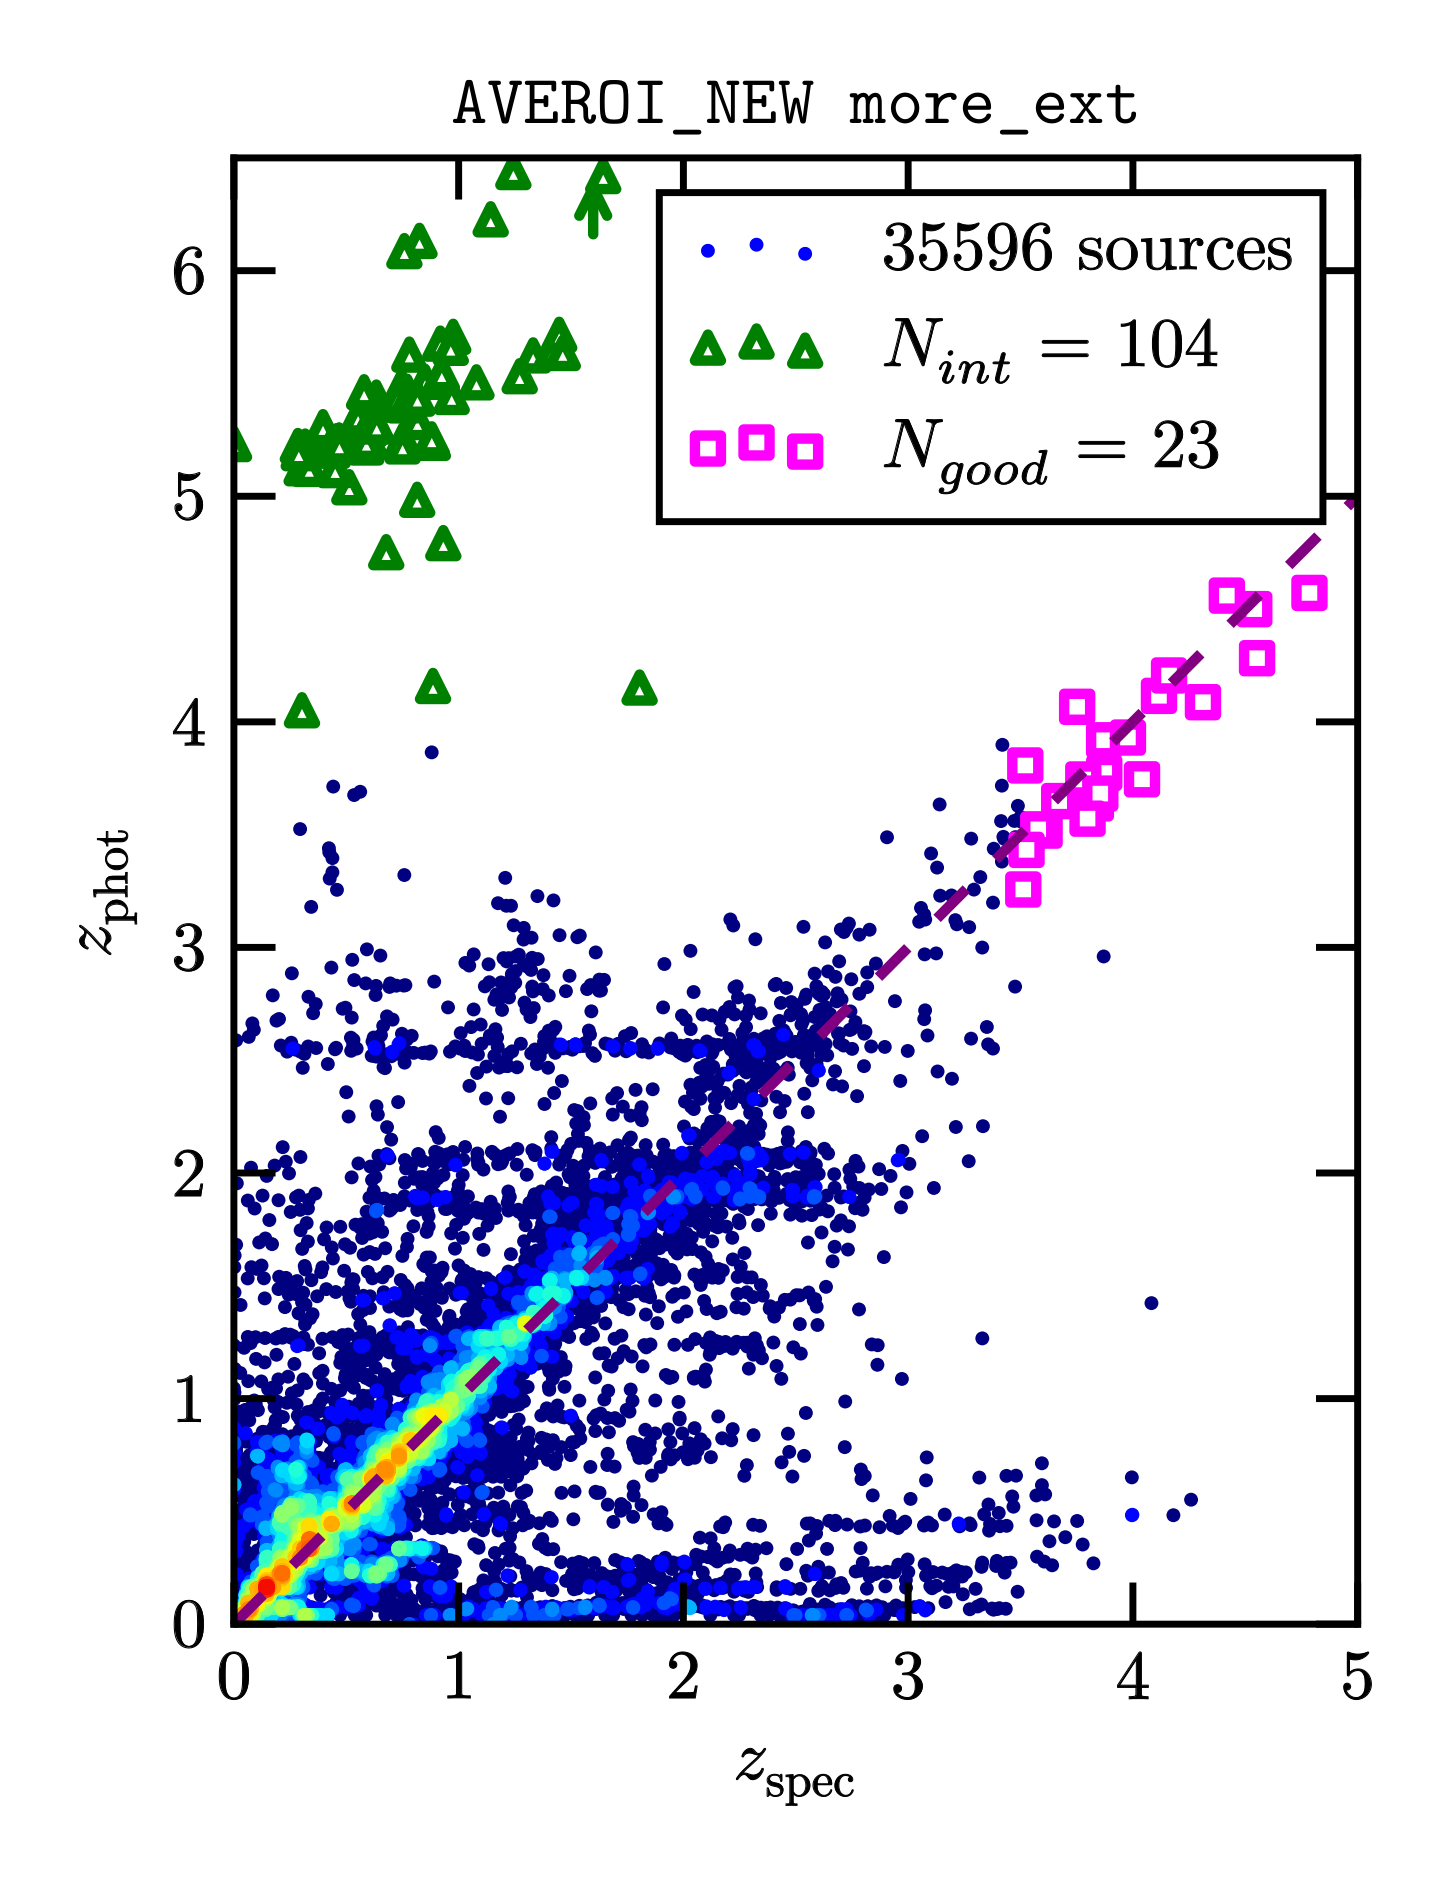
\includegraphics[clip, width=0.5\textwidth]{Chapter3/Figs/template_more_ext.png}}

\subfloat[]{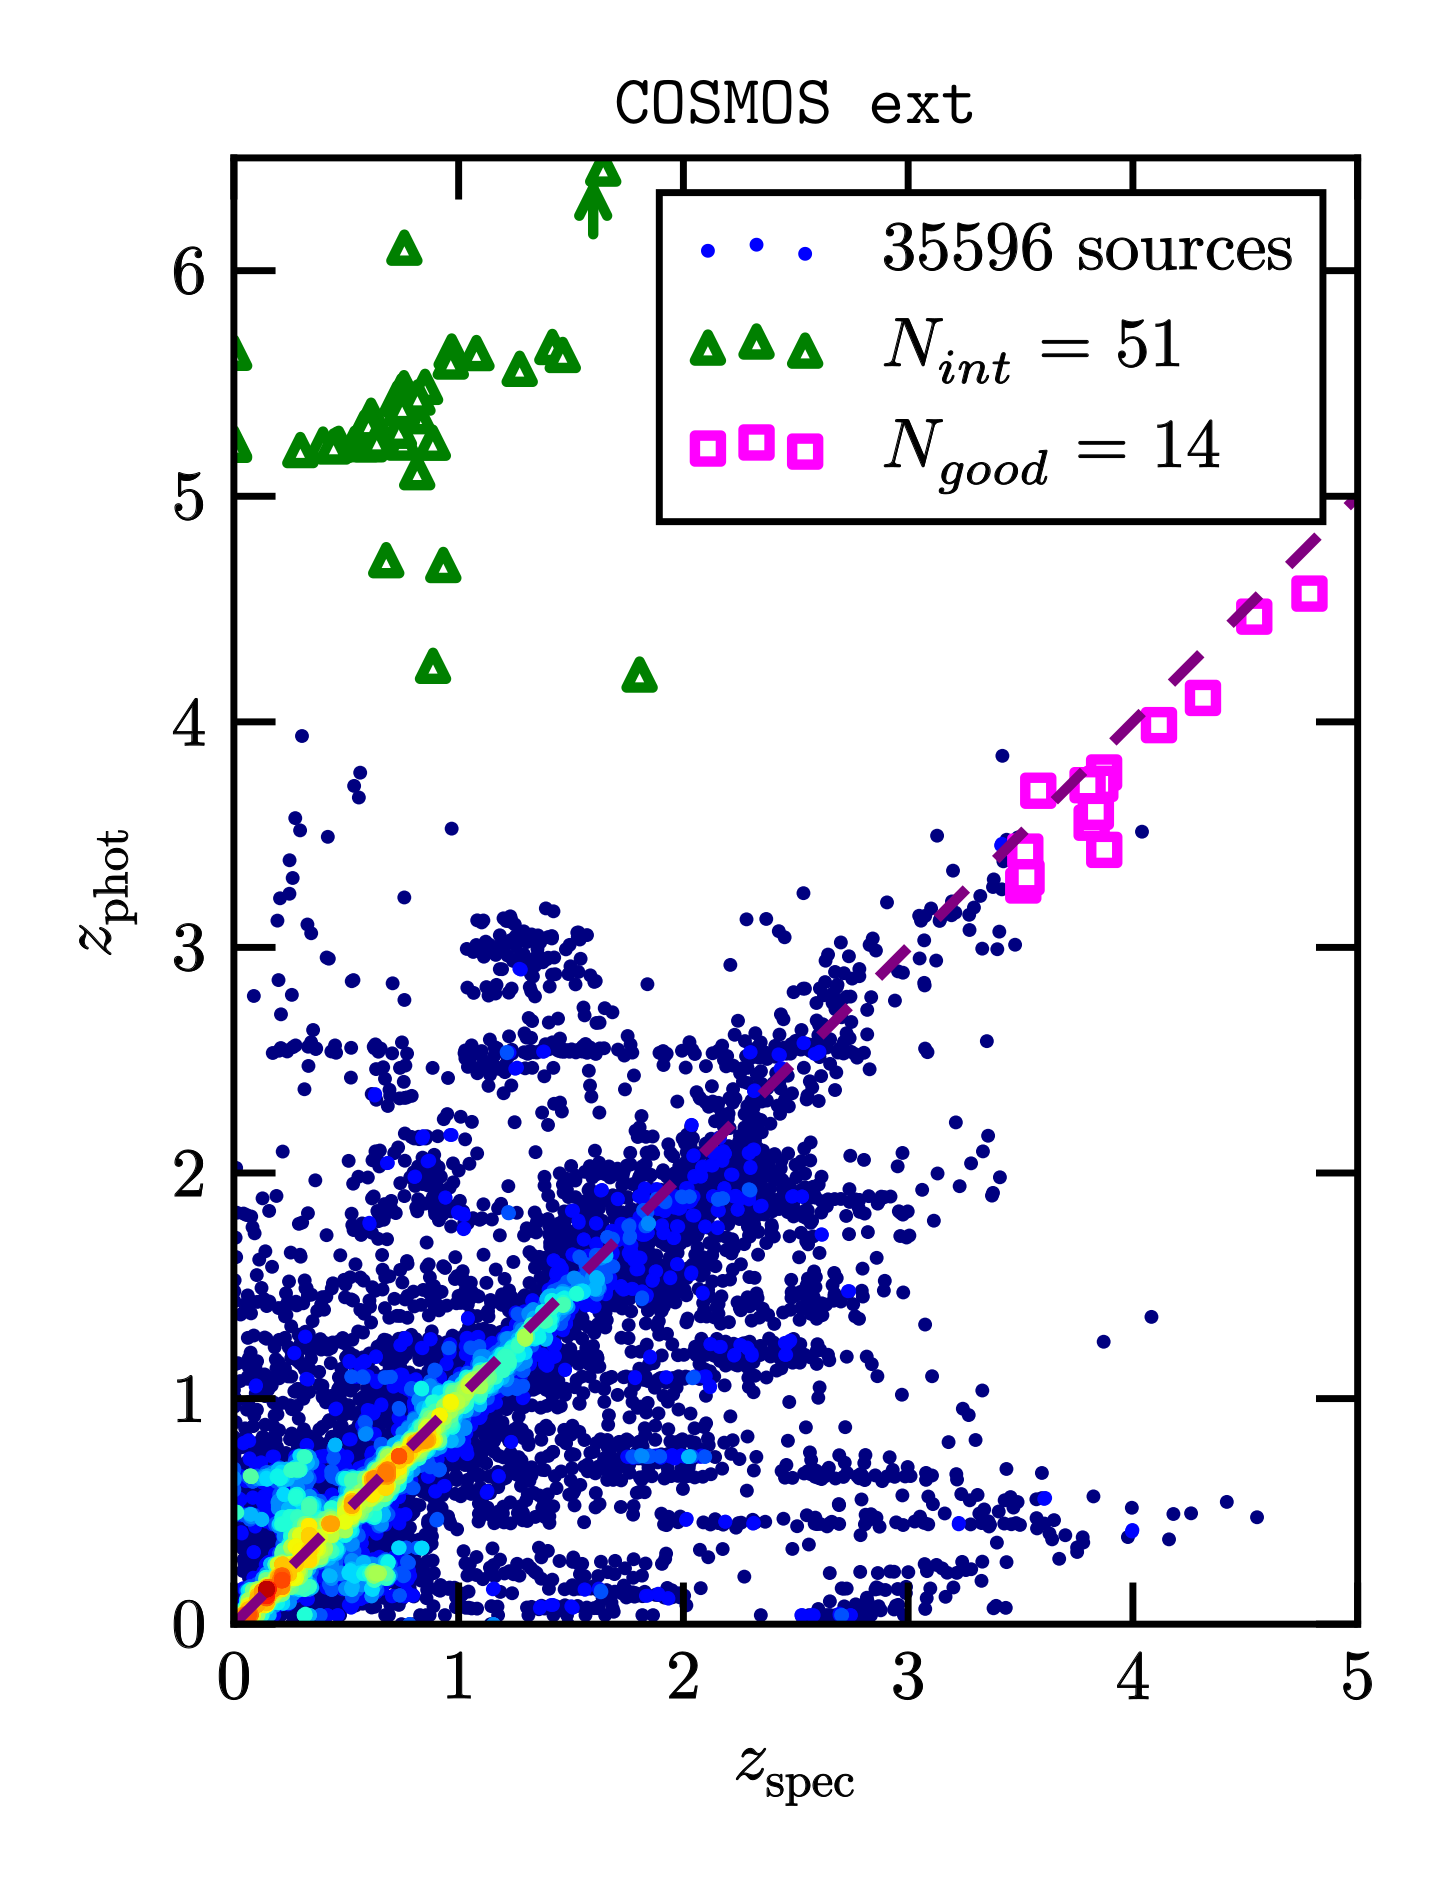
\includegraphics[clip, width=0.5\textwidth]{Chapter3/Figs/template_cosmos_ext.png}}
\subfloat[]{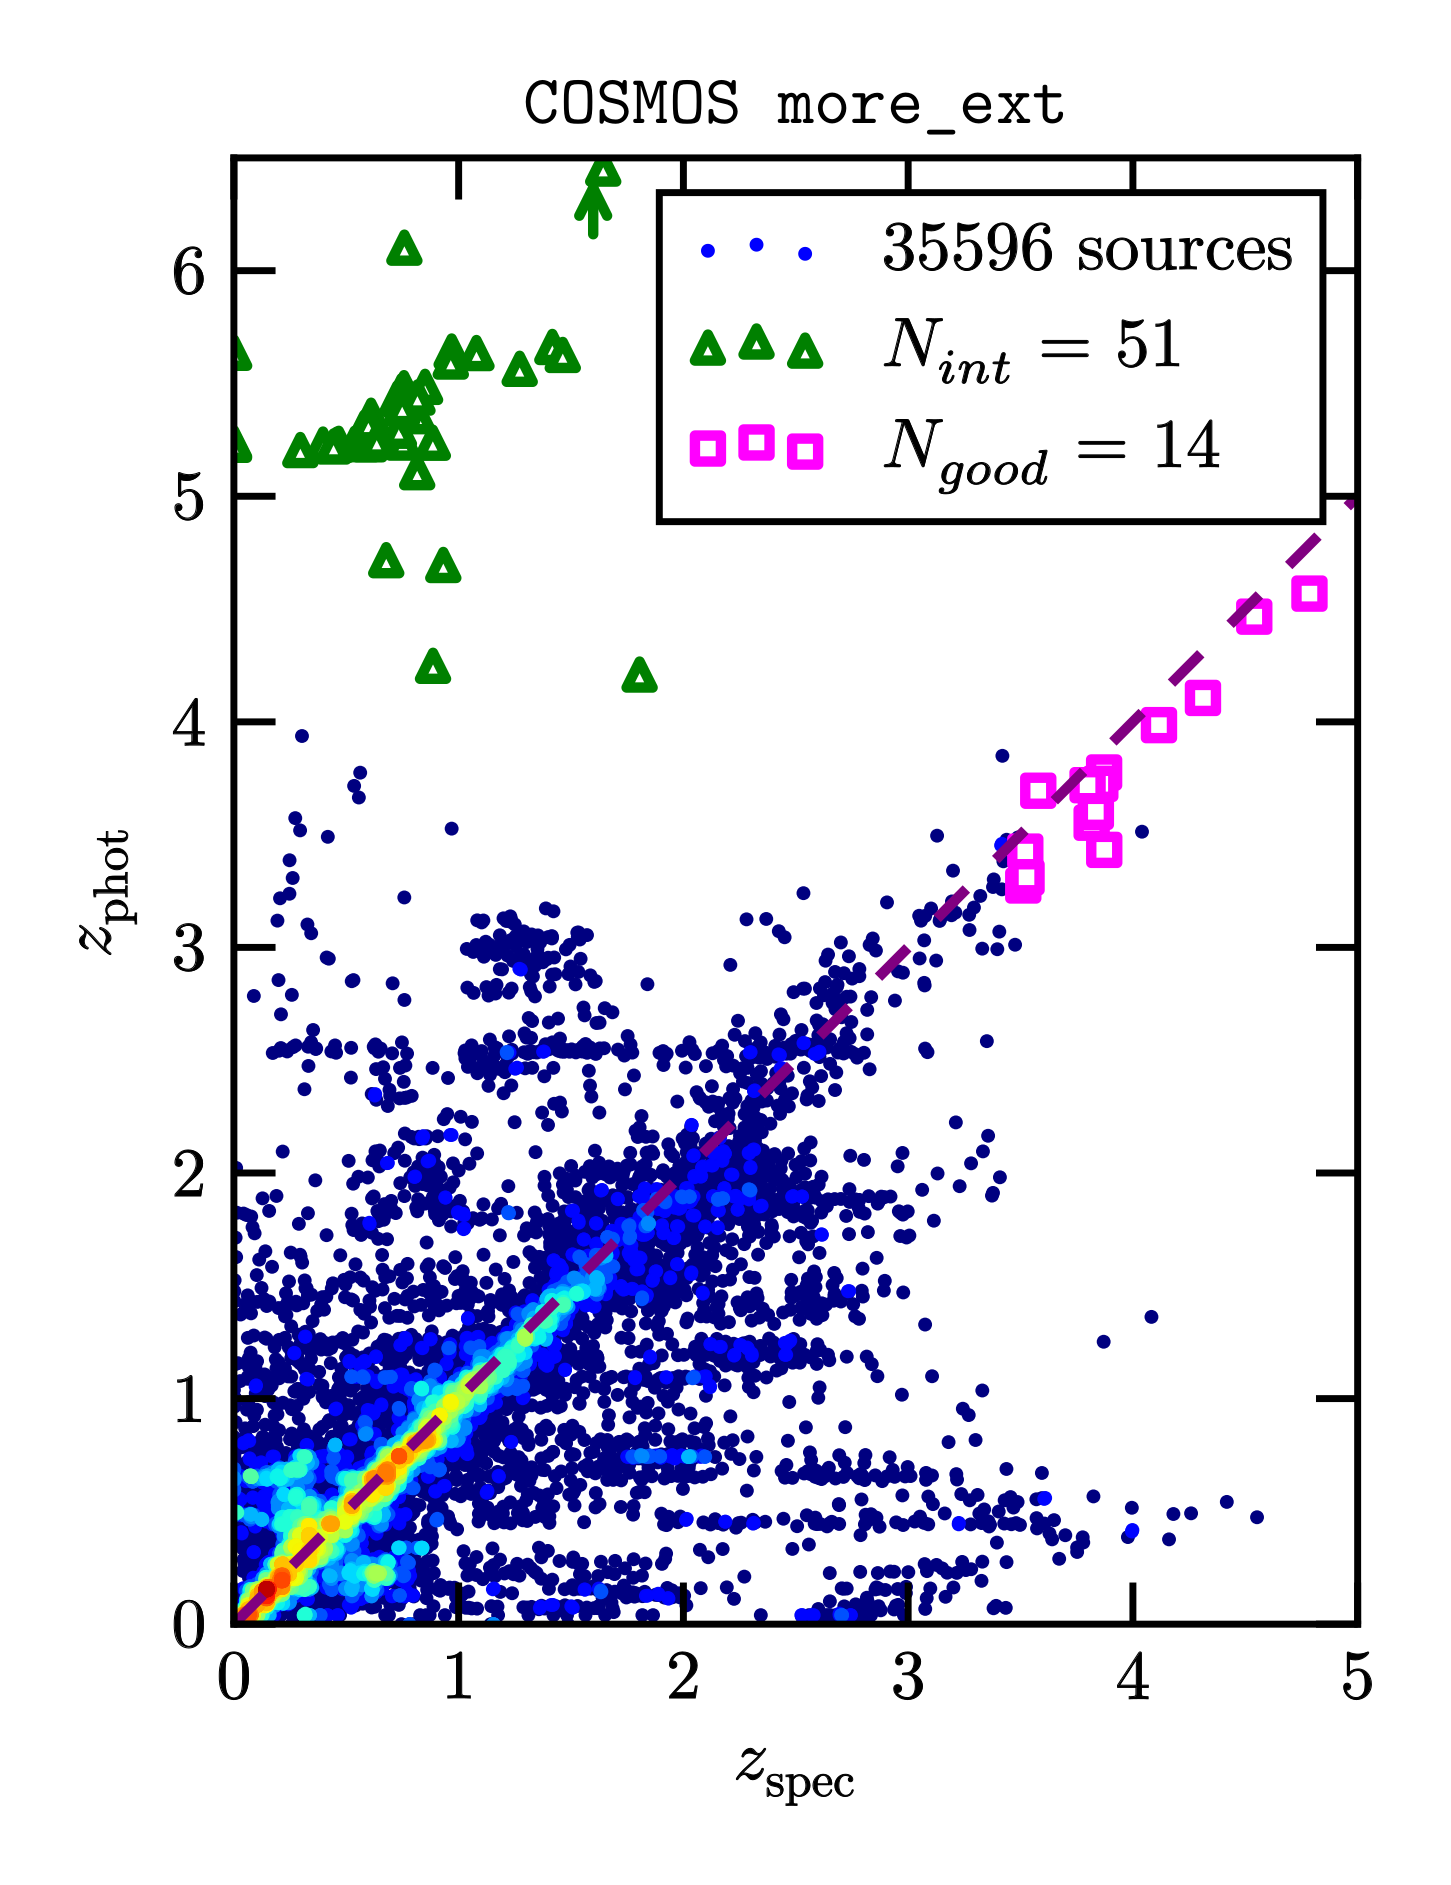
\includegraphics[clip, width=0.5\textwidth]{Chapter3/Figs/template_cosmos_more_ext.png}}
\caption{\textit{continued}}
\end{figure}

\begin{figure}
\ContinuedFloat
\subfloat[\label{fig:no_emlines}]{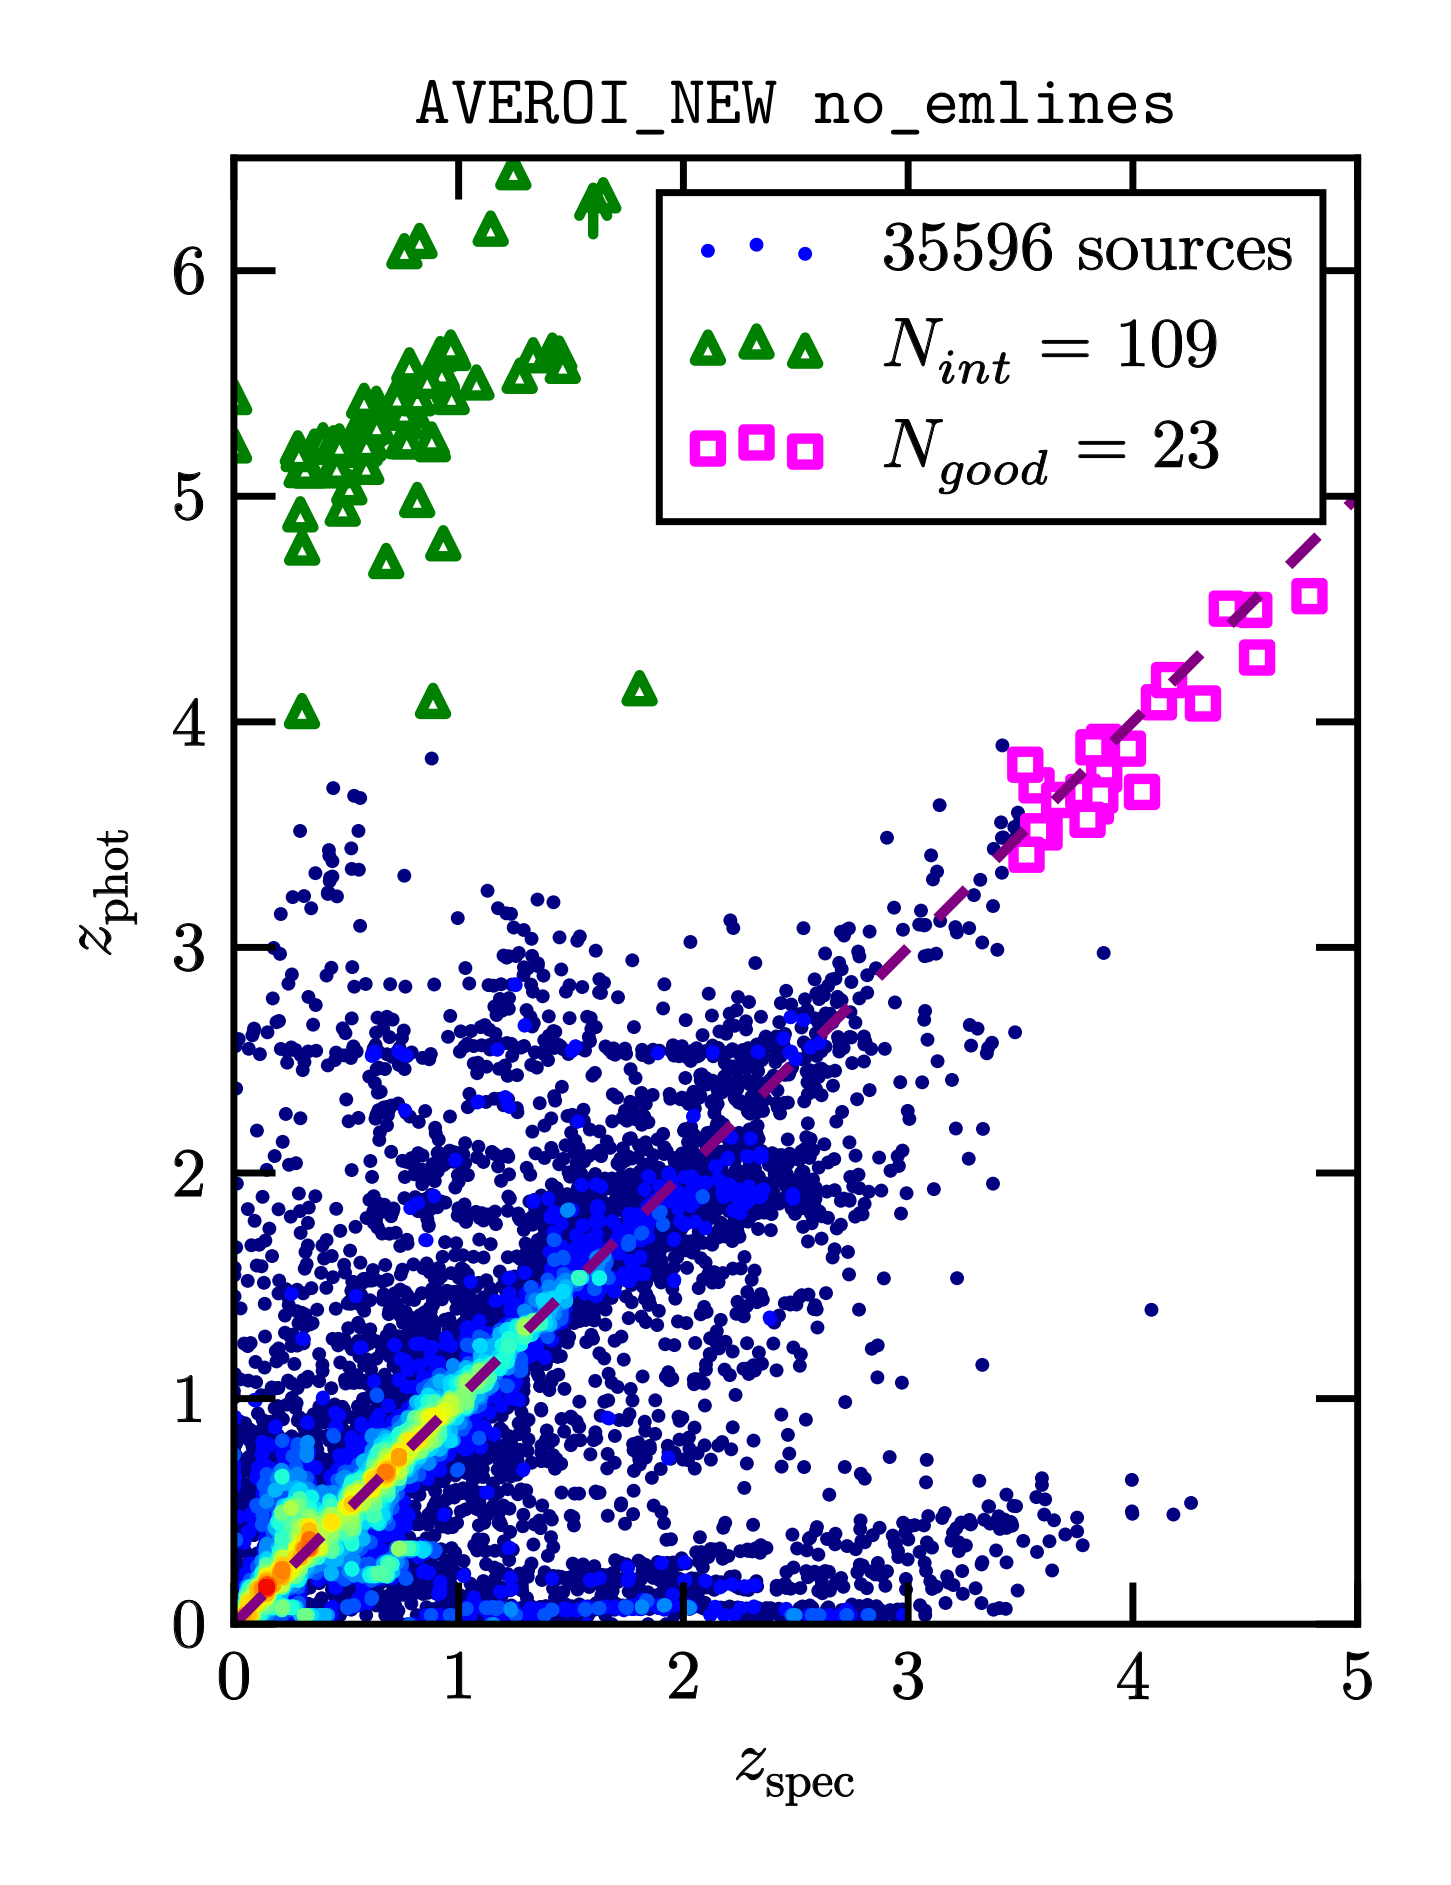
\includegraphics[clip, width=0.5\textwidth]{Chapter3/Figs/template_no_emlines.png}}
\subfloat[\label{fig:cosmos_no_emlines}]{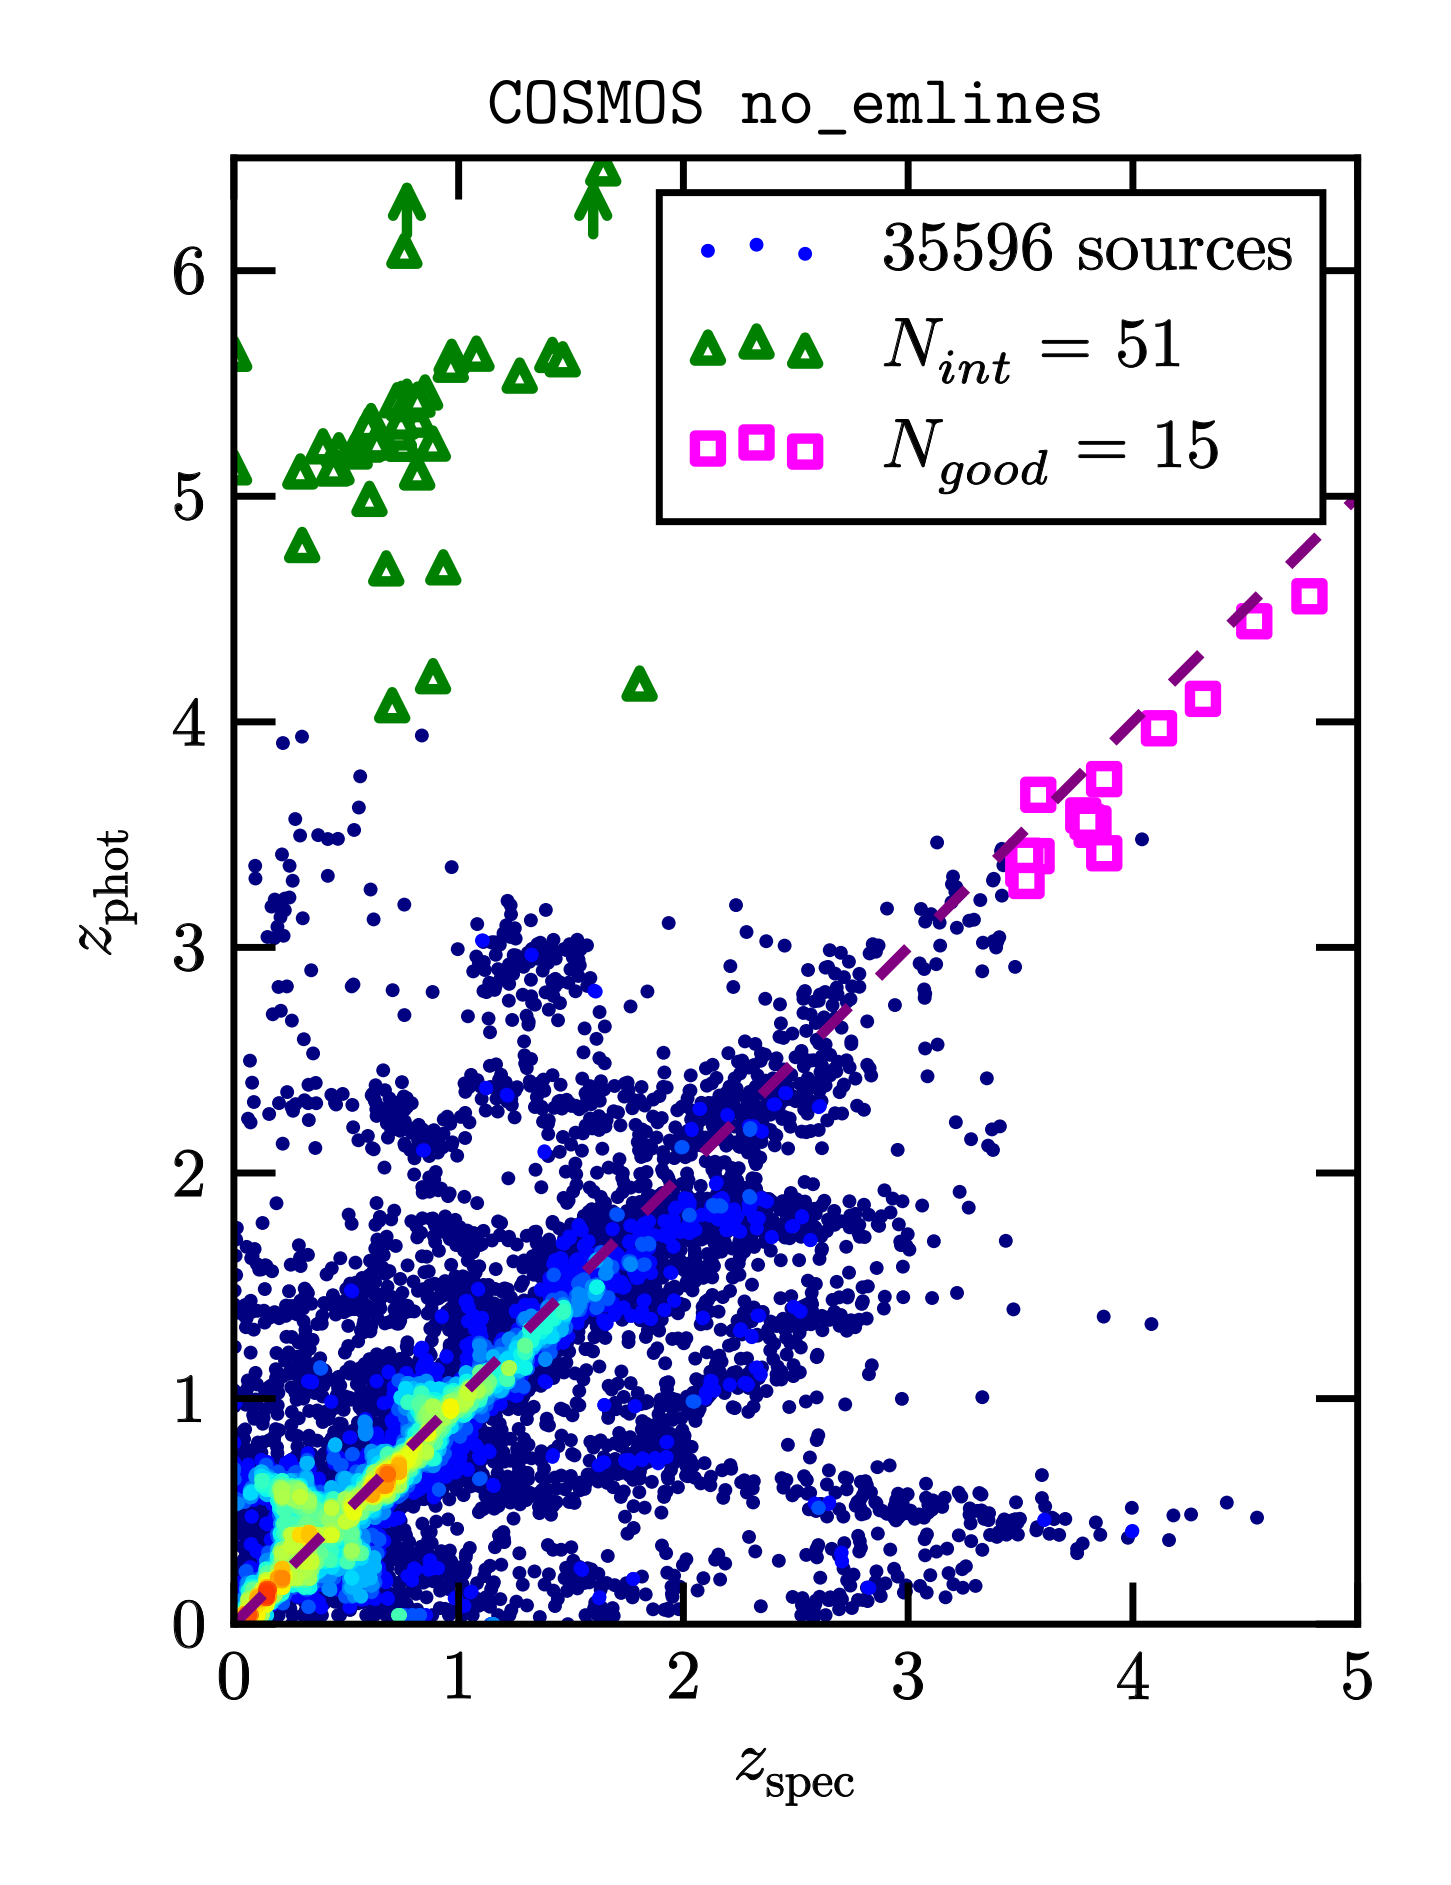
\includegraphics[clip, width=0.5\textwidth]{Chapter3/Figs/template_cosmos_no_emlines.png}}

\subfloat[\label{fig:no_prior}]{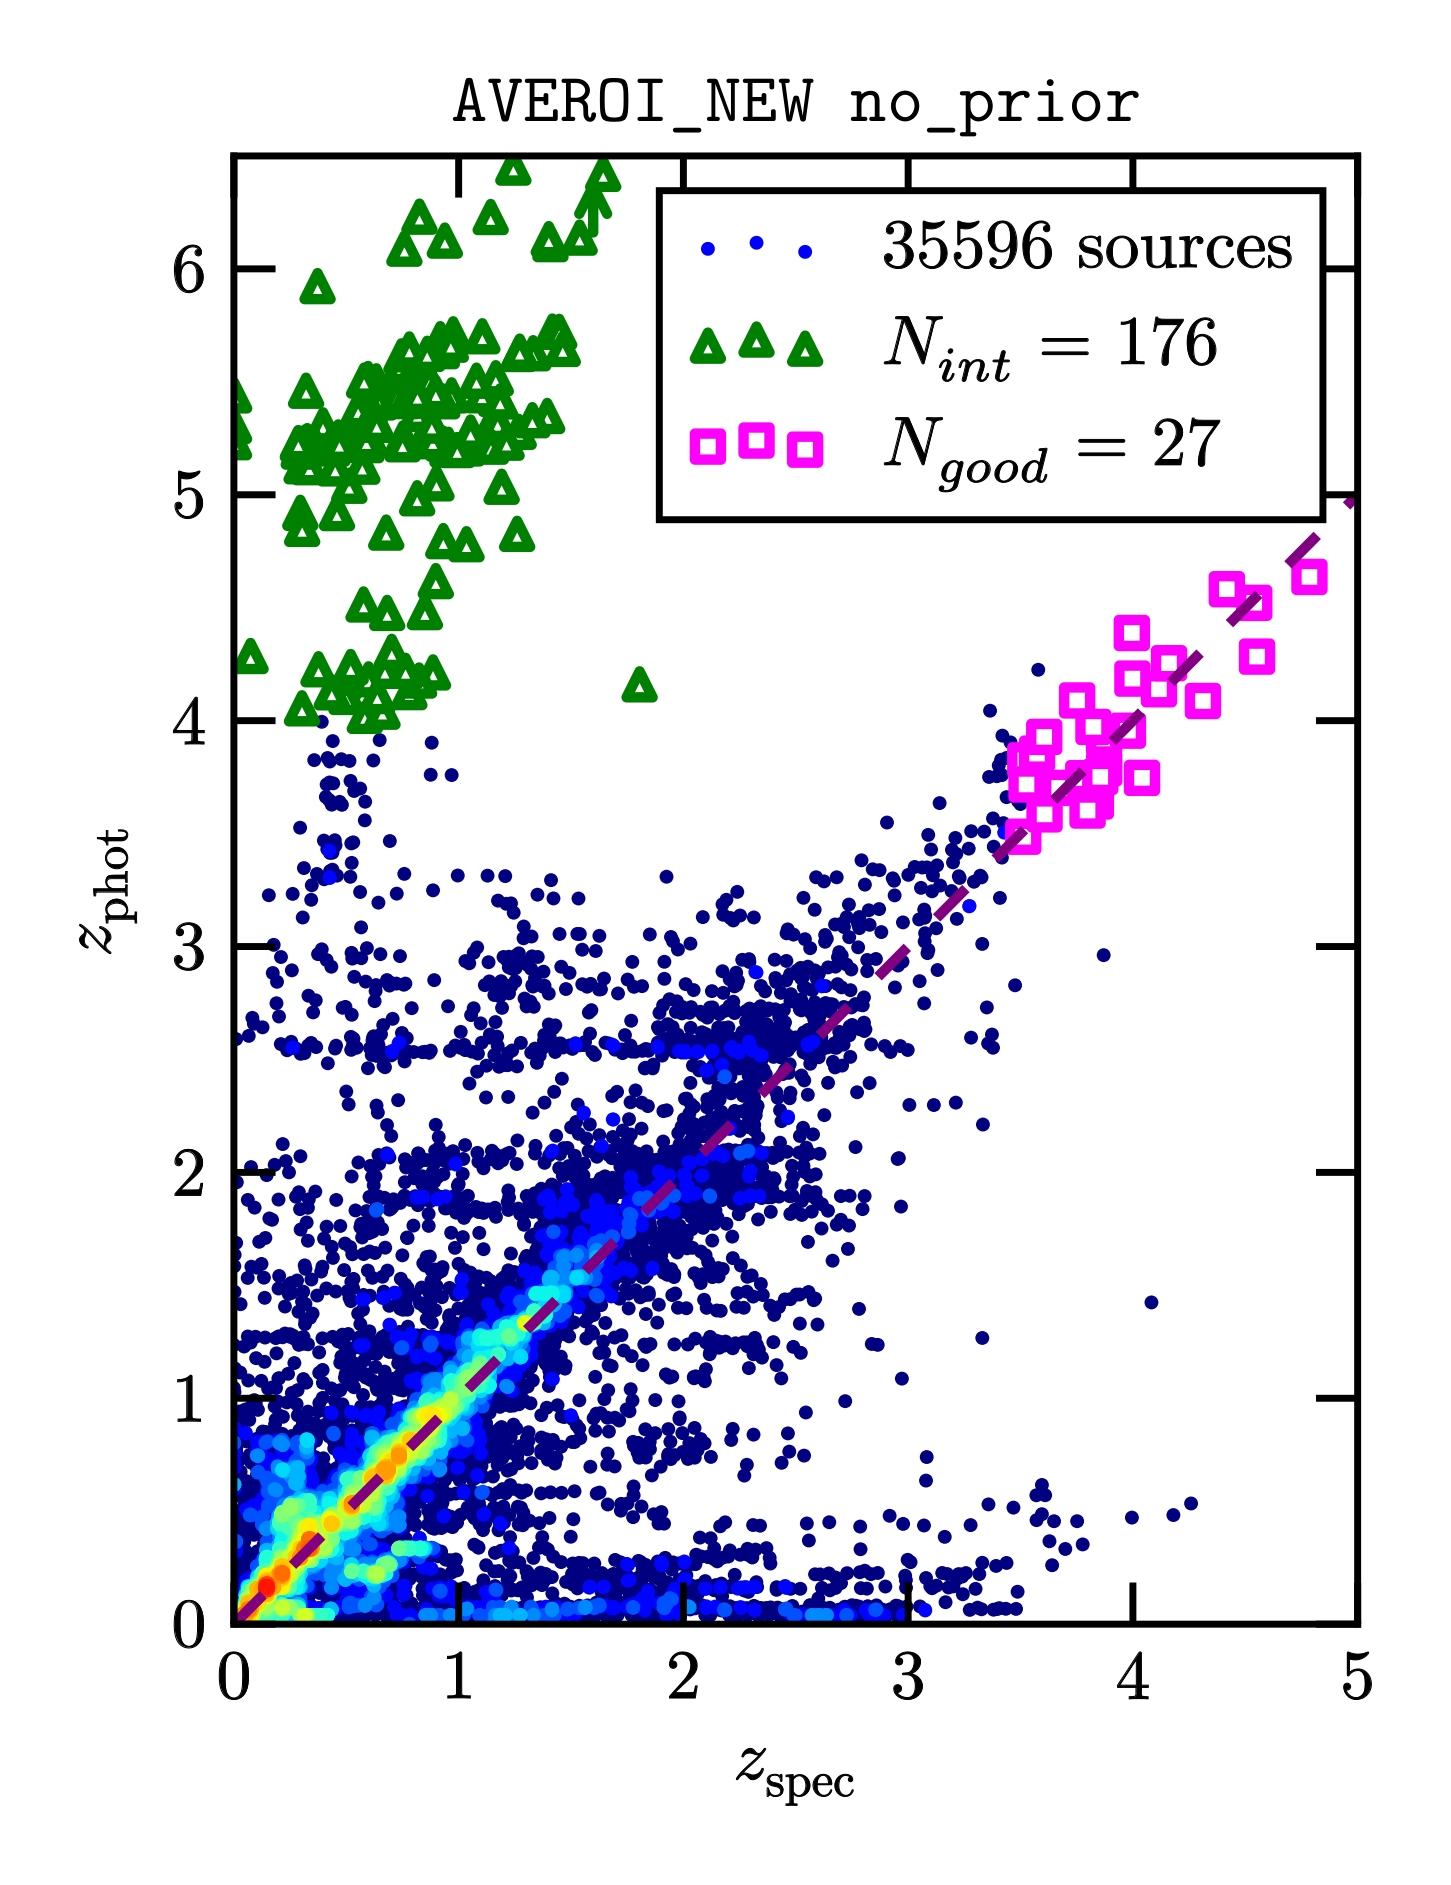
\includegraphics[clip, width=0.5\textwidth]{Chapter3/Figs/template_no_prior.png}}
\subfloat[\label{fig:cosmos_no_prior}]{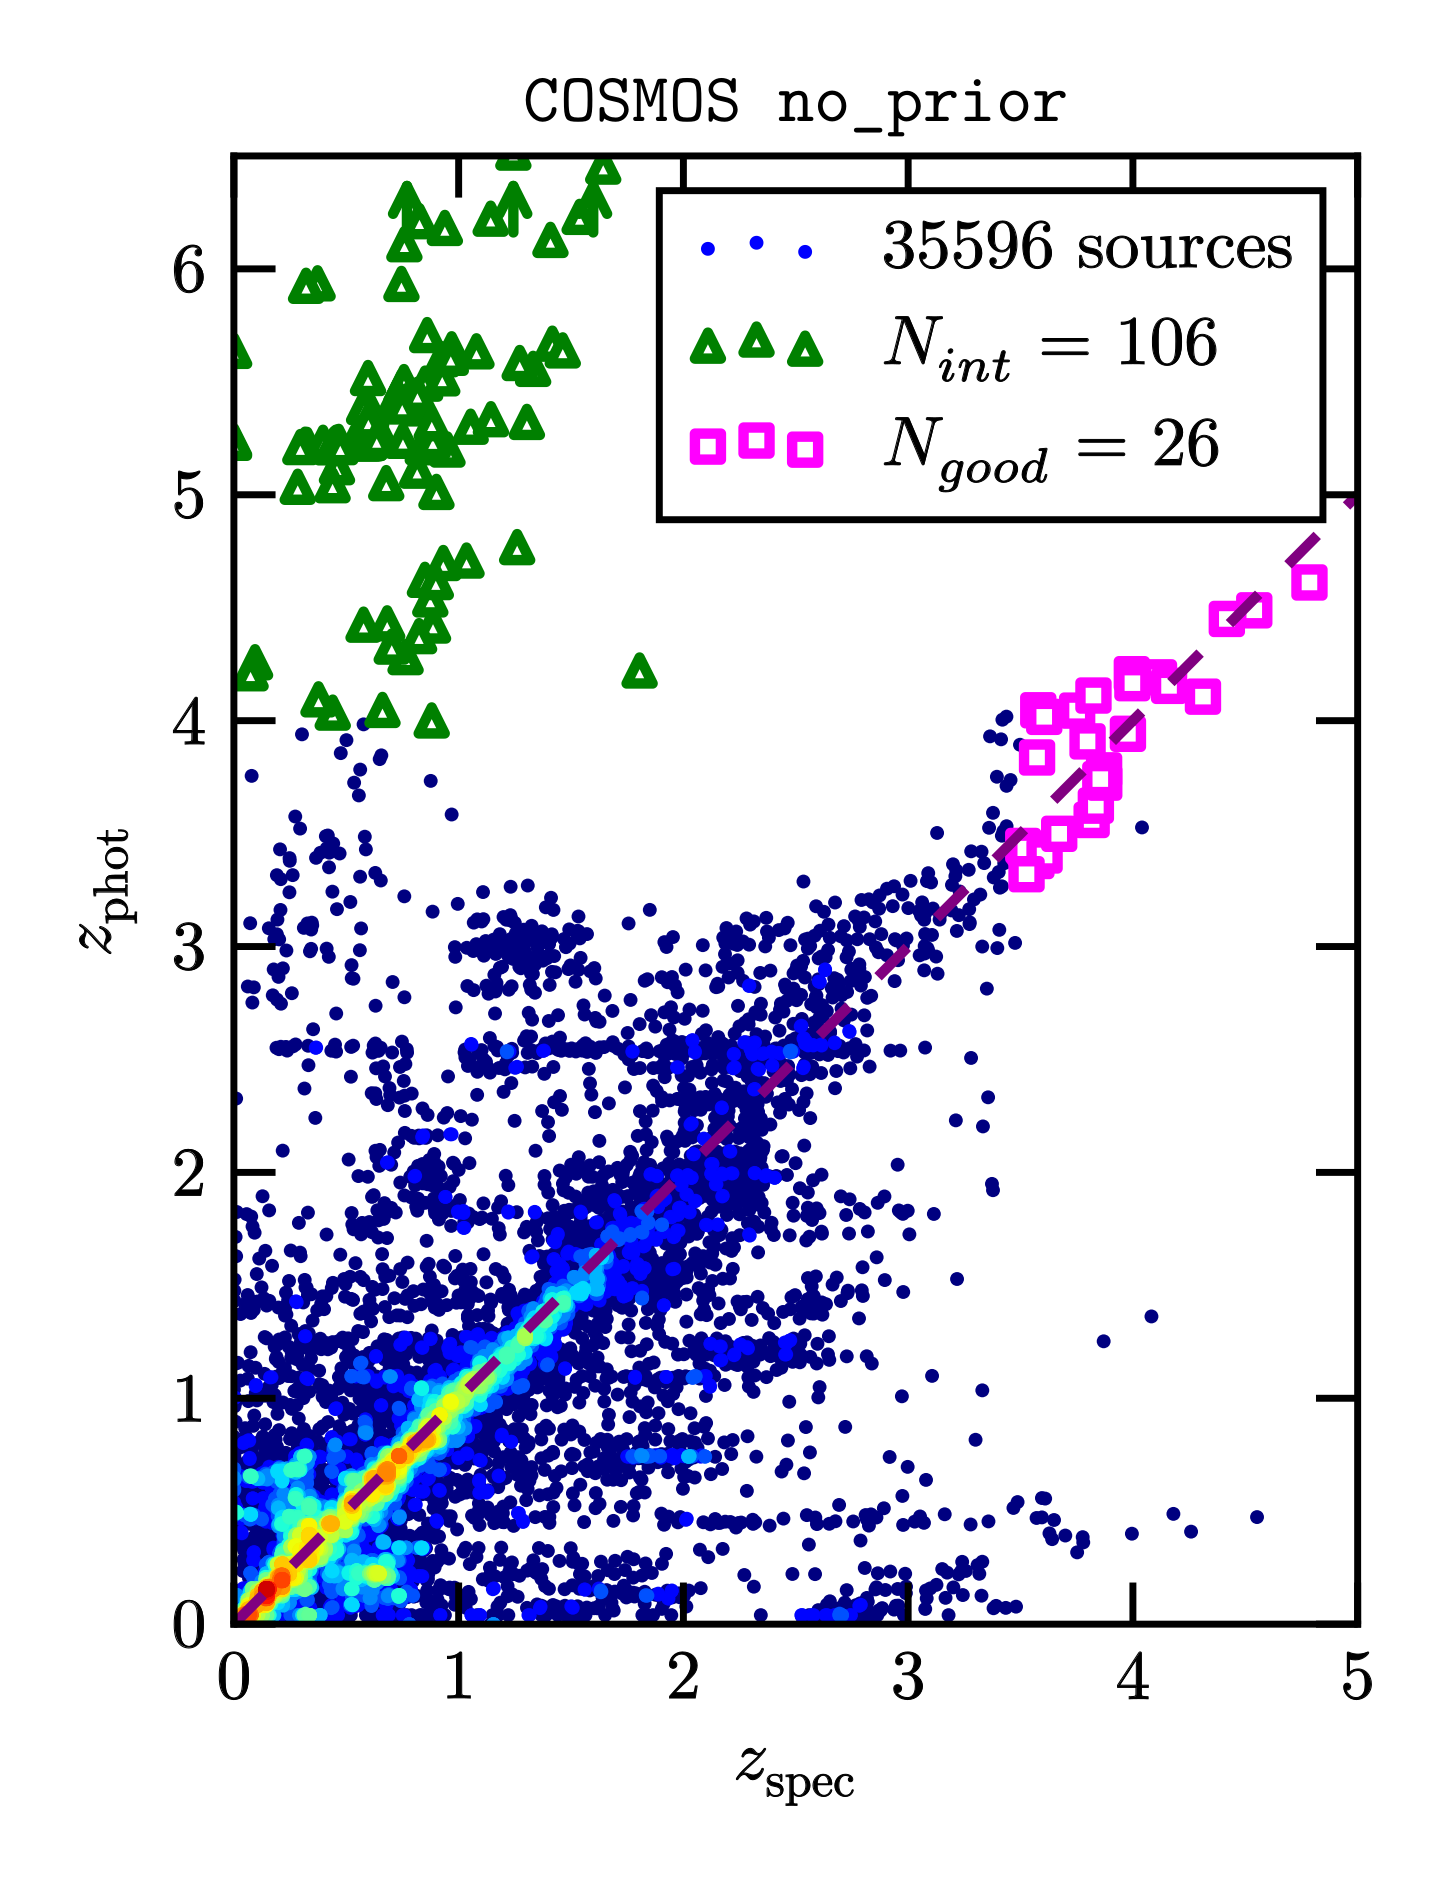
\includegraphics[clip, width=0.5\textwidth]{Chapter3/Figs/template_cosmos_no_prior.png}}
\caption{\textit{continued}}
\end{figure}

\begin{figure}
\ContinuedFloat
\subfloat[]{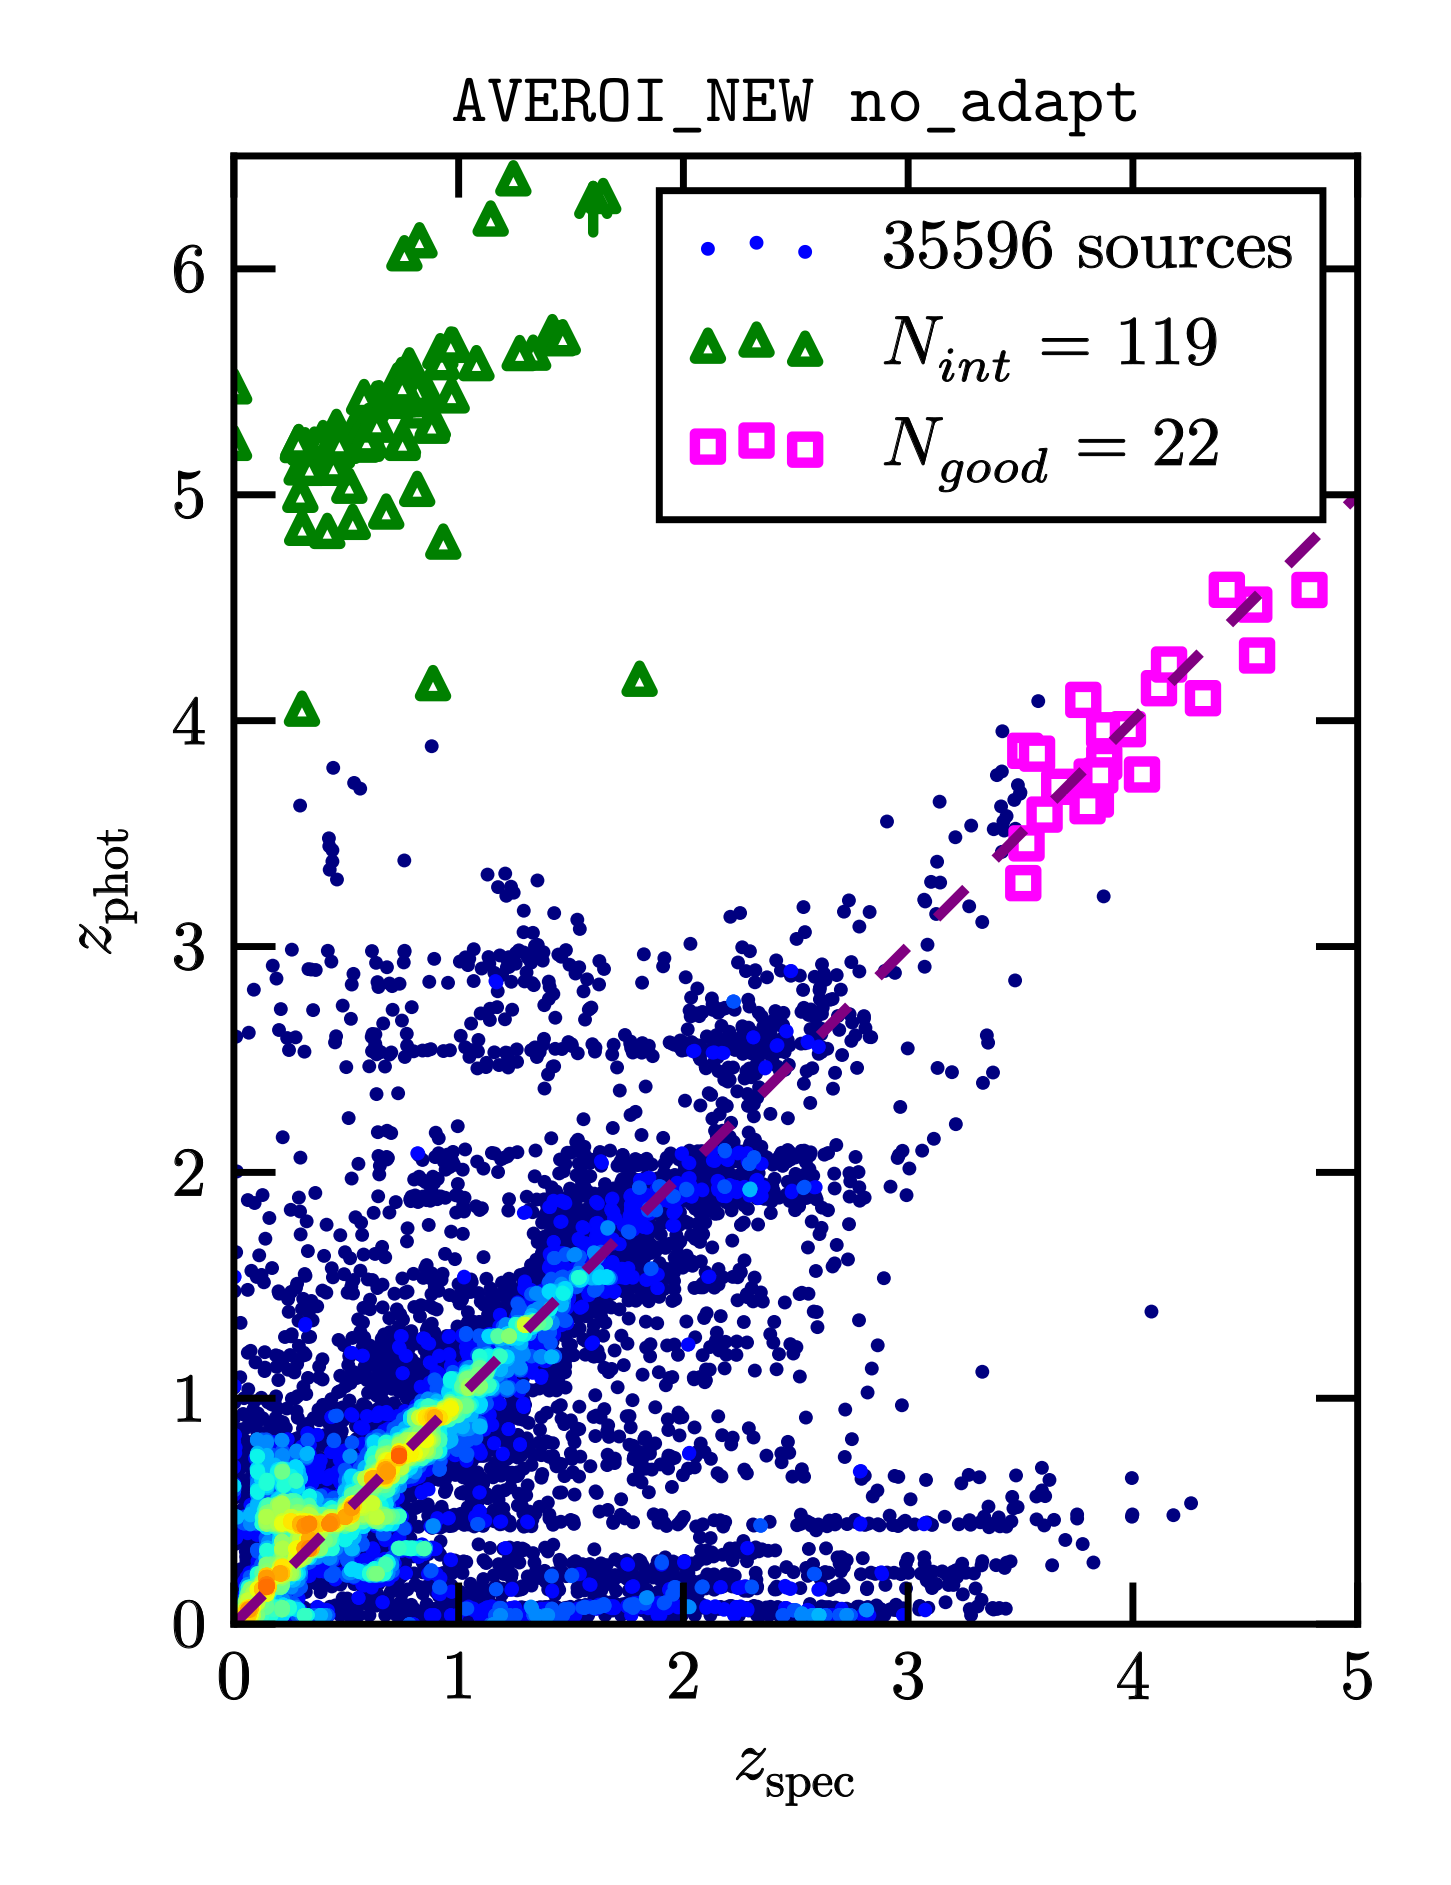
\includegraphics[clip, width=0.5\textwidth]{Chapter3/Figs/template_no_adapt.png}}
\subfloat[\label{fig:cosmos_no_adapt}]{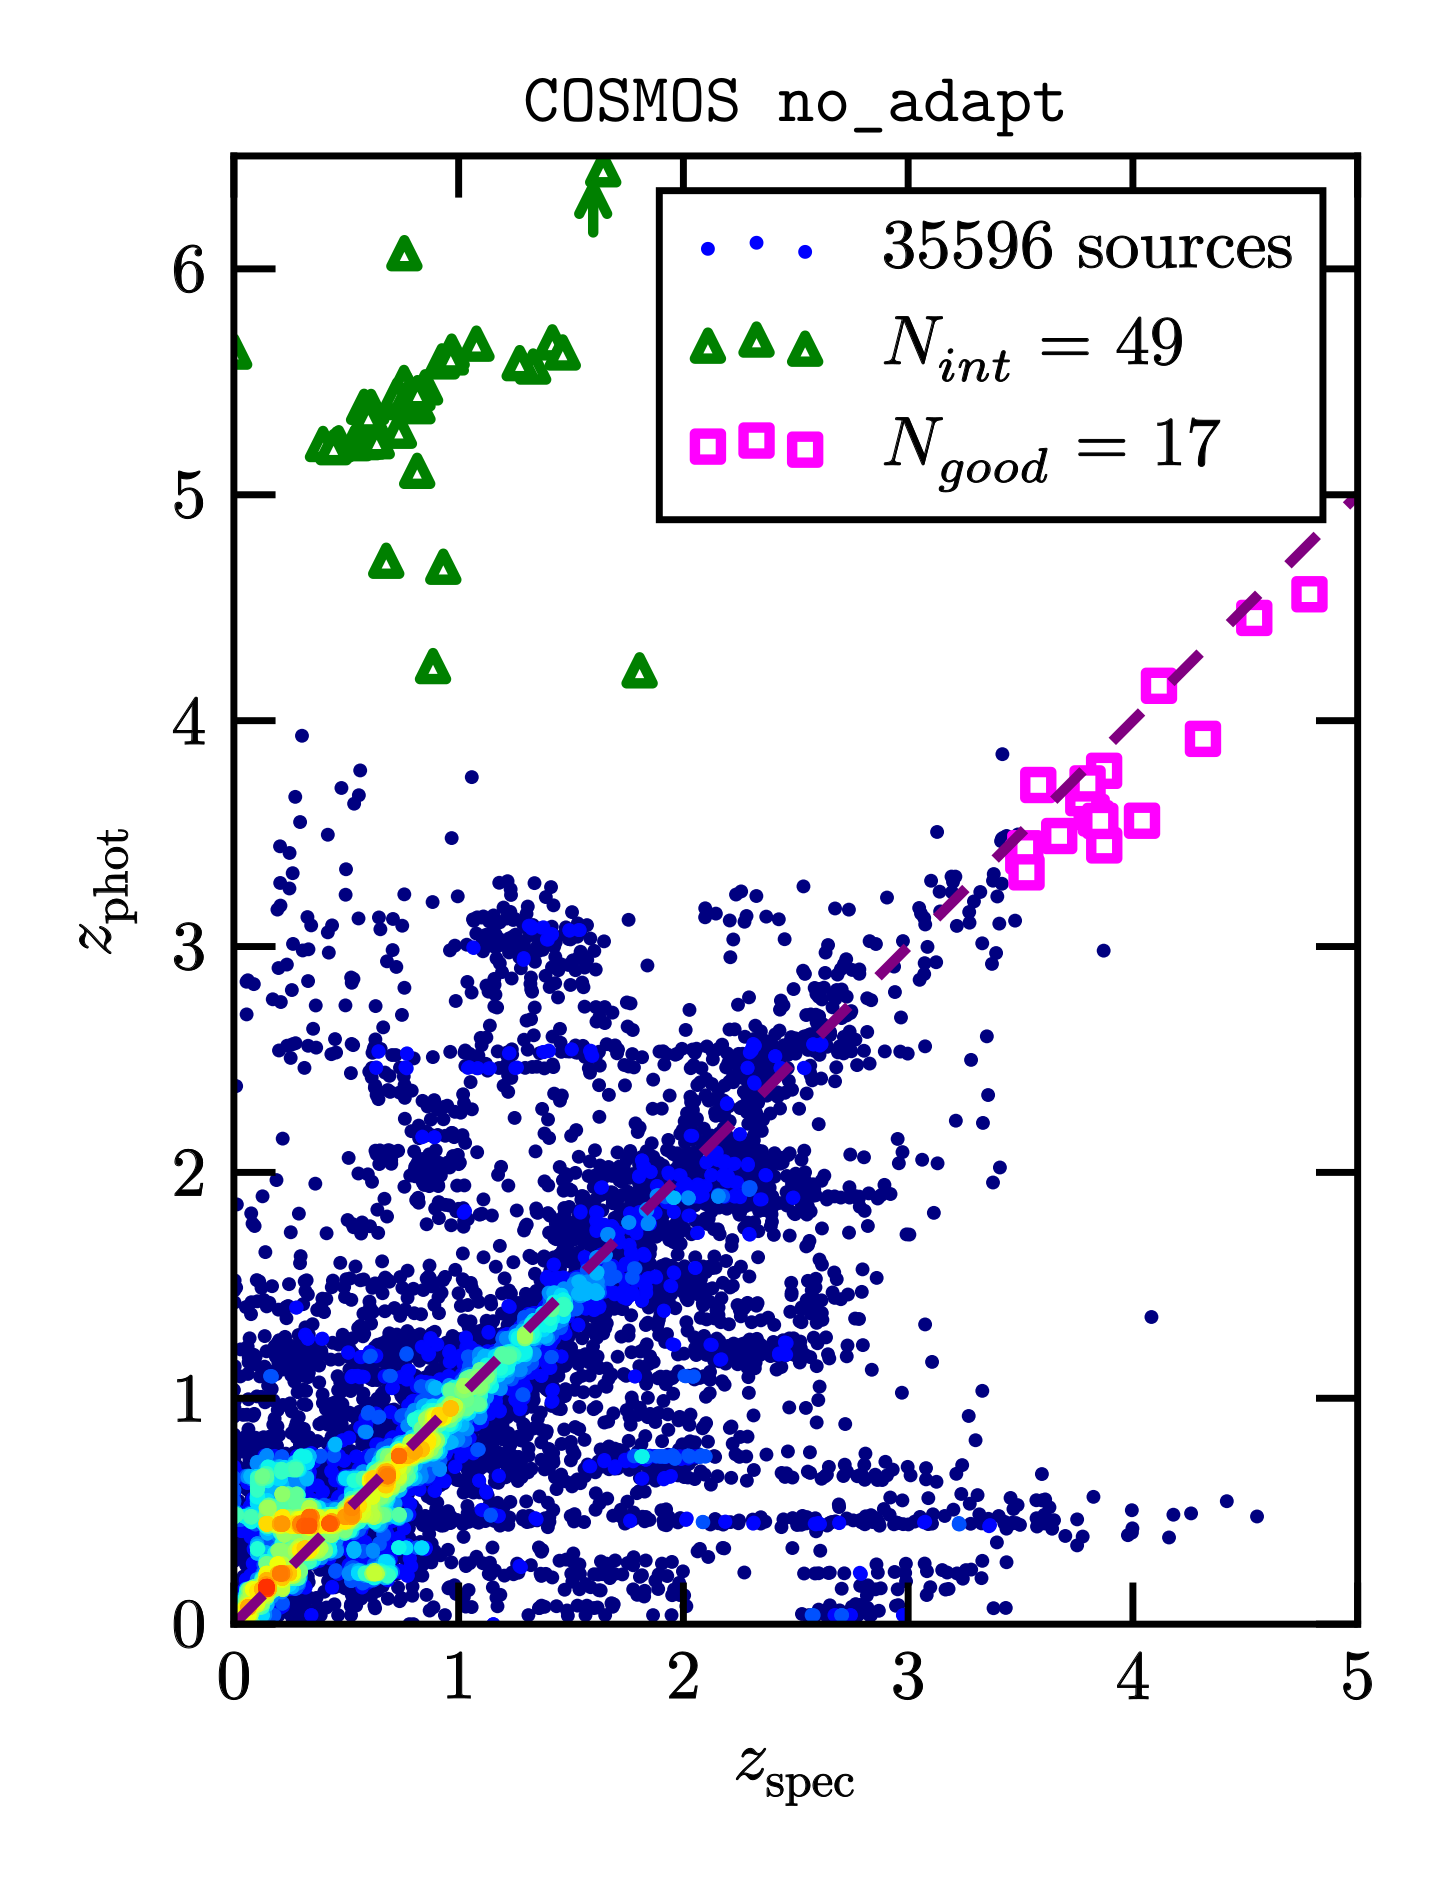
\includegraphics[clip, width=0.5\textwidth]{Chapter3/Figs/template_cosmos_no_adapt.png}}

\subfloat[]{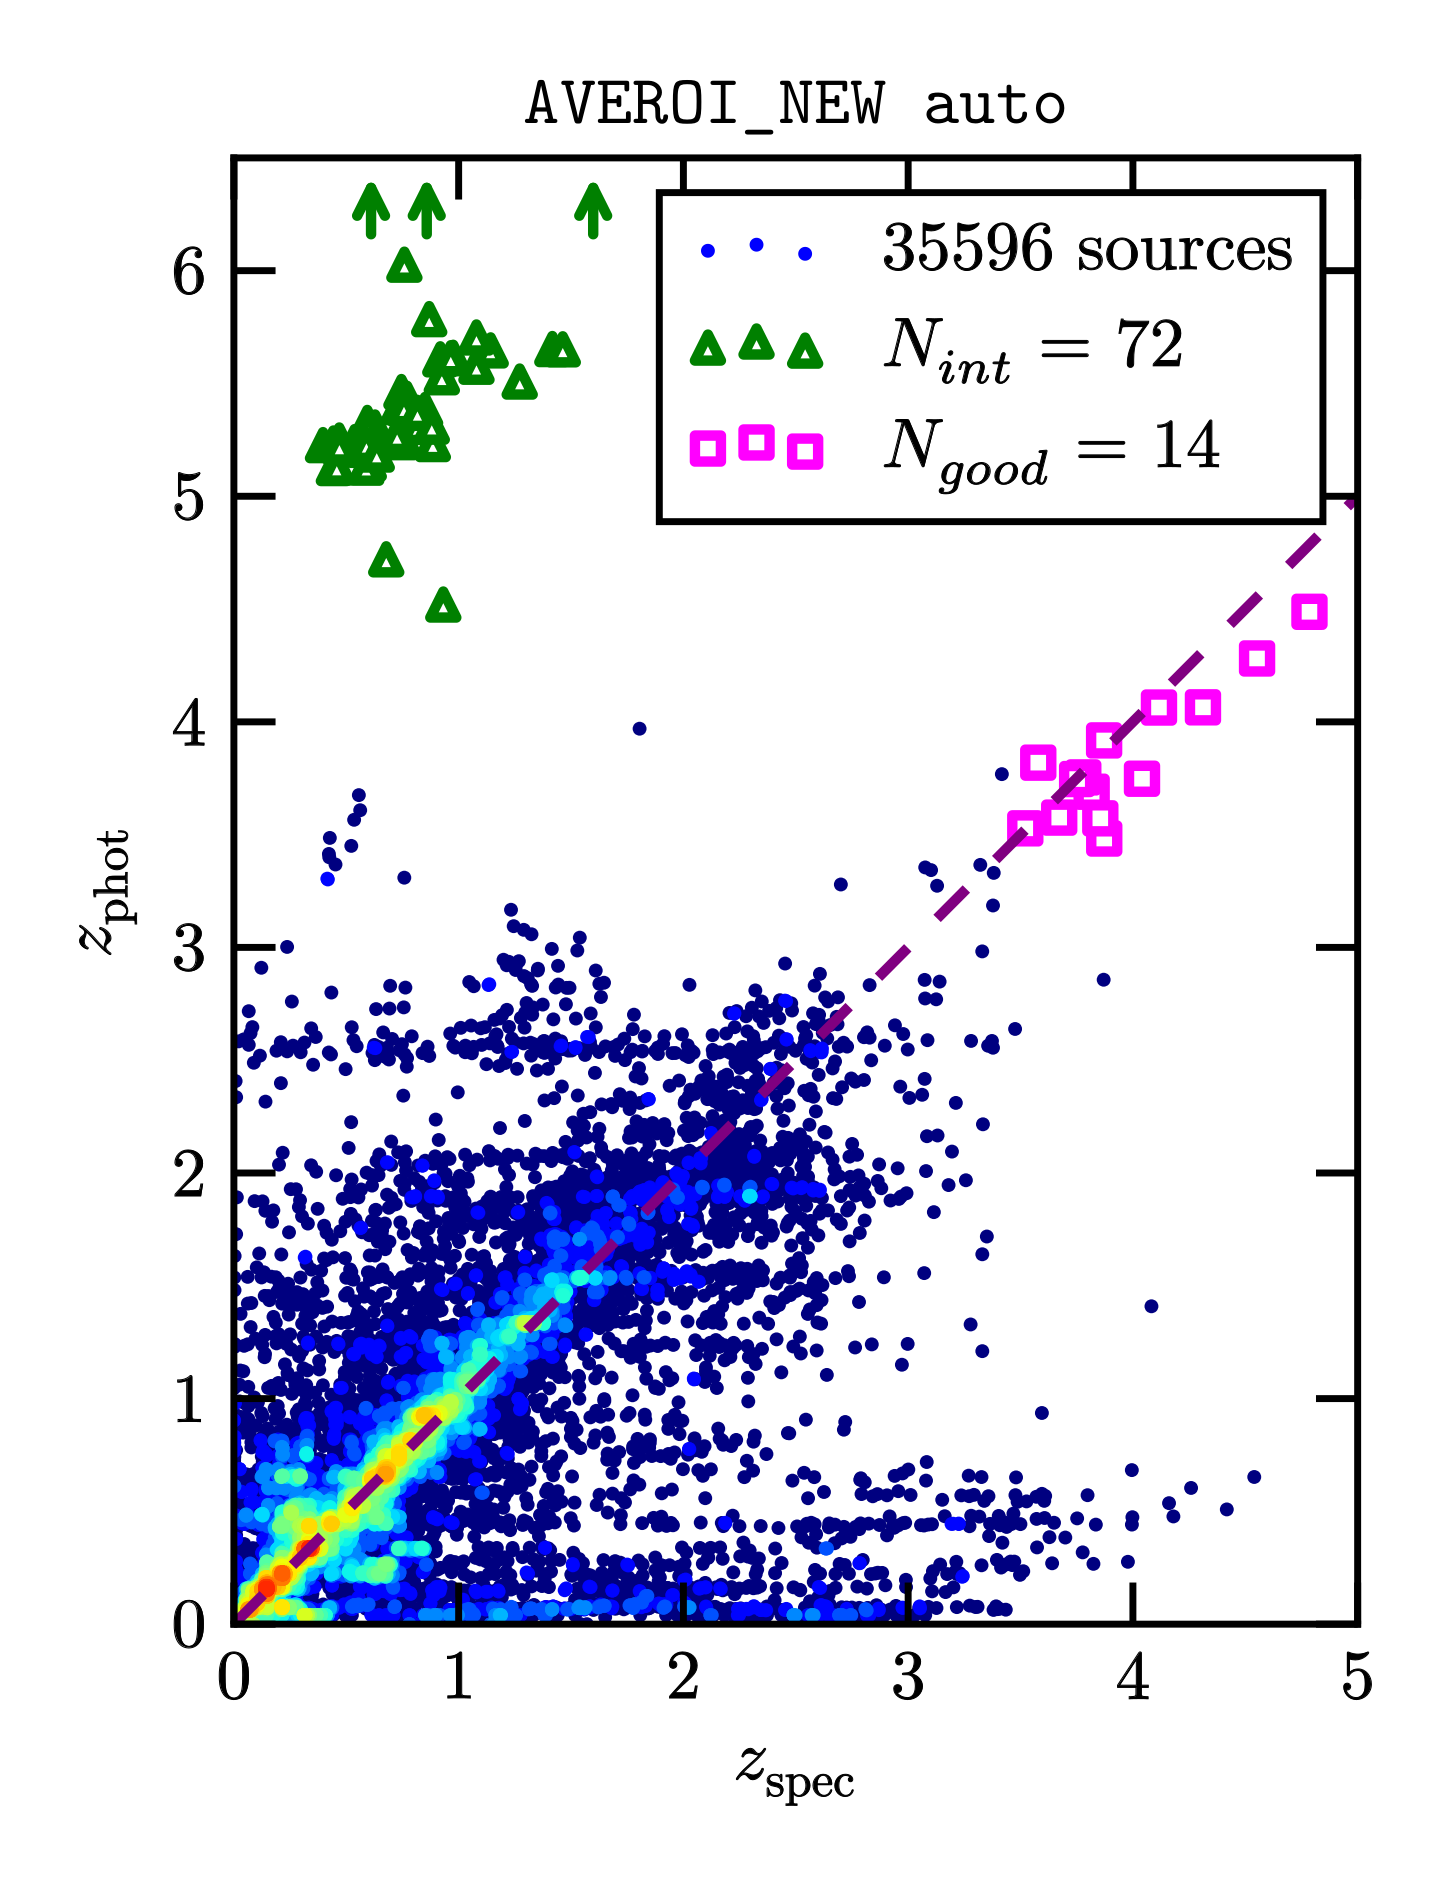
\includegraphics[clip, width=0.5\textwidth]{Chapter3/Figs/template_auto.png}}
\subfloat[]{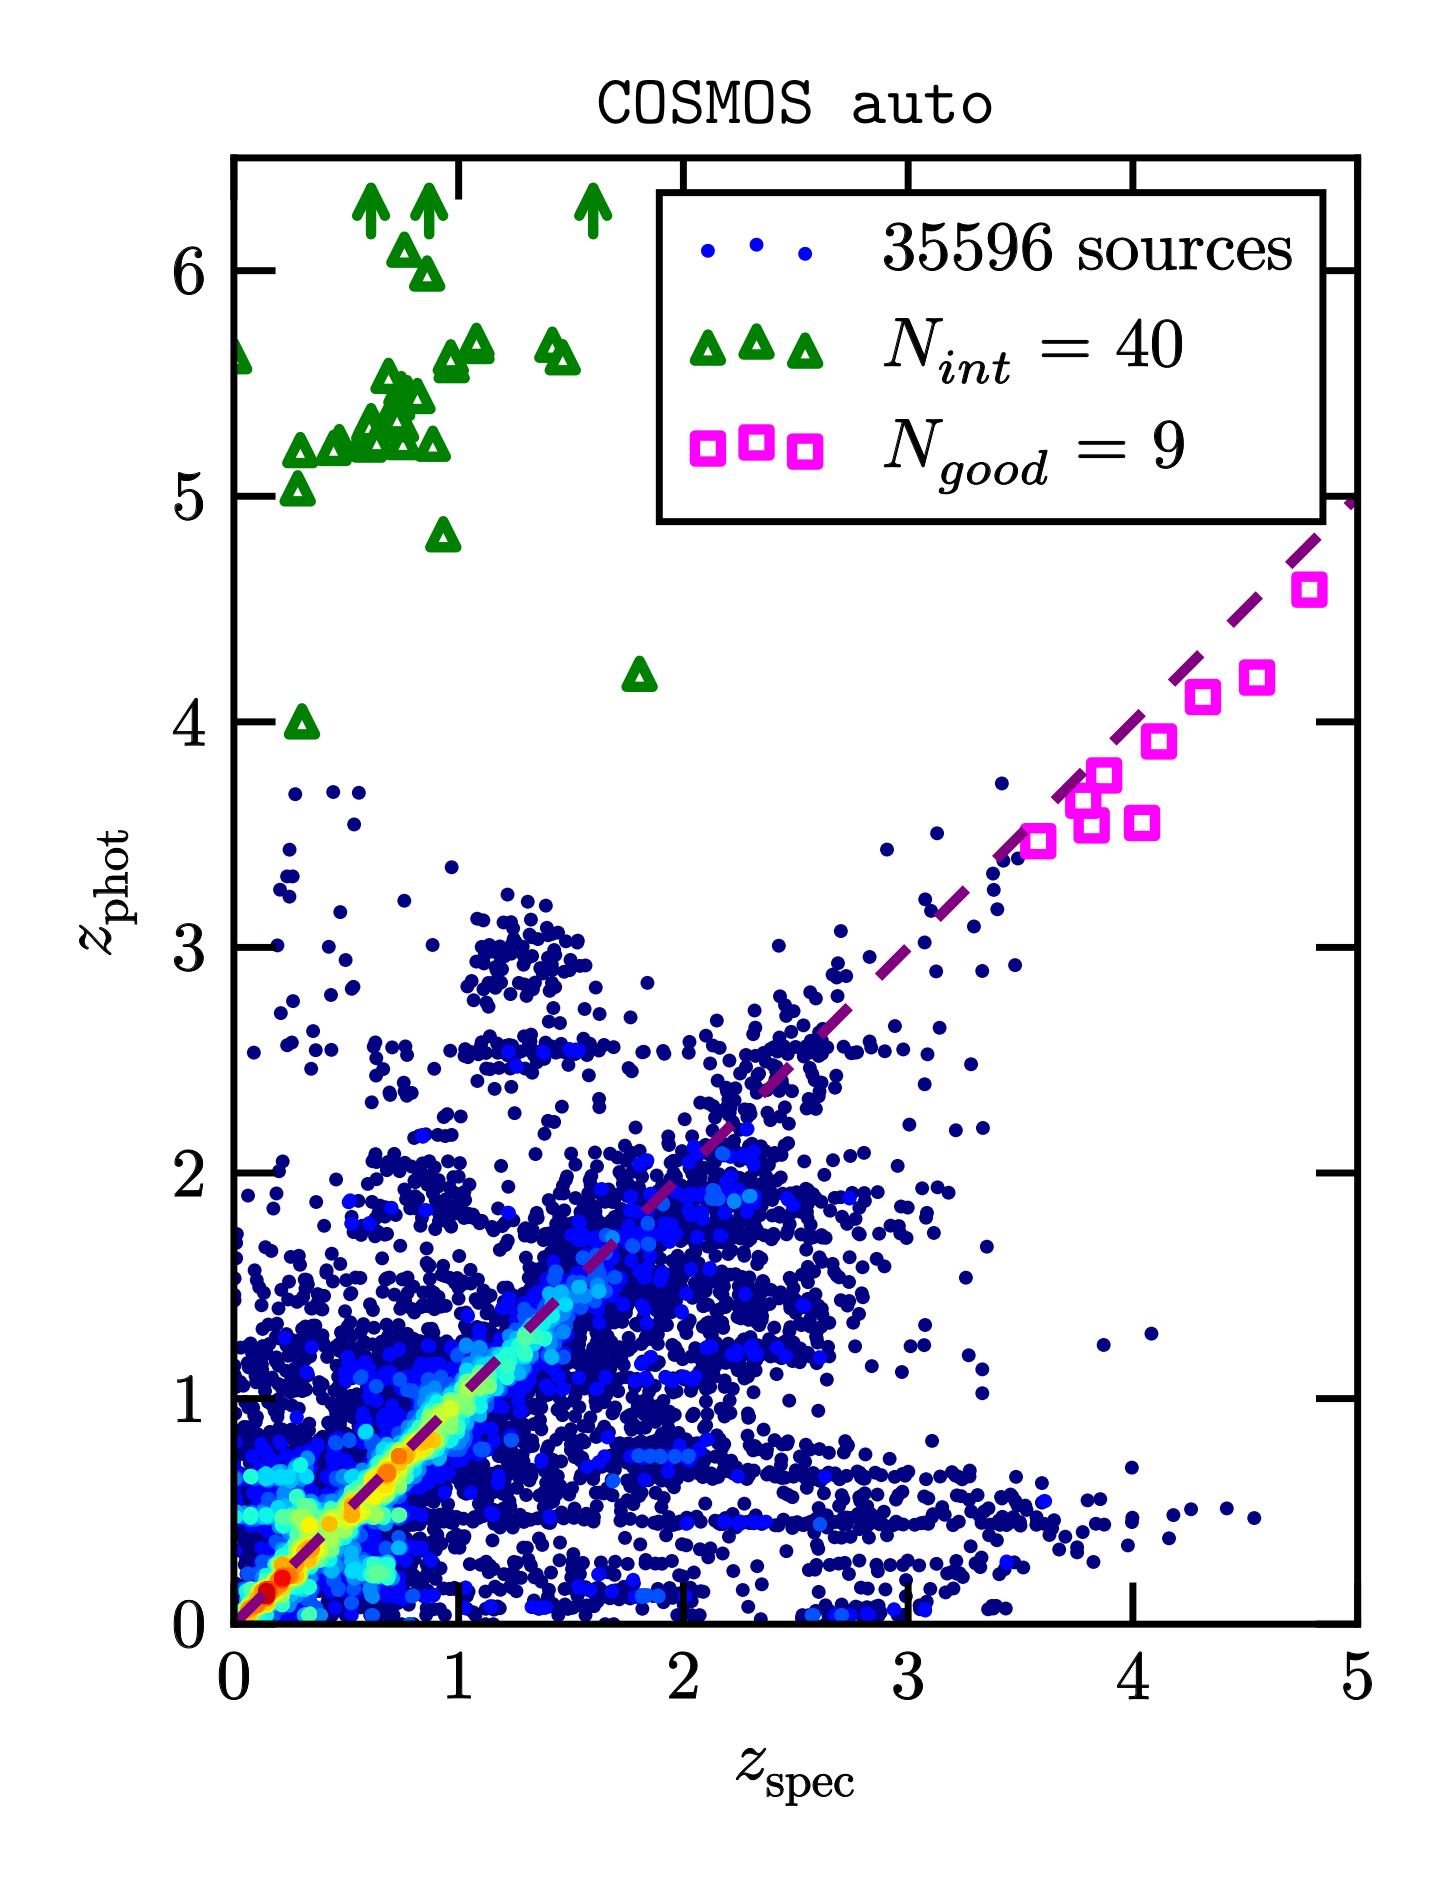
\includegraphics[clip, width=0.5\textwidth]{Chapter3/Figs/template_cosmos_auto.png}}
\caption{\textit{continued}}
\end{figure}

\begin{figure}
\ContinuedFloat
\subfloat[\label{fig:des_only}]{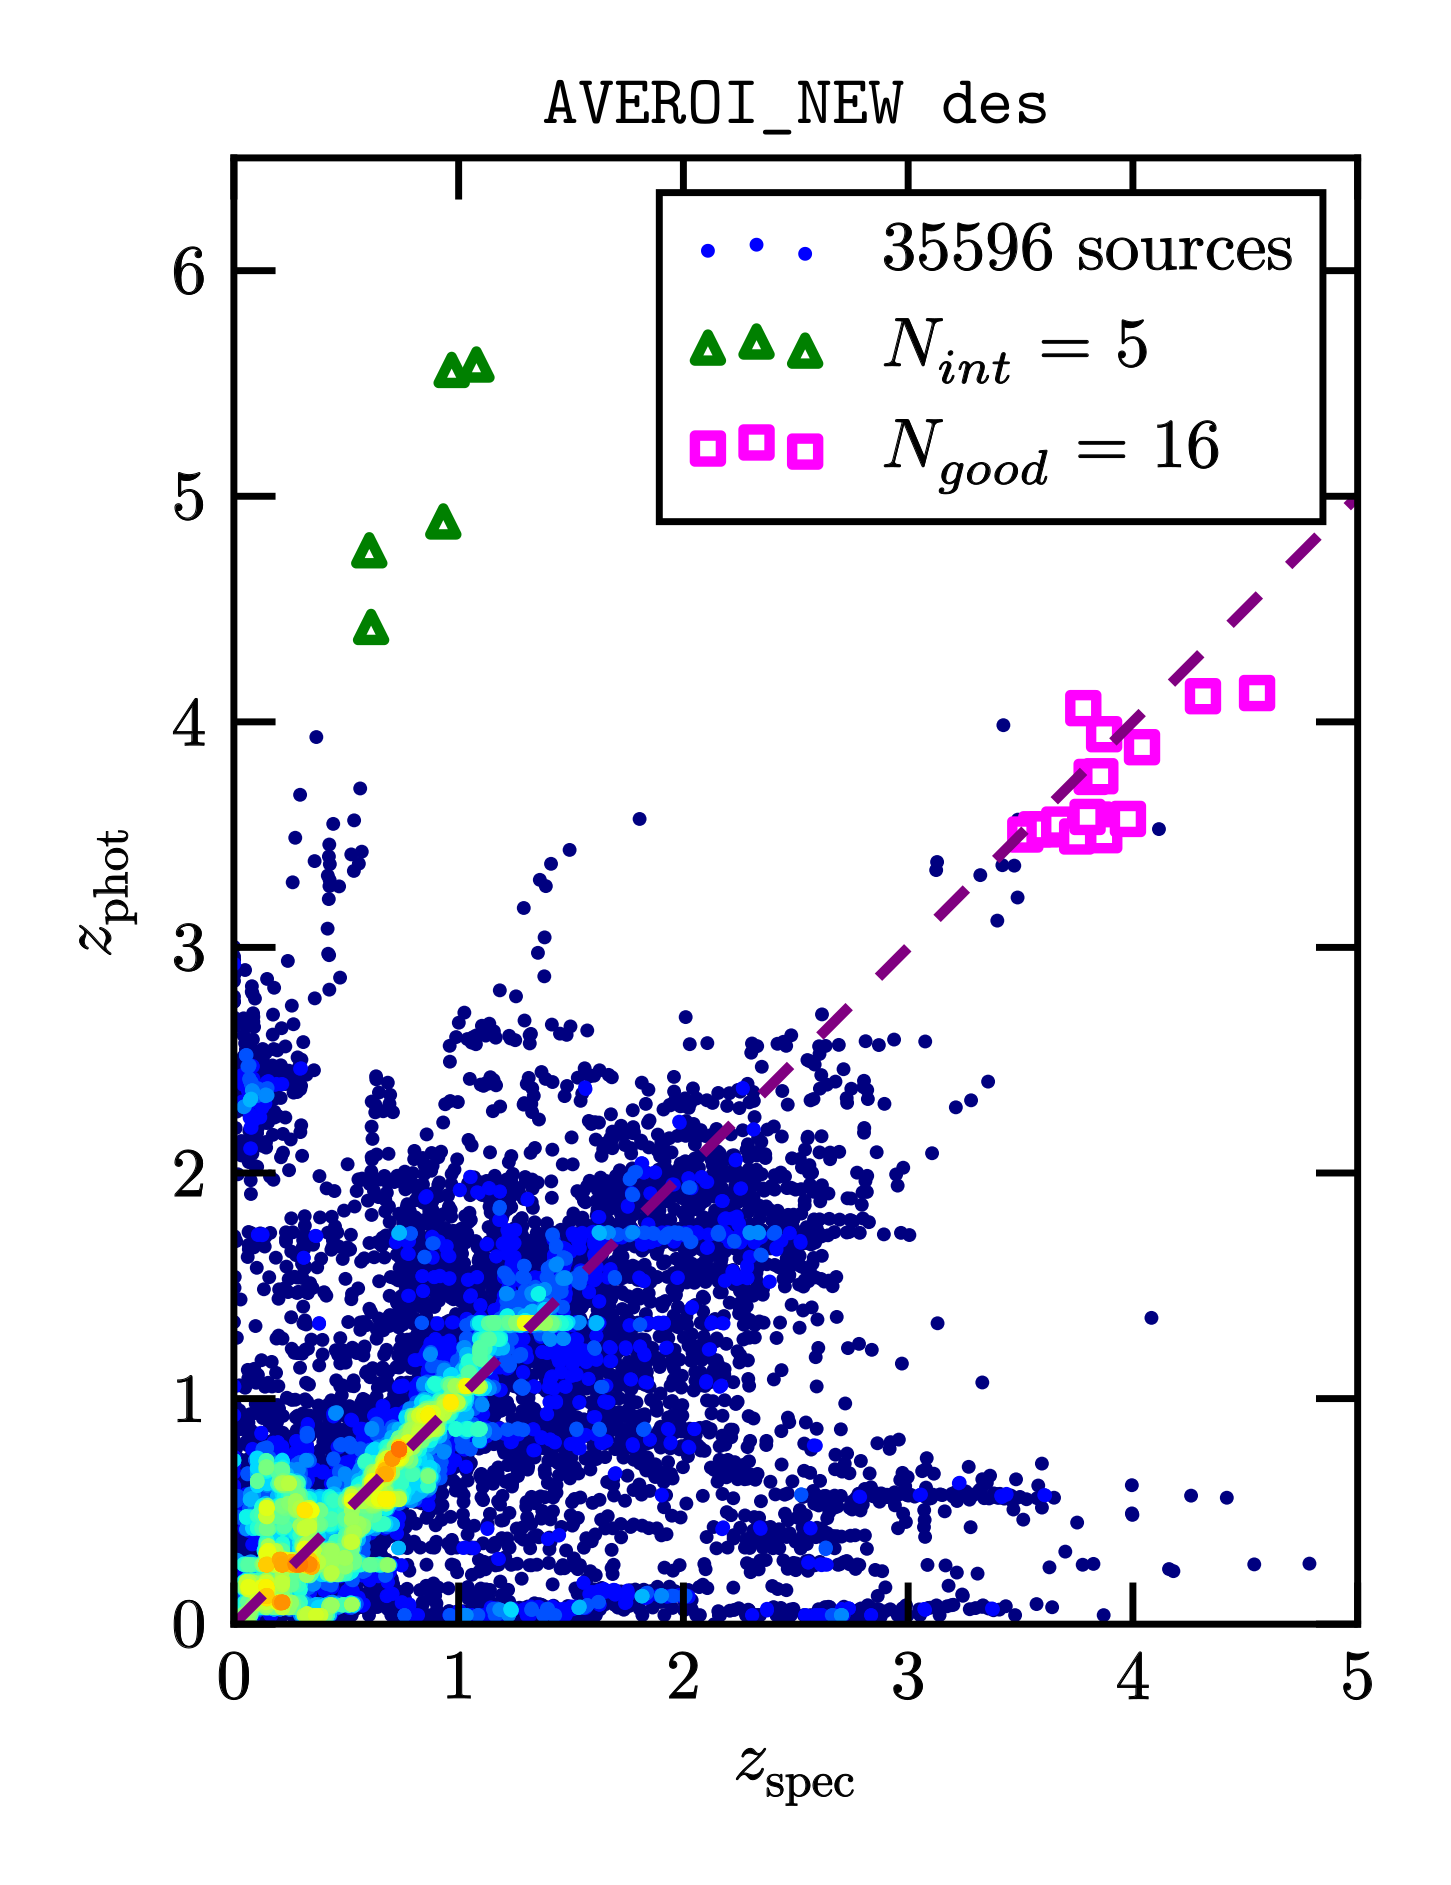
\includegraphics[clip, width=0.5\textwidth]{Chapter3/Figs/template_des_only.png}}
\subfloat[\label{fig:cosmos_des_only}]{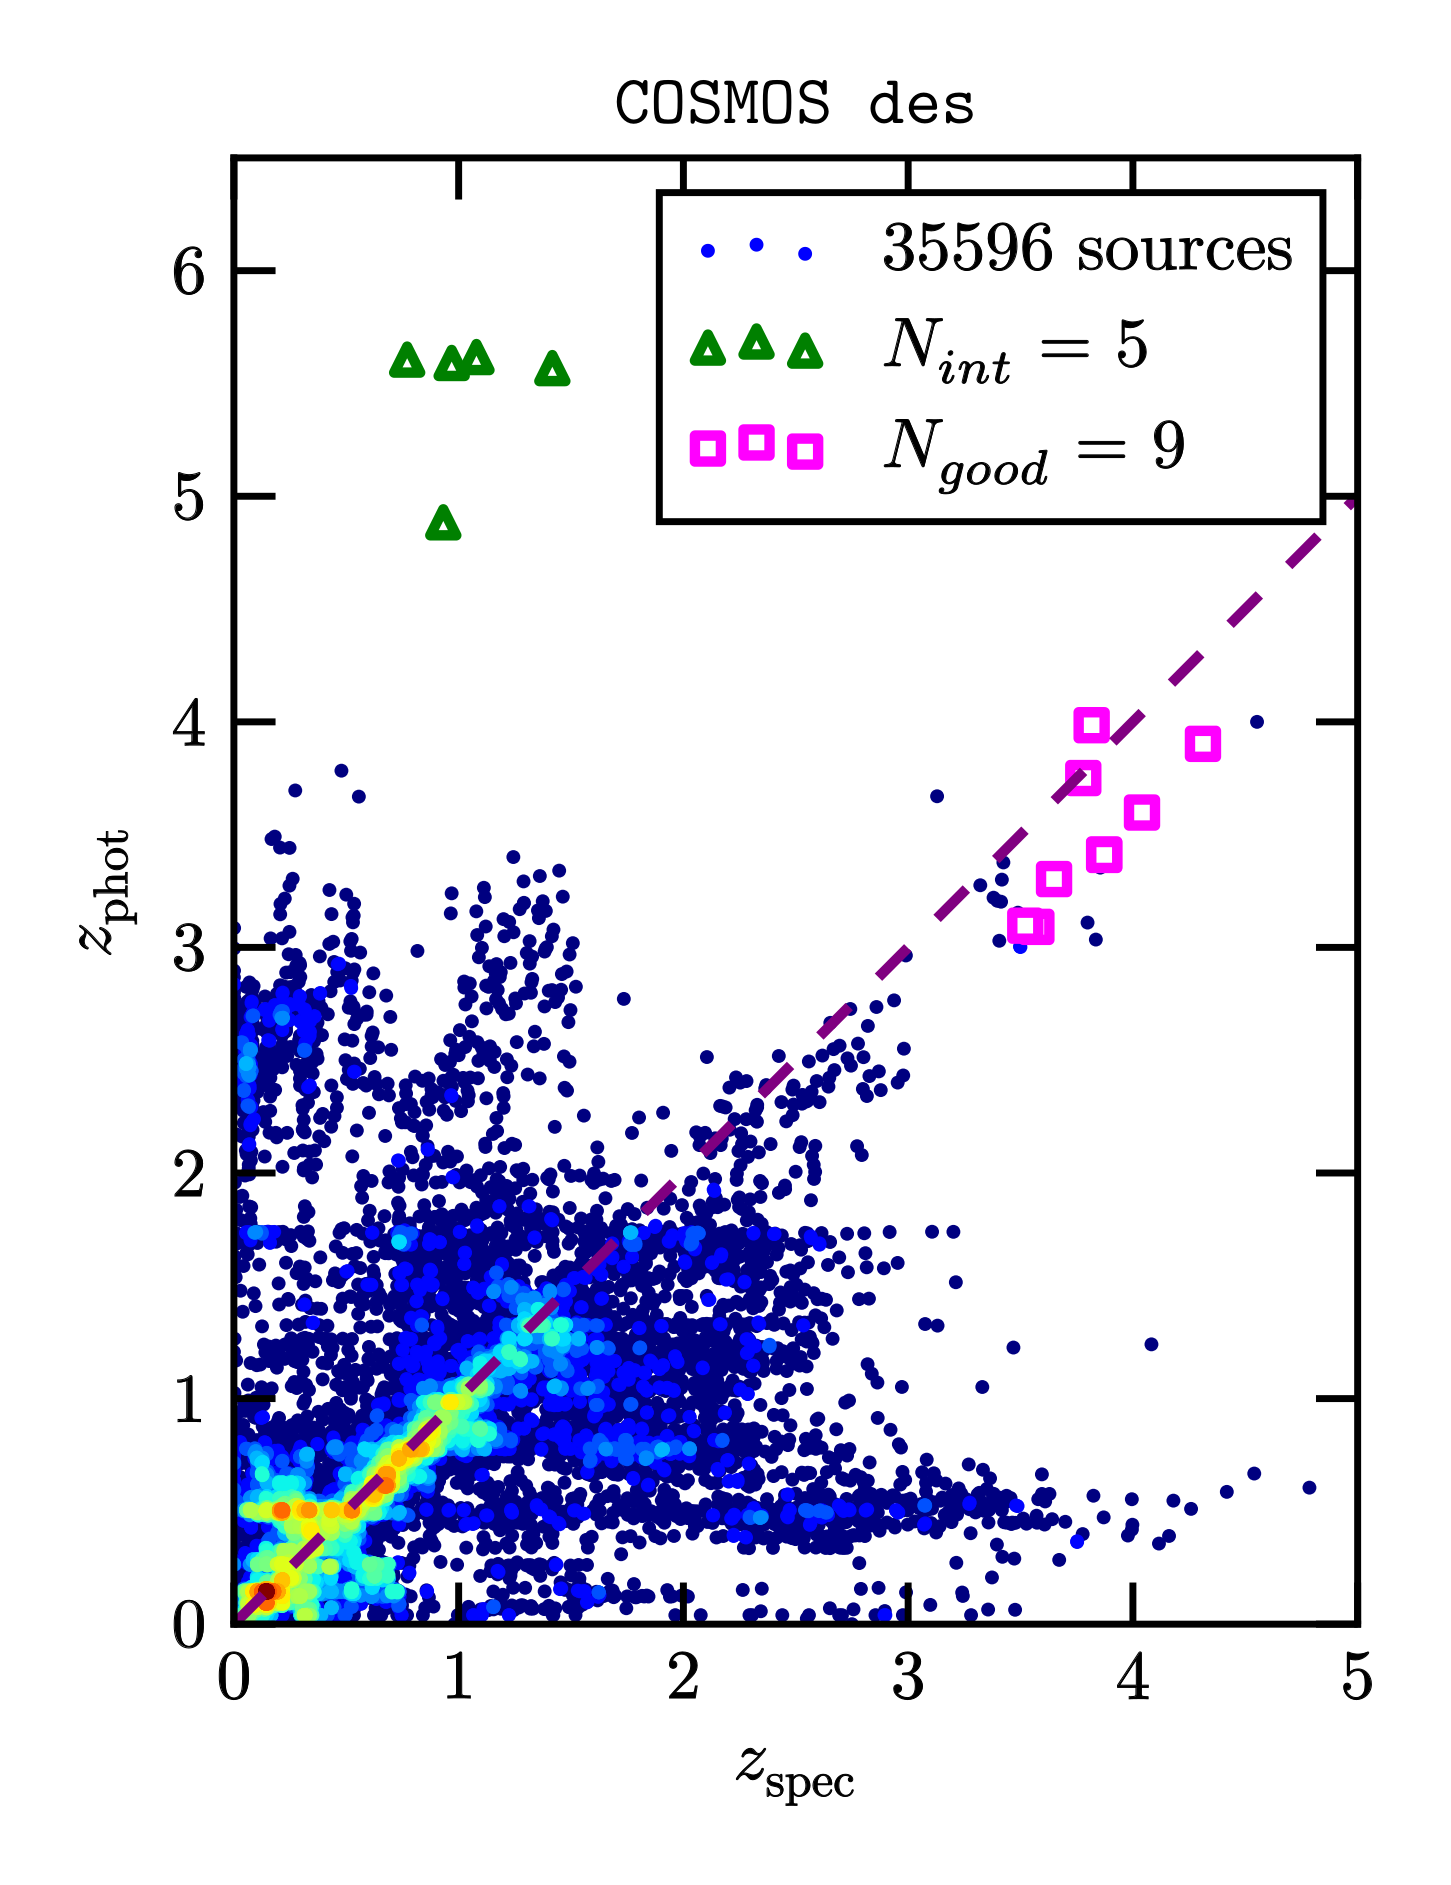
\includegraphics[clip, width=0.5\textwidth]{Chapter3/Figs/template_cosmos_des_only.png}}

\subfloat[]{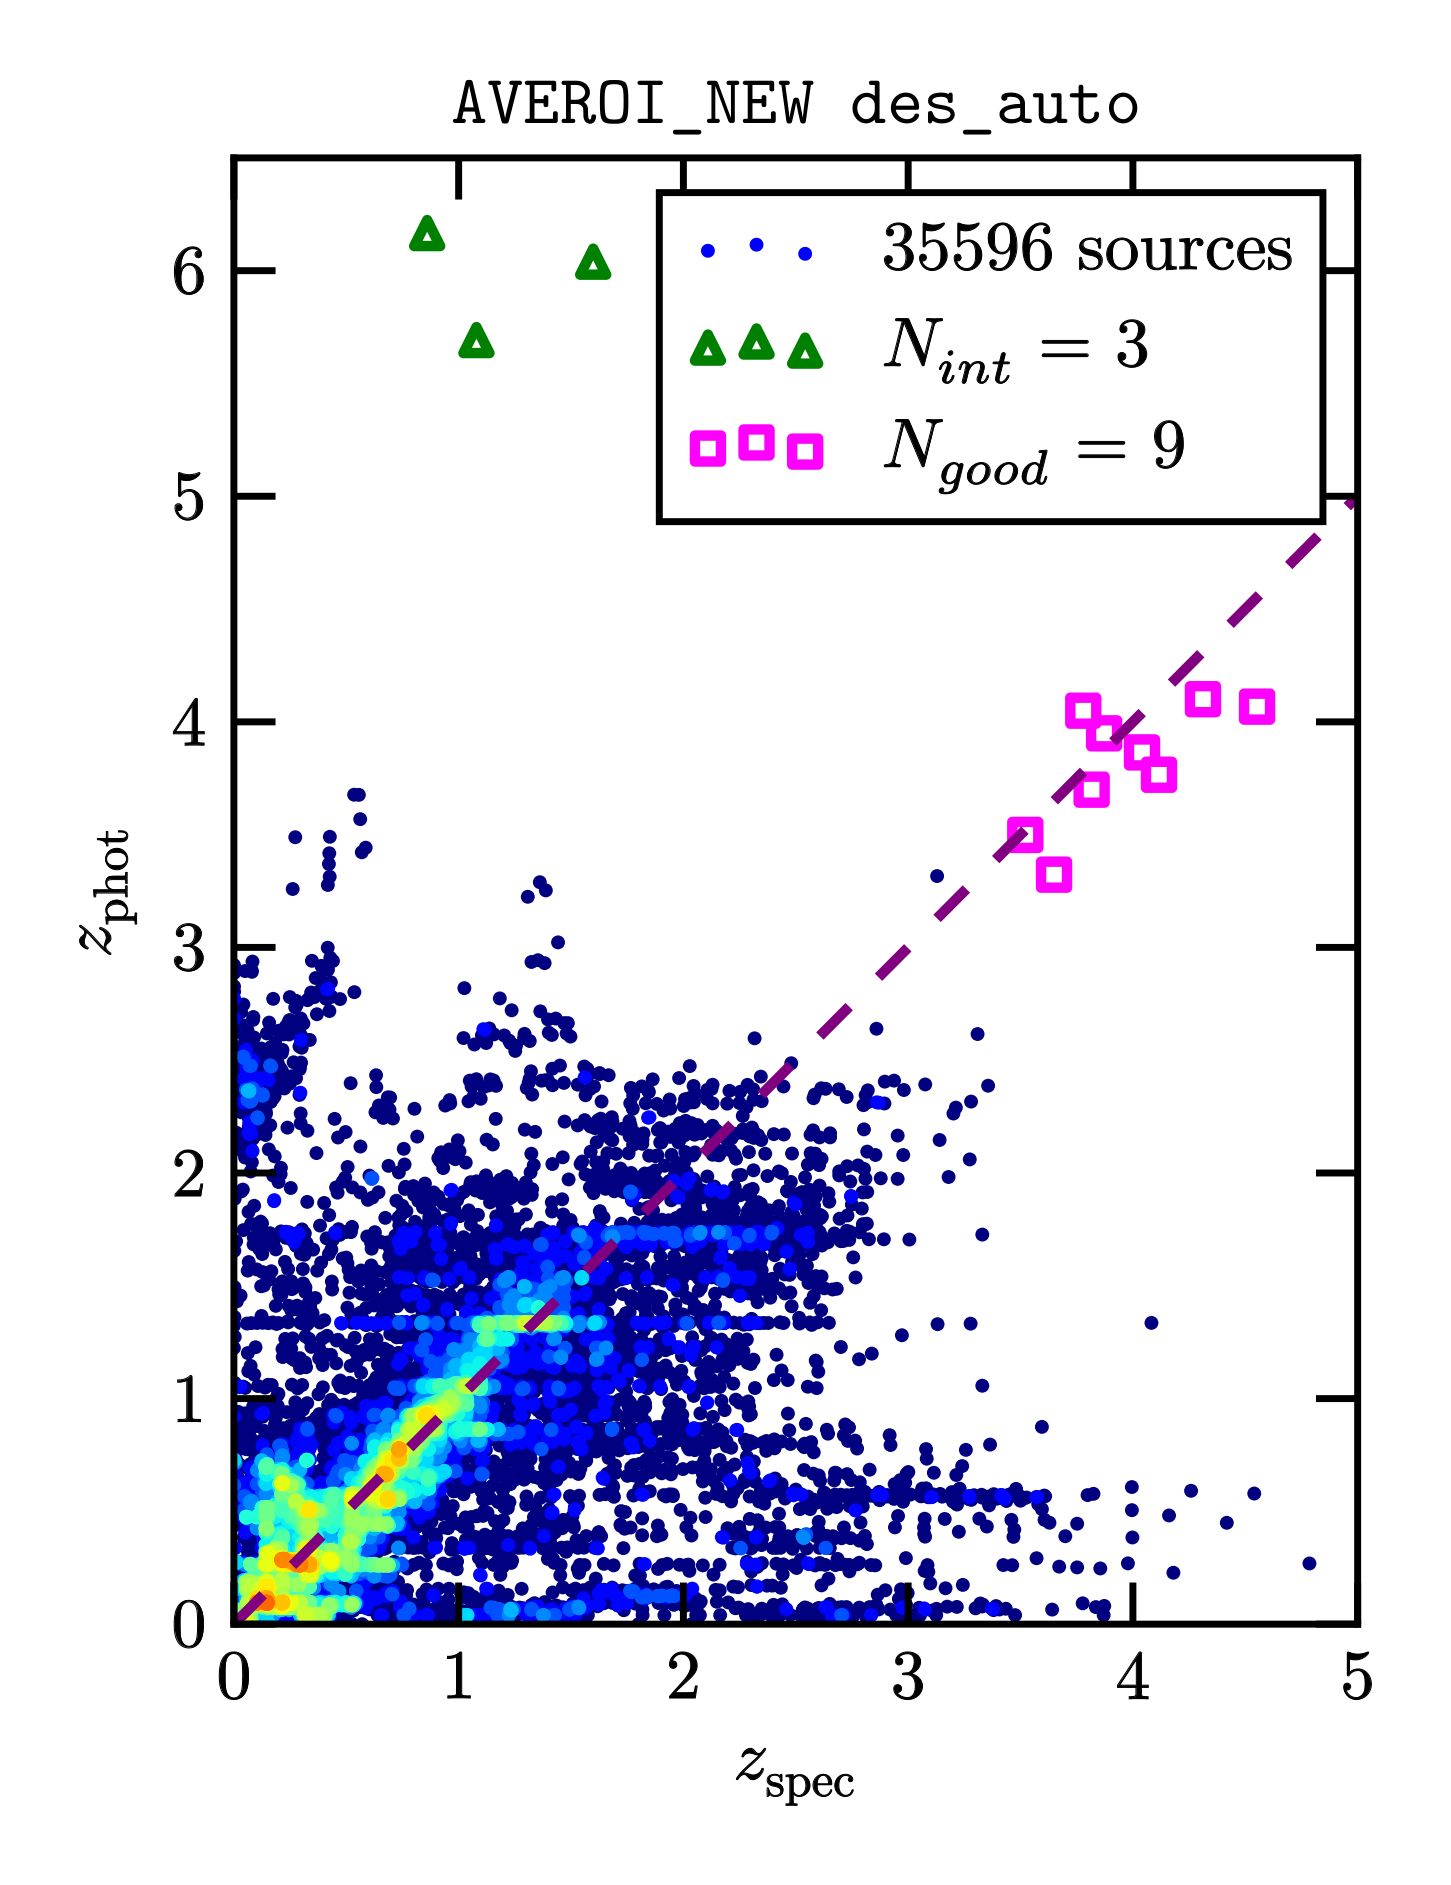
\includegraphics[clip, width=0.5\textwidth]{Chapter3/Figs/template_des_only_auto.png}}
\subfloat[]{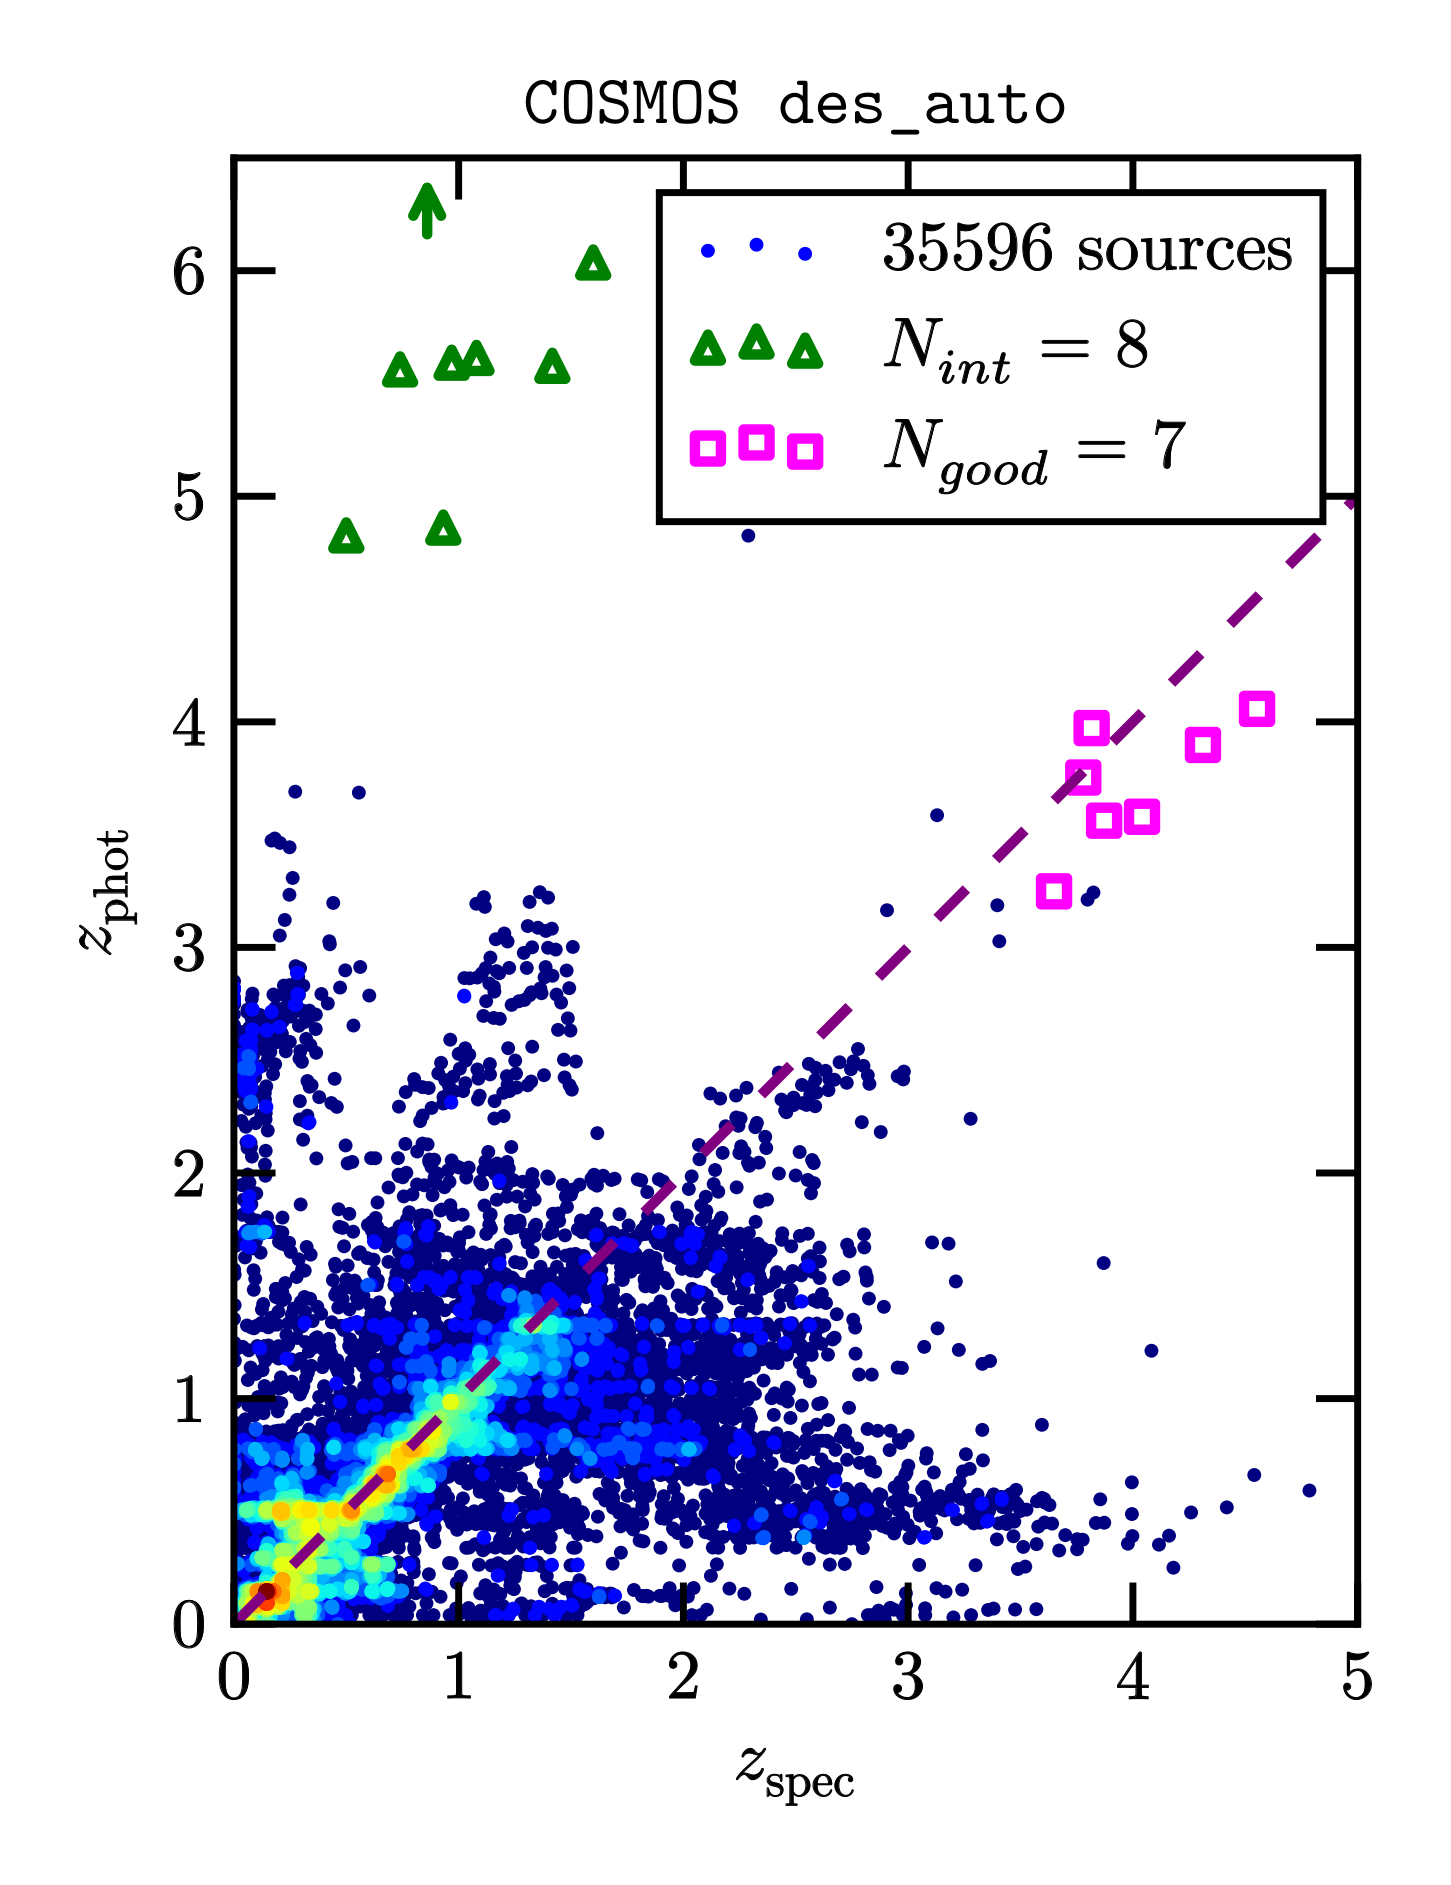
\includegraphics[clip, width=0.5\textwidth]{Chapter3/Figs/template_cosmos_des_only_auto.png}}
\phantomcaption
\end{figure}





\section{Discussion on configuration testing}\label{section:photoz_discussion}
The part of this chapter concerned with photometric redshift testing has now reached its final stage, where the preceding results can be used to explore the effect of all the different options that have been trialled. To this end, the current section will present a comparative evaluation of the photometric redshift performance for all the setups. In the analysis, configurations are compared by the values of their accuracy metrics in Table \ref{table:photoz_test} and by their photo-z distributions in Figure \ref{fig:photoz_distribution}. \par 

The end goal is to find the most suitable way to estimate photo-zs for the \DESVIDEO catalogue, which, as emphasised throughout this thesis, needs to be specifically geared towards optimal results at high redshifts.  At several points the discussion will also comment on the implication of the test results for general photo-z research. These analyses will disregard the high-redshift accuracy metrics, and looks only at those statistics that apply to the full testing sample --- i.e. the bias, scatter, and outlier fractions. Those primarily reflect the accuracy for the low-redshift ($z_{\mathrm{spec}}\lesssim1.5$) majority of galaxies in the sample, which is also approximately the range that most other photo-z studies tend to focus on.\par

%LOOK AT THIS TEXT BELOW
%As Section \ref{subsection:conclusion_photoz_intro} indicated at the start, one of the aims of this thesis is to utilise the \DESVIDEO dataset to investigate photo-z optimisation for the sake of future studies. Section \ref{section:photoz_discussion} has therefore analysed the general implications of the \DESVIDEO tests. This investigation looked only at the bias, scatter, and outlier fraction metrics, i.e. those that were measured on all objects in the testing sample. Naturally, these metrics thus primarily reflect the accuracy for the low-redshift ($z_{\mathrm{spec}}\lesssim1.5$) majority of galaxies in the sample, which is also the range at which most photo-z studies operate.



\subsection{Templates}
\subsubsection{Template sets}\label{subsubsection:template_sets}
In order to investigate which template set performs best, the \texttt{AVEROI\_NEW} and \texttt{COSMOS} entries in Table \ref{table:photoz_test} are compared directly for each setup\footnote{The \texttt{AVEROI\_NEW} \texttt{less\_ext} and \texttt{COSMOS} \texttt{ext} configurations are not directly comparable, because they use very different amounts of extinction. Therefore they are not considered in this template set comparison.}. A general observation is that the \texttt{COSMOS} templates perform better than the \texttt{AVEROI\_NEW} templates for most statistical measures and most configurations. The \DESVIDEO tests thus confirm the claim by \cite{2009ApJ...690.1236I} mentioned earlier in Section \ref{subsubsection:COSMOS}, that the \texttt{COSMOS} SEDs are generally more accurate than template sets based on the CWW spectra (such as the \texttt{AVEROI\_NEW} SEDs). \par


In terms of metrics, a notable exception is that the \texttt{AVEROI\_NEW} templates consistently show a larger value for $N_{\mathrm{good}}$ (except in the \texttt{des\_auto} setup where the values are identical). Secondly, the \texttt{AVEROI\_NEW} templates also perform better in terms of mean bias $\overbar{\Delta z}$ in all but one case (the \texttt{no\_prior} configuration being the exception). Regarding configurations, there are two instances where the \texttt{AVEROI\_NEW} templates are conclusively more accurate than \texttt{COSMOS}, namely the \texttt{des} and \texttt{des\_auto} setups. For the \texttt{des} setup, the mean and median bias $\overbar{\Delta z}$ and $\Delta z_{50}$ are 0.0120 and 0.0057 lower for the \texttt{AVEROI\_NEW} templates, and the $\sigma $, $f_{2\sigma}$, and $f_{3\sigma}$ values are 10.2\%, 13.7\% and 13.9\% lower. For the \texttt{des\_auto} configuration the metrics are lower by 0.0319 and 0.0242 for $\overbar{\Delta z}$ and $\Delta z_{50}$, and 13.2\%, 10.5\% and 16.4\% for $\sigma$, $f_{2\sigma}$ and $f_{3\sigma}$. A possible explanation for why the \texttt{AVEROI\_NEW} templates perform slightly better when using exclusively optical data might be found within Section \ref{subsubsection:COSMOS}. To recap, there it was stated that \cite{2009ApJ...690.1236I} claim that the better accuracy of the \texttt{COSMOS} templates is because they produce a better joining of the UV to the infrared. If this is indeed the reason why these SEDs perform better for the full \DESVIDEO filterset, it would follow that this advantage would not apply when only optical data is used. At the same time, the \texttt{AVEROI\_NEW} templates might be more reliable over visible wavelengths because that part of these spectra is based on the empirically measured CWW SEDs, whereas the \texttt{COSMOS} SEDs are theoretical. Furthermore, the CWW spectra are local, and the spectroscopic dataset used for the statistics is predominantly low-redshift. \par

Let us now return to the observation that the \texttt{COSMOS} templates generate superior statistics on the whole. Particularly interesting is the discovery that the \texttt{default} \texttt{COSMOS} setup produces better results than the \texttt{more\_ext} \texttt{AVEROI\_NEW} setup. Over the course of the following few sections, it will be demonstrated that those two are the best choice for their respective template sets. Upon comparing these configurations, the \texttt{COSMOS} metrics come out 0.0055 lower for $\Delta z_{50}$, and lower by 16.1\% in $\sigma$, 23.7 \% in $\sigma_{68}$, 0.8\% in $f_{2\sigma}$, and 10.2\% in $f_{3\sigma}$. The number of low-redshift interlopers $N_{\mathrm{int}}$ is also twice as small. The only instances where the \texttt{more\_ext} \texttt{AVEROI\_NEW} templates perform better is with regard to the mean bias $\overbar{\Delta z}$ (lower by 0.016), and the number of successfully retrieved high-redshift objects $N_{\mathrm{good}}$: the \texttt{COSMOS} setup correctly identifies only 14 high-redshift galaxies, whereas the \texttt{AVEROI\_NEW} results find 23. In the end, the latter advantage is one of the major reasons why the high-redshift search later in this thesis makes use of the \texttt{AVEROI\_NEW} templates. Section \ref{subsection:template_choice} will describe the reasons for this choice in detail. \par

The remainder of the setup comparisons will now determine the best configuration parameters for each template set. Such an analysis is useful both for finding the best way to apply each template set, and for a template-independent assessment of all the parameter options. The topic of template set choice will be revisited at the end in Section \ref{subsubsection:templates_revisited}.\par %TEMPLATE-INDEPENDENT COMPARISONS




\subsubsection{Extinction}\label{subsubsection:extinction_discussion}
The next point of inquiry involves the effects of dust extinction on the photo-zs. The observed trends with various amounts of extinction differ between the two template sets. To start with, the discussion will focus on the \texttt{AVEROI\_NEW} templates. It is evident from Table \ref{table:photoz_test} that the \texttt{default} setup with extinction values of up to $E(B-V)=1.0$ performs better than the \texttt{less\_ext} setup with a maximum extinction of only $E(B-V)=0.3$ (recommended in the \texttt{LePHARE} installation). The superior performance is demonstrated across $\overbar{\Delta z}$ (better by 0.0197), $\Delta z_{50}$ (0.0003), $\sigma$ (better by 9.0\%), $\sigma_{68}$ (10.3\%), $f_{2\sigma}$ (6.3\%), $f_{3\sigma}$ (9.0\%) and $N_{\mathrm{good}}$ (16 fewer interlopers). $N_{\mathrm{int}}$ is the only statistic where both setups are equally accurate. Specific reasons for this improvement can be found in Figure \ref{fig:basic} and Figure \ref{fig:less_ext}. The latter plot demonstrates that the \texttt{less\_ext} configuration contains a population of galaxies at $0\lesssim z_{\mathrm{spec}} \lesssim 1.5$ that are assigned high photo-zs of $z_{\mathrm{phot}}\gtrsim 2.5$. When inspecting the imaging and photometry for these sources, it becomes apparent that they are extremely red galaxies. It is likely that they are so red that without templates with adequate dust extinction the \SI{4000}{\angstrom} break at $z<1.5$ is mistaken for a \SI{1216}{\angstrom} Lyman break at $z>2.5$. However, when higher extinction values are included through the \texttt{default} setup, these galaxies are fitted well. The findings above thus suggest that the $E(B-V)\leq0.3$ dust extinction values listed in the \texttt{LePHARE} installation do not span the full range of attenuation observed in real galaxies. In fact, this shortcoming was partly implicitly acknowledged by the \cite{2007A&A...476..137A} study that the \texttt{AVEROI\_NEW} templates are derived from, which includes $E(B-V)$ values of up to 0.6. Nonetheless, the \DESVIDEO results indicate that this is also not sufficient --- out of a sample of 166 $z_{\mathrm{phot}}\gtrsim 2.5$ interloper galaxies that are poorly fitted by the \texttt{less\_ext} exctinction range, 16 are best fitted by templates as red as $E(B-V)=1.0$. This number is of the same order as the number of true high-redshift objects $N_{\mathrm{good}}=24$. This thesis therefore emphasises that it is important for high-redshift studies to include templates with large amounts of extinction, in order to accurately model very attenuated sources.\par 


%\begin{figure*}[!htpb]
%\centering
%\subfloat[]{
%	\includegraphics[clip, width=0.50\textwidth]{Chapter3/Figs/difference_basic.png}}
%\subfloat[]{
%	\includegraphics[clip, width=0.50\textwidth]{Chapter3/Figs/difference_less_ext.png}}
%\caption[]{}
%\label{fig:ext_difference}
%\end{figure*}


The \texttt{more\_ext} configuration is aimed at testing whether extinction values above $E(B-V)=1.0$ would further improve the photo-zs. Table \ref{table:photoz_test} shows that this is not the case for the spectroscopic testing sample, as the difference between the \texttt{default} and \texttt{more\_ext} metrics is negligible (the \texttt{default} results show only a marginal 0.0004 lower $\overbar{\Delta z}$, and any improvements are at the subpercent level for the $\sigma$, $\sigma_{68}$, $f_{2\sigma}$ and $f_{3\sigma}$ metrics). In fact, only 10 out of \num{35596} sources differed by more than 0.2 in photometric redshift across the two configurations. The two configurations could therefore be considered equivalent for the (low-redshift) population that dominates the spectroscopic subsample. Nevertheless, there is a potential benefit to including redder templates for the high-redshift search in the full catalogue, since extremely red galaxies are a common contaminant. As the statistical metrics indicate that there is no worsening performance when using the \texttt{more\_ext} setup, this potential advantage was considered a sufficient reason to regard the extinction values in the \texttt{more\_ext} as the optimal choice for the \DESVIDEO catalogue. \par 


The remaining analysis of the most suitable extinction values will now focus on the \texttt{COSMOS} templates.  When looking at the results for the \texttt{default} [$E(B-V)\leq0.5$], \texttt{ext} [$E(B-V)\leq1.0$] and \texttt{more\_ext} [$E(B-V)\leq2.0$] configurations, the conclusion is fairly straightforward: the photo-z metrics tend to worsen slightly with increased extinction ($\sigma$ and $f_{3\sigma}$ being the only exceptions). Overall this makes the extinction in the \texttt{default} setup the best choice for the \DESVIDEO data, although it must be noted that the differences between the three configurations are quite small ($<2\%$ for all metrics). The fact that the \texttt{default} setup performs best suggests that the extinction values of $E(B-V)\leq0.5$ in the default setup are largely sufficient, corroborating the values from \cite{2009ApJ...690.1236I} and the \texttt{LePHARE} \texttt{README} files. The optimal dust extinction required for the \texttt{COSMOS} SEDs is therefore less than for the \texttt{AVEROI\_NEW} templates, where values of up to $E(B-V)\leq1.0$ are needed to achieve the best performance. A likely explanation is that the \texttt{COSMOS} template set is either more complete or more accurate at the red end. In the latter case, this could again be related to the fact that the \texttt{COSMOS} templates provide a better joining of the UV to the IR than the \texttt{AVEROI\_NEW} templates, which leads to more accurate red SEDs. \par 


\subsubsection{Emission lines}\label{subsubsection:discussion_emlines}
%THE MOST PROMINENT RESULT IS THAT THERE ARE 4 MORE LOW REDSHIFT INTERLOPERS
To investigate the effect of adding emission lines, the metrics for the \texttt{no\_emlines} setups are compared to the \texttt{default} results. For the \texttt{COSMOS} templates, the statistics agree with the original findings by  \cite{2009ApJ...690.1236I}, which indicated that emission lines are important to the photo-z performance. The improvement in photometric redshifts is especially clear when comparing Figures \ref{fig:cosmos_basic} and \ref{fig:cosmos_no_emlines}. The most prominent enhancement occurs for the main body of objects below $z_{\mathrm{spec}}\lesssim1.2$, where the distribution is much narrower  with emission lines. In terms of metrics, the superior performance of the \texttt{default} setup is reflected in $\Delta z_{50}$ (lower by 0.0026); $\sigma$ (lower by 1.3\%); and particularly in $\sigma_{68}$ (36.8\%), which encapsulates the narrower distribution noted earlier. The \texttt{no\_emlines} configuration does perform better for $f_{2\sigma}$ (lower by 0.9\%) and $f_{3\sigma}$ (8.8\%), but because the $2\sigma$ and $3\sigma$ bounds are widened by the higher scatter $\sigma$, these lower outlier fractions do not directly correspond to better photometric redshifts. The \texttt{no\_emlines} results are also lower by 0.0124 in $\overbar{\Delta z}$, and indicate one more good high-z galaxy through $N_{\mathrm{good}}$, and one fewer low-redshift contaminant through $N_{\mathrm{int}}$. However, as the latter two metrics improve only by a single object, these advantages were deemed insignificant compared to the overall worse performance. Emission lines are therefore applied in the final \texttt{COSMOS} configuration. \par


The conclusions are more mixed for the \texttt{AVEROI\_NEW} templates. The most prominent result here is that there are 4 fewer low-redshift interlopers when emission lines are included. The \texttt{default} setup also shows slightly lower values of $\sigma$ (lower by 0.2\%) and $f_{3\sigma}$ (0.30\%), but it performs worse in terms of $\overbar{\Delta z}$ (higher by 0.0015), $\Delta z_{50}$ (0.0055),  $\sigma_{68}$ (higher by 2.36\%) and $f_{2\sigma}$ (0.32\%; although the last result again does not necessarily indicate worse emission line performance due to the narrower value of $\sigma$). Altogether, the \texttt{AVEROI\_NEW} results are therefore not clearly conclusive for photometric redshift research in general. However, the lower values of $\sigma$, $f_{3\sigma}$, and particularly the lower number of low-redshift contaminants, make the application of emission lines the most suitable choice at high redshifts.\par 


%Regarding emission lines, the statistics in this thesis agree with the original findings by  \cite{2009ApJ...690.1236I}, which indicated that emission lines are important to the photo-z performance. The improvement is relatively subtle for the \texttt{AVEROI\_NEW} templates. The most prominent result is that the \texttt{no\_emlines} setup includes 4 more low redshift interlopers than the \texttt{default} configuration. The \texttt{default} setup also performs a little bit better in $\overbar{\Delta z}$ (lower by 0.0015), $\Delta z_{50}$ (0.0055), $\sigma$ (lower by 0.2\%), $f_{2\sigma}$ (0.32\%) and $f_{3\sigma}$ (0.30\%). $\sigma_{68}$ is the only statistic that is better without emission lines (by 2.36\%).

%THEY WILL BE INCLUDED
%\paragraph{} Because the results for both template sets indicate that the inclusion of emission lines improves the photometric redshifts, they are included in the final best setups.  {\color{red} revisit this to streamline with the story in this section}

%EMISSION LINES AT HIGH-Z https://ui.adsabs.harvard.edu/abs/2010A%26A...515A..73S/abstract

%\paragraph{} {\color{red}Because the inclusion of emission lines indeed improves the photo-z performance, this feature was included in the final selected setups. }

\subsection{Photo-z code options}
\subsubsection{Prior}\label{subsubsection:discussion_prior}
%THESE OUTCOMES CAN BE DISCARDED
When comparing the \texttt{default} and \texttt{no\_prior} setups, it is clear that the $N(z)$ prior indeed functions as expected. Based on Table \ref{table:photoz_test}, the use of such a prior improves the scatter $\sigma$ and $\sigma_{68}$ by 9.2\% and 4.8\% respectively for the \texttt{AVEROI\_NEW} templates, and by 8.9\% and 3.8\% for the \texttt{COSMOS} SEDs. It is noteworthy that a fall in scatter indeed agrees with previous studies by \cite{2006A&A...457..841I} and \cite{2015ApJ...801...20T}. Regarding outlier fractions, even though the $f_{2\sigma}$ and $f_{3\sigma}$ values come out lower without a prior, those outcomes probably do not reflect a true worsening in redshifts because the lower values are likely caused by the higher scatter $\sigma$. There seems to be no clear trend in improvement with regards to the mean and median bias $\overbar{\Delta z}$ and $\Delta z_{50}$. For the \texttt{AVEROI\_NEW} templates, the inclusion of a prior improves $\overbar{\Delta z}$ by 0.0122, but $\Delta z_{50}$ gets slightly worse by 0.0009. On the other hand, for the \texttt{COSMOS} templates the prior improves $\Delta z_{50}$ by 0.001, but $\overbar{\Delta z}$ gets worse by 0.0132. \par



More insights into the effects of a prior can be obtained by direct comparisons between Figure \ref{fig:basic} and Figure \ref{fig:no_prior} (for \texttt{AVEROI\_NEW}), and between Figure \ref{fig:cosmos_basic} and Figure \ref{fig:cosmos_no_prior} (for \texttt{COSMOS}). In both cases, the plots without a prior show an outlier population of galaxies with $z_{\mathrm{spec}}<1$ and $z_{\mathrm{phot}} > 2.5$, which is strongly reduced with the inclusion of a prior. In particular, the prior decreases the number of problematic fits at $z_{\mathrm{phot}} \sim 3$ for which the \SI{4000}{\angstrom} break at $z\sim 0$ is confused with a Lyman break at $z\sim 3$, in agreement with predictions by \cite{2000ApJ...536..571B}. The reduction of outliers is also reflected numerically in the lower values of $N_{\mathrm{int}}$: compared to the \texttt{no\_prior} configurations, the \texttt{default} setups contains 71 fewer interlopers for the \texttt{AVEROI\_NEW} templates and 54 fewer for the \texttt{COSMOS} templates. This corresponds to a reduction by a factor 1.5 and 2 respectively. The result that a prior cuts down extreme outliers mirrors similar findings by e.g. \cite{2000ApJ...536..571B}, \cite{2006A&A...457..841I}, and \cite{2015ApJ...801...20T}.\par

The improved accuracy provided by the prior does come at a cost, as its application is found to reduce the number of good high-redshift galaxies $N_{\mathrm{good}}$. The difference is relatively small for the \texttt{AVEROI\_NEW} configuration ($N_{\mathrm{good}}$ is 4 less), but it is significant for the \texttt{COSMOS} templates, where $N_{\mathrm{good}}$ is reduced by 12 objects. This suggests that the inclusion of a prior excludes true high-redshift sources from a photometrically selected sample, in agreement with predictions by \cite{2000ApJ...536..571B}. Despite this disadvantage, it was nevertheless decided to include a prior in the final photo-z setup. The reasons for this decision are two-fold. Firstly, the fractional reduction in contamination by including a prior is larger than the loss of good sources, and given the rarity of true high-redshift galaxies it is important to reduce the contamination. Secondly, the spectroscopically confirmed sources in the photo-z tests are biased towards bright sources for which spectra can be measured easily. The effect of low-redshift interlopers in a real catalogue with many faint objects is expected to be much larger. Including a prior will help to limit this contamination.\par  


%REWRITE THIS TO BE IN LINE WITH THE CONCLUSION
\subsubsection{Adaptive offsets}
The adaptive offsets also appear to be working as expected, since the tests show that they generally improve the photo-z statistics. These improvements particularly concentrate in the scatter and outlier fractions, a result which was previously also found by \cite{2013ApJ...775...93D}. For the \texttt{AVEROI\_NEW} templates, the \texttt{default} setup performs better than the \texttt{no\_adapt} setup in terms of $\overbar{\Delta z}$ (although only marginally by 0.00001), $\sigma$ (by 5.8\%), $\sigma_{68}$ (23.3\%), $f_{2\sigma}$ (0.6\%), $f_{3\sigma}$ (4.7\%), $N_{\mathrm{int}}$ (14 fewer interlopers) and $N_{\mathrm{good}}$ (1 more high-z galaxy). The only exception is $\Delta z_{50}$, which improves by 0.0019 without the adaptive offsets. Although less prominent, a general improvement is also seen for the \texttt{COSMOS} templates, where the \texttt{default} configuration shows improvement compared to the \texttt{no\_adapt} setup in $\sigma$ (by 3.6\%), $\sigma_{68}$ (39.2\%) and $f_{3\sigma}$ (2.5\%). On the other hand,  $\overbar{\Delta z}$ and $\Delta z_{50}$ are better without adaptive offsets, by 0.0066 and 0.0096 respectively. $f_{2\sigma}$ is also 0.9\% lower, although this result is inconclusive as to the real redshift improvement because of the higher value of $\sigma$. A further advantage of the \texttt{no\_adapt} \texttt{COSMOS} setup, especially relevant to this thesis, is that without the adaptive offsets, the number of interlopers $N_{\mathrm{int}}$ goes down by 3, and $N_{\mathrm{good}}$ goes up by 3. Given the goal of producing optimal results at high redshifts, this could prima facie be considered a reason not to use the offsets with the \texttt{COSMOS} templates. However, the noted improvements are fairly small, and the lower scatter values, together with a comparison between Figure \ref{fig:cosmos_no_adapt} and Figure \ref{fig:cosmos_basic}, all indicate that the adaptive offsets do generally improve the redshifts. The plots show slight improvement around $z_{\mathrm{phot}}\sim3$, whilst the main enhancement is concentrated around $z_{\mathrm{phot}}<0.5$. Even though those lower redshifts are not directly relevant for the high-redshift performance, the positive effect of the offsets suggests that the adaptive corrections track real properties, which would generally be expected to translate to high redshifts too. For all the reasons mentioned above, it was therefore decided to include the adaptive offsets in the final selected configuration for both setups. \par

It must be borne in mind, however, that improvements in photo-z performance when applying adaptive offsets are trivially expected if these offset corrections have been calibrated via the same set of spectroscopic objects that was used in the photo-z accuracy tests (as is the case in this thesis). When using such corrections to estimate photometric redshifts for a larger superset of survey objects, the measured advantage does therefore not necessarily carry over. Because offset values can be affected by template incompleteness (see Section \ref{subsection:adaptive_offsets}), they may be biased towards the types of galaxies present within the spectroscopic subsample. If these sources are not representative of the galaxy population in the full survey, the offsets may not improve the photo-z performance for the total \DESVIDEO catalogue. Fortunately, the spectroscopic sample in this thesis is large and originates from a varied range of sources, making it likely that the spectra are indeed varied enough to avoid strong biases. Furthermore, the adaptive offsets also correct for errors in the zero-point calibration as well as aperture corrections, both of which are independent of the spectroscopic subsample. At least some of the improvements provided by the adaptive offsets are therefore expected to apply directly to the full survey, justifying the decision to include this feature in the final configurations. \par



\subsection{Input photometry}
\subsubsection{Auto vs aperture fluxes}\label{subsubsection:auto_magnitudes}
The analysis will now turn to the question of whether auto or aperture fluxes produce more accurate photometric redshifts. For the \texttt{COSMOS} templates, Table \ref{table:photoz_test} shows that the aperture fluxes in the \texttt{default} setup perform better than the auto fluxes in the \texttt{auto} setup for almost all metrics. Improvements were observed in $\overbar{\Delta z}$ (lower by 0.0286), $\Delta z_{50}$ (0.0080), $\sigma$ (lower by 4.2\%), $\sigma_{68}$ (12.4\%), $f_{2\sigma}$ (8.3\%), $f_{3\sigma}$ (1.3\%) and $N_{\mathrm{good}}$ (5 more objects). The only exception is $N_{\mathrm{int}}$, which is lower by 12 objects when adopting auto photometry. \par


For the \texttt{AVEROI\_NEW} templates, aperture fluxes also produce better results for $\overbar{\Delta z}$ (lower by 0.0139), $\sigma_{68}$ (lower by 12.7 \%), $f_{2\sigma}$ (1.0\%; although this is insignificant due to the worse performance in $\sigma$, see below) and $N_{\mathrm{good}}$ (9 more objects). However, the auto fluxes perform better in terms of $\Delta z_{50}$ (by 0.0067), $\sigma$ (2.2\%), $f_{3\sigma}$ (1.0\%) and $N_{\mathrm{int}}$ (33 fewer interlopers). A possible explanation for why some metrics improve under the \texttt{auto} setup may be to do with the sizes of some objects. For extended sources larger than \SI{1.95}{\arcsec}, \SI{1.95}{\arcsec} apertures cannot capture their full emission, whereas auto apertures --- which are scaled individually to the size of each source --- are expected to produce more accurate estimates of their total flux. Since photometric redshifts predominantly\footnote{For the sake of conceptual clarity, the effect of the $N(z)$ prior is set aside in this line of reasoning.} rely not on the absolute flux measurement but on the colour \textit{difference} between filters, using fixed aperture photometry is generally not a problem for most sources (as reflected in the fact that the photo-zs still work well for the vast majority of large objects). Nevertheless, it can occasionally be an issue for extended objects where different regions have different colours, or if the DES and VIDEO astrometry do not line up perfectly\footnote{Even though the astrometry of the two surveys was found to line up very well (see Section \ref{subsection:astrometry}), for extended objects that are bright outside the aperture, even a small offset could make a difference.}. The use of aperture fluxes could thus occasionally lead to catastrophic photo-z failures, which would particularly manifest in higher $\sigma$ scatter and larger outlier fractions compared to the auto statistics, while leaving the $\sigma_{68}$ scatter in the very core of the distribution mostly unaffected. This behaviour is indeed exactly what is detected in the measurements of $\sigma$, $\sigma_{68}$, and $f_{3\sigma}$ of the \texttt{AVEROI\_NEW} configuration. It is not clear to the author why the partial improvement with auto photometry is only observed for that template set. It is speculated that the answer probably lies in the specifics of the SEDs, possibly combined with the effect of the adaptive offsets (which are different for each setup). Nevertheless, for the \texttt{COSMOS} setup the aperture fluxes do show smaller improvements for $\sigma$, $f_{2\sigma}$, and $f_{3\sigma}$ than for $\sigma_{68}$ compared to the auto photometry, in line with the hypothesis that adopting auto fluxes has a larger impact on the catastrophic failure rate than on the main body of photo-zs. \par


The reasoning above can also explain why for both template sets the \texttt{auto} results show lower values for $N_{\mathrm{int}}$. The author visually inspected\footnote{The general process for the visual inspection of photo-z fits will be described in more detail in Section \ref{subsection:visual_inspection}.} the imaging and best-fit SEDs  of low-redshift interlopers in the \texttt{default} setups, and found that the majority of these objects are very red extended galaxies. As explained, auto magnitudes capture more of the total flux for such large sources, altogether making it less likely that the code assigns them erroneous (in this case high) redshifts. However, one must note that with values of 72 (\texttt{AVEROI\_NEW}) and 40 (\texttt{COSMOS}), $N_{\mathrm{int}}$ is not close to zero even when applying auto photometry, so using these fluxes still cannot properly eliminate low-redshift contamination from extended objects. This is probably partly caused by template incompleteness at the very red end, and partly by the fact that the forced photometry in this thesis bases the position of the auto apertures on the shape of an object in the $r+i+z$ detection image. For galaxies that are more extended in VIDEO than in DES, such apertures would still be too small to capture the full flux. \par


Despite creating less contamination at high redshifts (and at low redshifts for the \texttt{AVEROI\_NEW} setup), auto magnitudes perform considerably worse in terms of the number of correctly measured high-redshift objects $N_{\mathrm{good}}$. This is almost certainly caused by the underestimation of \texttt{SExtractor} auto fluxes for faint objects, an effect which has been well documented in the literature \citep{2003AJ....125.1107L,2007AJ....134.1103Q}. Very faint measurements tend to miss an appreciable fraction of light, because the scaled auto apertures often become too small. Since high-redshift galaxies are on the whole faint as a population, this issue disproportionately affects their photo-zs in particular. The demonstrated significant reduction of $N_{\mathrm{good}}$ for the \texttt{auto} setups, which is fractionally larger than the drop in $N_{\mathrm{int}}$ for both template sets, is the most important reason why this thesis concludes that aperture photometry is more suitable for high-redshift photo-z research. Moreover, for the full \DESVIDEO catalogue the benefit of aperture fluxes is anticipated to be even larger than expected purely from $N_{\mathrm{good}}$, because the total catalogue contains many sources that are several magnitudes fainter than the spectroscopically confirmed galaxies used in the photo-z accuracy tests. Based on all these reasons, it was decided to use aperture magnitudes in the final configurations for both template sets.\par

%Based on these reasons, aperture magnitudes are deemed most suitable for the final \DESVIDEO redshifts for both templates sets. 



\subsubsection{Near-IR data}\label{subsubsection:near_IR}
As described when outlining the aims of this thesis in Section \ref{subsection:conclusion_photoz_intro}, a one of its core objectives is to investigate the benefits of adding near-infrared information to optical surveys. Table \ref{table:photoz_test} indicates that for the \DESVIDEO dataset, the addition of VIDEO near-IR photometry indeed strongly improves the redshift estimates. This result applies to both template sets. A comparison between the \texttt{default} (\DESVIDEO) and \texttt{des} (DES-only) metrics shows that for the \texttt{AVEROI\_NEW} templates, the \DESVIDEO photo-zs are better than the DES-only results by 0.0018 for $\overbar{\Delta z}$, 1.1\% for $\sigma$, 45.9\% for $\sigma_{68}$, 12.9 \% for $f_{2\sigma}$, 14.3\% for $f_{3\sigma}$, and by 7 more objects for $N_{\mathrm{good}}$. The trend is similar but stronger for the \texttt{COSMOS} templates, which show superior results for \DESVIDEO over DES by 0.0057 for $\Delta z_{50}$, 25.5\% for $\sigma$, 56.4\% for $\sigma_{68}$, 25.3\% for $f_{2\sigma}$, 33.5\% for $f_{3\sigma}$, and 6 more objects for $N_{\mathrm{good}}$. The only metrics where the \DESVIDEO statistics perform worse are $\Delta z_{50}$ (by 0.0056) for the \texttt{AVEROI\_NEW} SEDs, $\overbar{\Delta z}$ (by 0.0021) for the \texttt{COSMOS} templates, and $N_{\mathrm{int}}$ for both setups. The latter metric goes up enormously when including the VIDEO data --- from 5 to 105 interlopers for the \texttt{AVEROI\_NEW} templates, and from 5 to 52 for \texttt{COSMOS}. \par

\paragraph{Near-infrared data in high-redshift research}
This sharp increase in low-redshift interlopers is slightly surprising; because the majority of metrics demonstrate that near-IR data strongly improves the photo-zs, one may expect a priori that this general result also carries over to $z_{\mathrm{phot}}>4$. A low contamination rate is crucial to the search for high-redshift galaxies, so it is important to understand the reasons behind this rise in $N_{\mathrm{int}}$. Investigating the SEDs of individual low-redshift contaminants revealed that it is very likely caused by the combined effect of template incompleteness and the prior, as will now be explained. As described earlier in Section \ref{subsubsection:auto_magnitudes}, most low-redshift interlopers in the \texttt{default} configuration are IR-luminous galaxies whose extremely red spectra are not fitted well by any low-redshift templates. Subsequently, their red colours are best captured by a high-redshift solution instead. However, because the DES-only data excludes the near-IR colours that are not well matched to the available low-redshift templates, low-redshift solutions are more compatible with the DES input photometry without any VIDEO data. Provided these low-redshift fits are sufficiently probable, the prior will then cause \texttt{LePHARE} to favour them over high-redshift options. As a result, the \texttt{des} configurations show a smaller number of low-redshift interlopers. To frame the argument more generally: without near-IR data there are fewer fluxes to constrain a (true or fictitious) high-redshift solution, and the code is then more likely to select a low photometric redshift because of the prior. Following this  reasoning, the  \texttt{des} output is expected to contain fewer high-redshift photo-zs across the board, leading to a reduction in the number of good high-redshift solutions as well. This effect is indeed observed in the lower values of $N_{\mathrm{good}}$. \par 

The lower values of $N_{\mathrm{int}}$ for the \texttt{des} setups are thus most likely caused by the combined effect of template incompleteness and the prior, rather than because exclusively optical fluxes truly capture the redshifts better. On top of that, it is reiterated that the other metrics in Table \ref{table:photoz_test} do indicate that including near-IR data improves the photo-zs. In particular, the \DESVIDEO photometry performs better in terms of $N_{\mathrm{good}}$, which is one of the reasons why it was decided to include near-IR data in the final configuration for this thesis. Moreover, the positive effect on the number of correctly retrieved high-redshift galaxies is expected to increase further for the full \DESVIDEO catalogue, which contains many sources fainter than the spectroscopic testing sample. These objects have less reliable photometry, causing that their best-fit solutions to be less strongly constrained. For some faint true high-redshift galaxies, if only DES photometry is included, the prior could then lead the photo-z code to favour low-redshift solutions. Finally, the last argument in favour of using near-IR data for the high-redshift search involves reducing contamination by sources other than low-redshift galaxies. In contrast to the spectroscopic test sample, which is comprised only of galaxies, the full dataset contains many other types of objects that can contaminate a high-redshift sample. In Chapter \ref{chapter:high_redshift_candidates}, it will be shown that contamination by transients is a major issue in the $z\sim6$ sample, and that near-IR data can be used to eliminate these problematic detections. The VIDEO data is also of major importance to reduce contamination by stars later; Section \ref{subsection:star_galaxy} will demonstrate the value of the near-IR data for star-galaxy separation. \par



\paragraph{Near-infrared data in general photo-z research}
In addition to the search for distant galaxies, it is also interesting to focus on the effect of near-IR data on the lower-redshift bulk of test objects, as the \DESVIDEO dataset can offer valuable insights for photo-z science in general. As mentioned in the beginning of the current discussion on near-IR data, Table \ref{table:photoz_test} demonstrates that almost all general (i.e. non-high-redshift) metrics are significantly more accurate with the inclusion of VIDEO data. This is in agreement with results in the literature --- both  simulations (e.g. \citealt{2008MNRAS.386.1219B,2008MNRAS.387..969A})  and observational studies \citep{2001AJ....122.2205R, 2013MNRAS.428.1281J, 2015MNRAS.446.2523B, 2019NatAs...3..212S}. \par



Plots can provide a more detailed understanding of the effects of adding near-IR data. First of all, some insight can be gained by considering the $z_{\mathrm{spec}}$ vs $z_{\mathrm{phot}}$ plots in Figure \ref{fig:photoz_distribution}, where the effect of the VIDEO data can be observed by comparing the \texttt{default} distributions (Figure \ref{fig:basic} for \texttt{AVEROI\_NEW}, Figure \ref{fig:cosmos_basic} for \texttt{COSMOS}) to the \texttt{des} equivalents (Figure \ref{fig:des_only}, \texttt{AVEROI\_NEW}, Figure \ref{fig:cosmos_des_only}). To analyse the effect of the VIDEO data further, the author created two more figures to show the statistical metrics for these results as a function of redshift. For the range $0<z<6.5$ this plot is shown in Figure \ref{fig:photoz_long}, and a low redshift close-up for $0<z<1.5$ is provided in Figure \ref{fig:photoz}. \par


\begin{figure}[!htp]
\centering
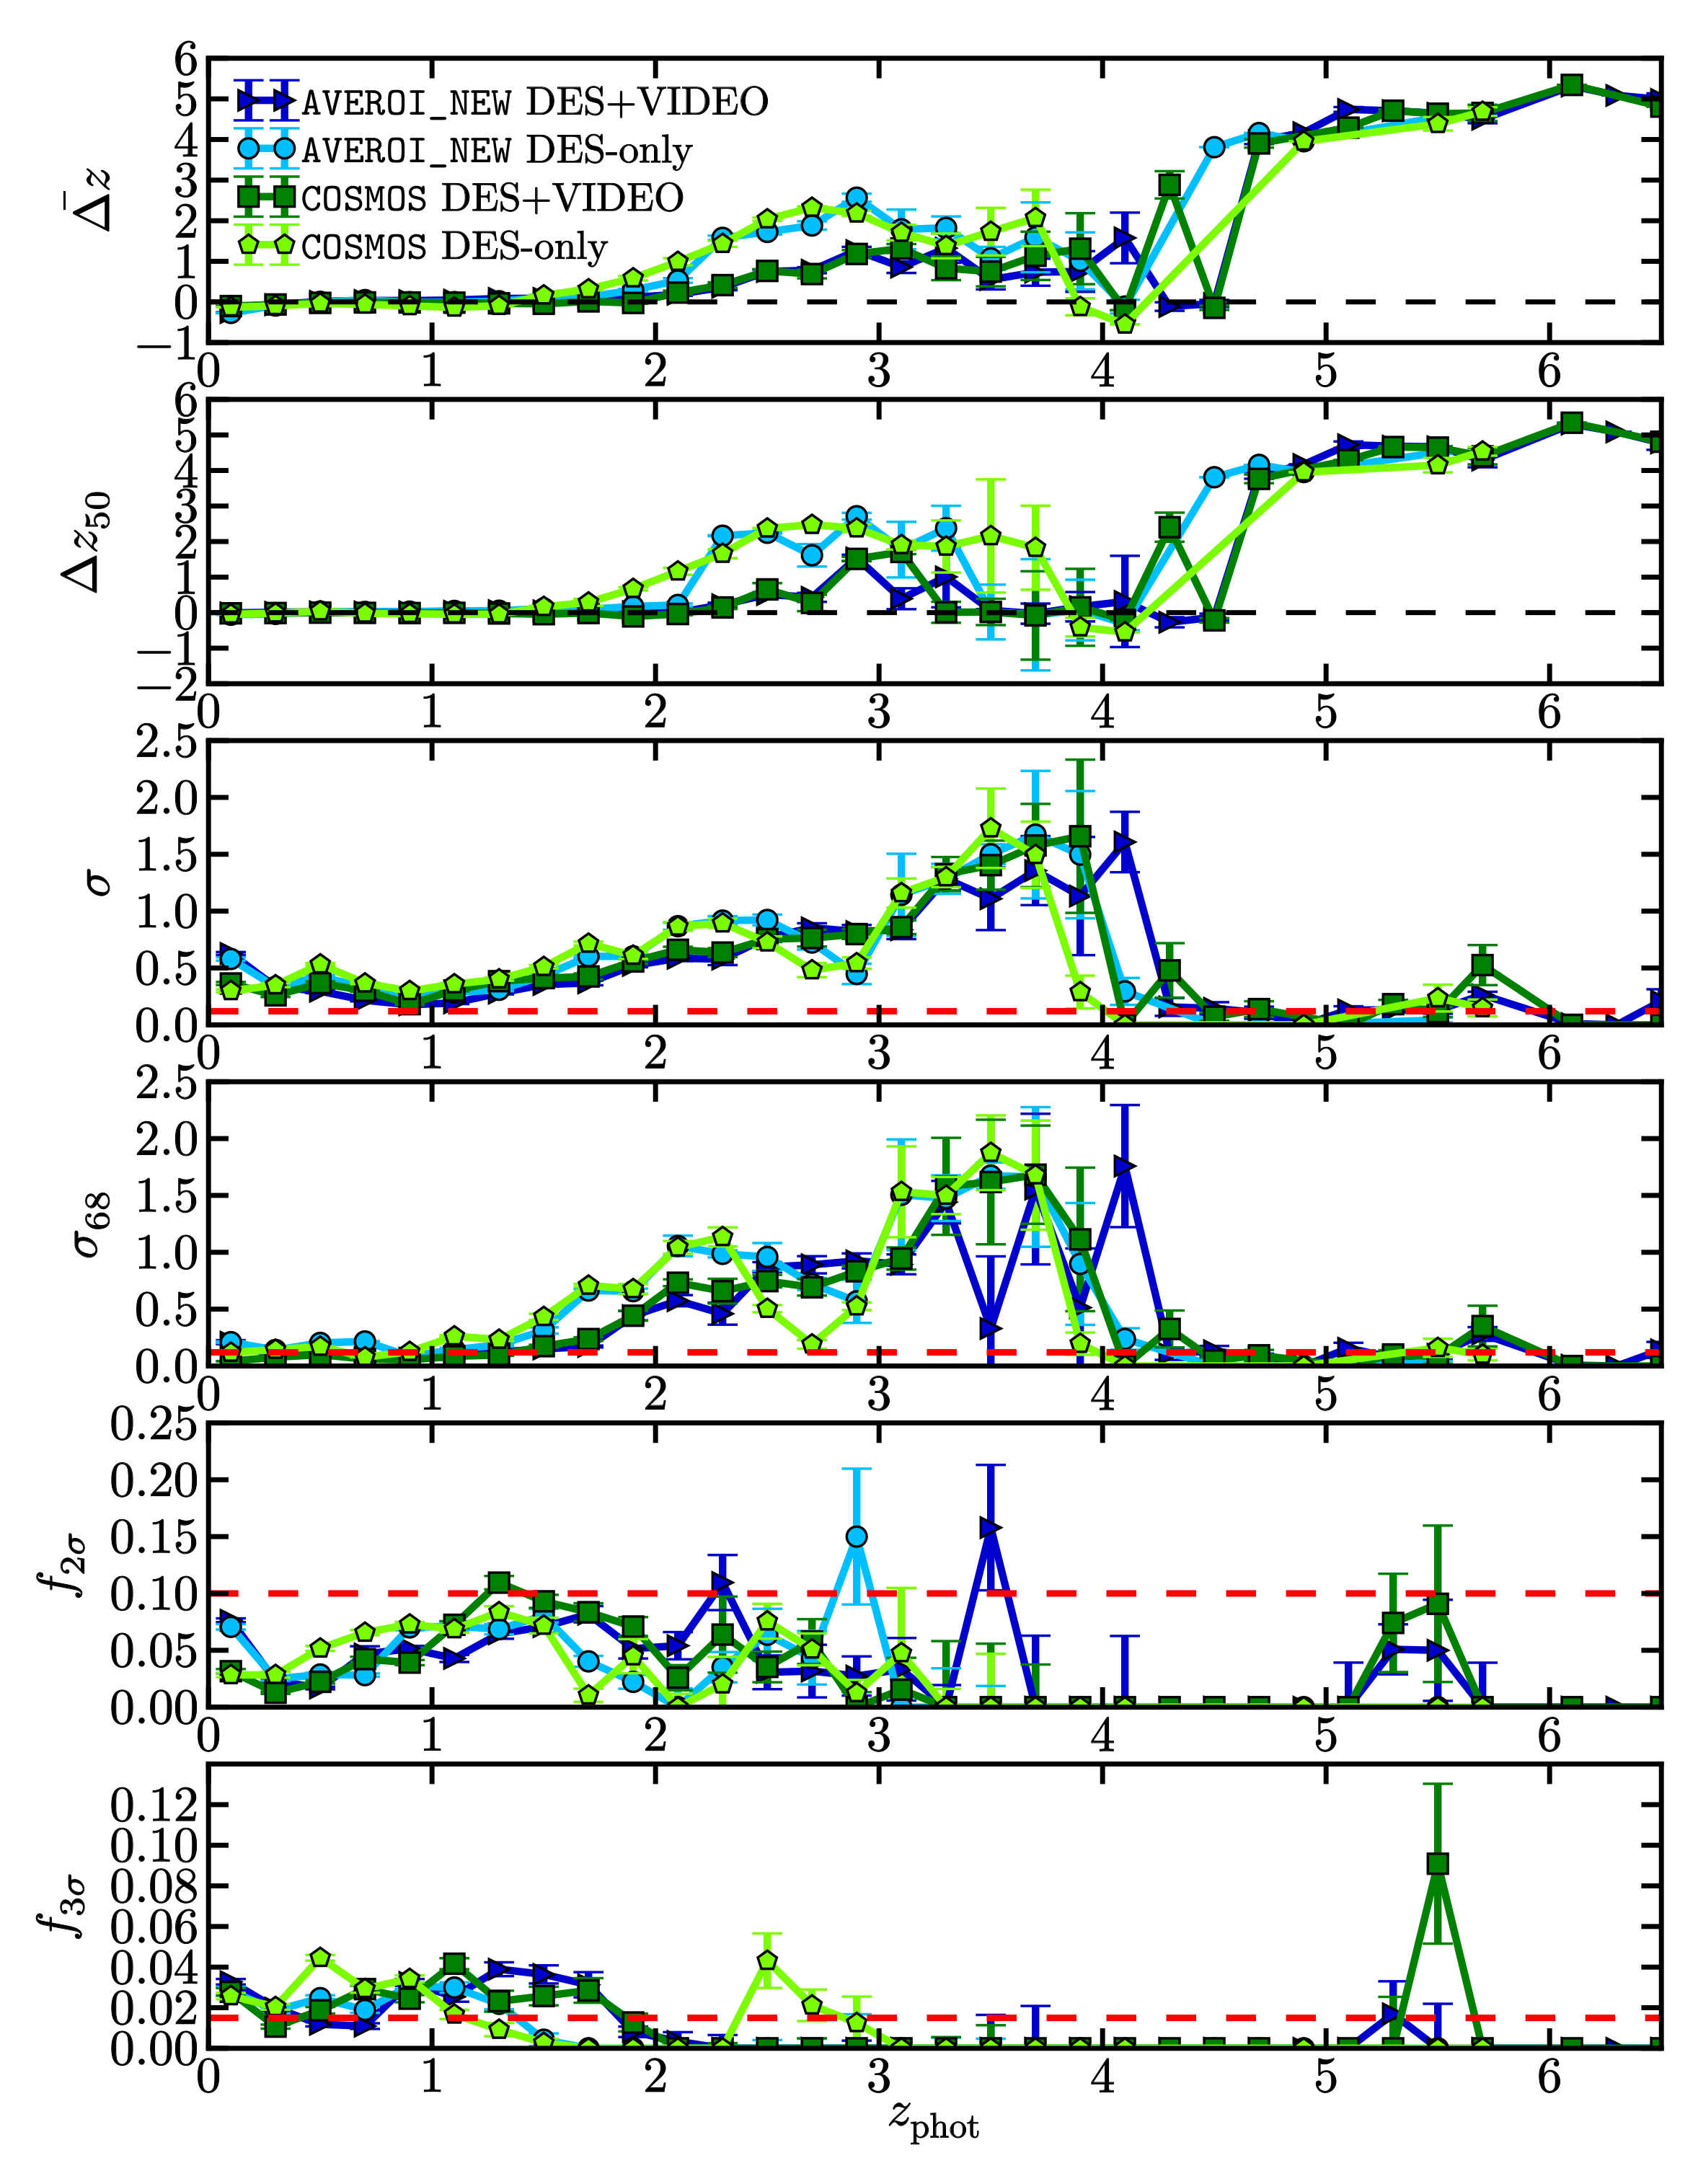
\includegraphics[width=0.95\textwidth]{Chapter3/Figs/basic_des_only_cosmos_cosmos_des_only_photz_long.png}
\caption[Accuracy metrics as a function of photometric redshift between \texorpdfstring{$0<z_{\mathrm{phot}}<6.5$}{}]{The  statistical  metrics  defined  in  Equations \ref{eqn:bias}-\ref{eqn:frac3} as  a  function of photometric redshift,  calculated in redshift bins of $\delta z=  0.2$. Plots have been created via a custom script, adapted by the author based on code written by Matias Carrasco Kind for \cite{2014MNRAS.445.1482S}. Results for the \texttt{AVEROI\_NEW} templates  are  plotted  as  dark  blue  triangles  for  the \texttt{default} (\DESVIDEO) configuration, and light blue circles for the \texttt{des} configuration. Results for the \texttt{COSMOS} templates are shown as dark green squares for the \texttt{default} configuration, and light green pentagons for the \texttt{des} configuration. The red dashed lines in the $\sigma$, $\sigma_{68}$, $f_{2\sigma}$ and $f_{3\sigma}$ plots indicate the DES collaboration requirements on these metrics \citep{2014MNRAS.445.1482S}. When interpreting all six plots, it is important to consider the interplay between the different metrics. Around $z_{\mathrm{phot}} \approx 3$ for instance, the scatter metrics $\sigma$ and $\sigma_{68}$ for the DES-only configurations fall below those of the \DESVIDEO setups. However, a closer look at the $z_{\mathrm{spec}}$ vs $z_{\mathrm{phot}}$ plots (Figures \ref{fig:basic}, \ref{fig:des_only}, \ref{fig:cosmos_basic} and \ref{fig:cosmos_des_only}) shows that this is due to the majority of galaxies in those redshift bins having very low $z_{\mathrm{spec}}<0.5$. This is reflected in the bias metrics, where the DES-only setups show much higher values for $\overbar{\Delta z}$ and $\Delta z_{50}$. Similarly, there is a connection between the value of the outlier fractions $f_{2\sigma}$ and $f_{3\sigma}$ and the value of $\sigma$, where a higher value of $\sigma$ leads to fewer objects being classed as $>2\sigma$ and $>3\sigma$ outliers.}
\label{fig:photoz_long}
\end{figure}

%


\begin{figure}[!htp]
\centering
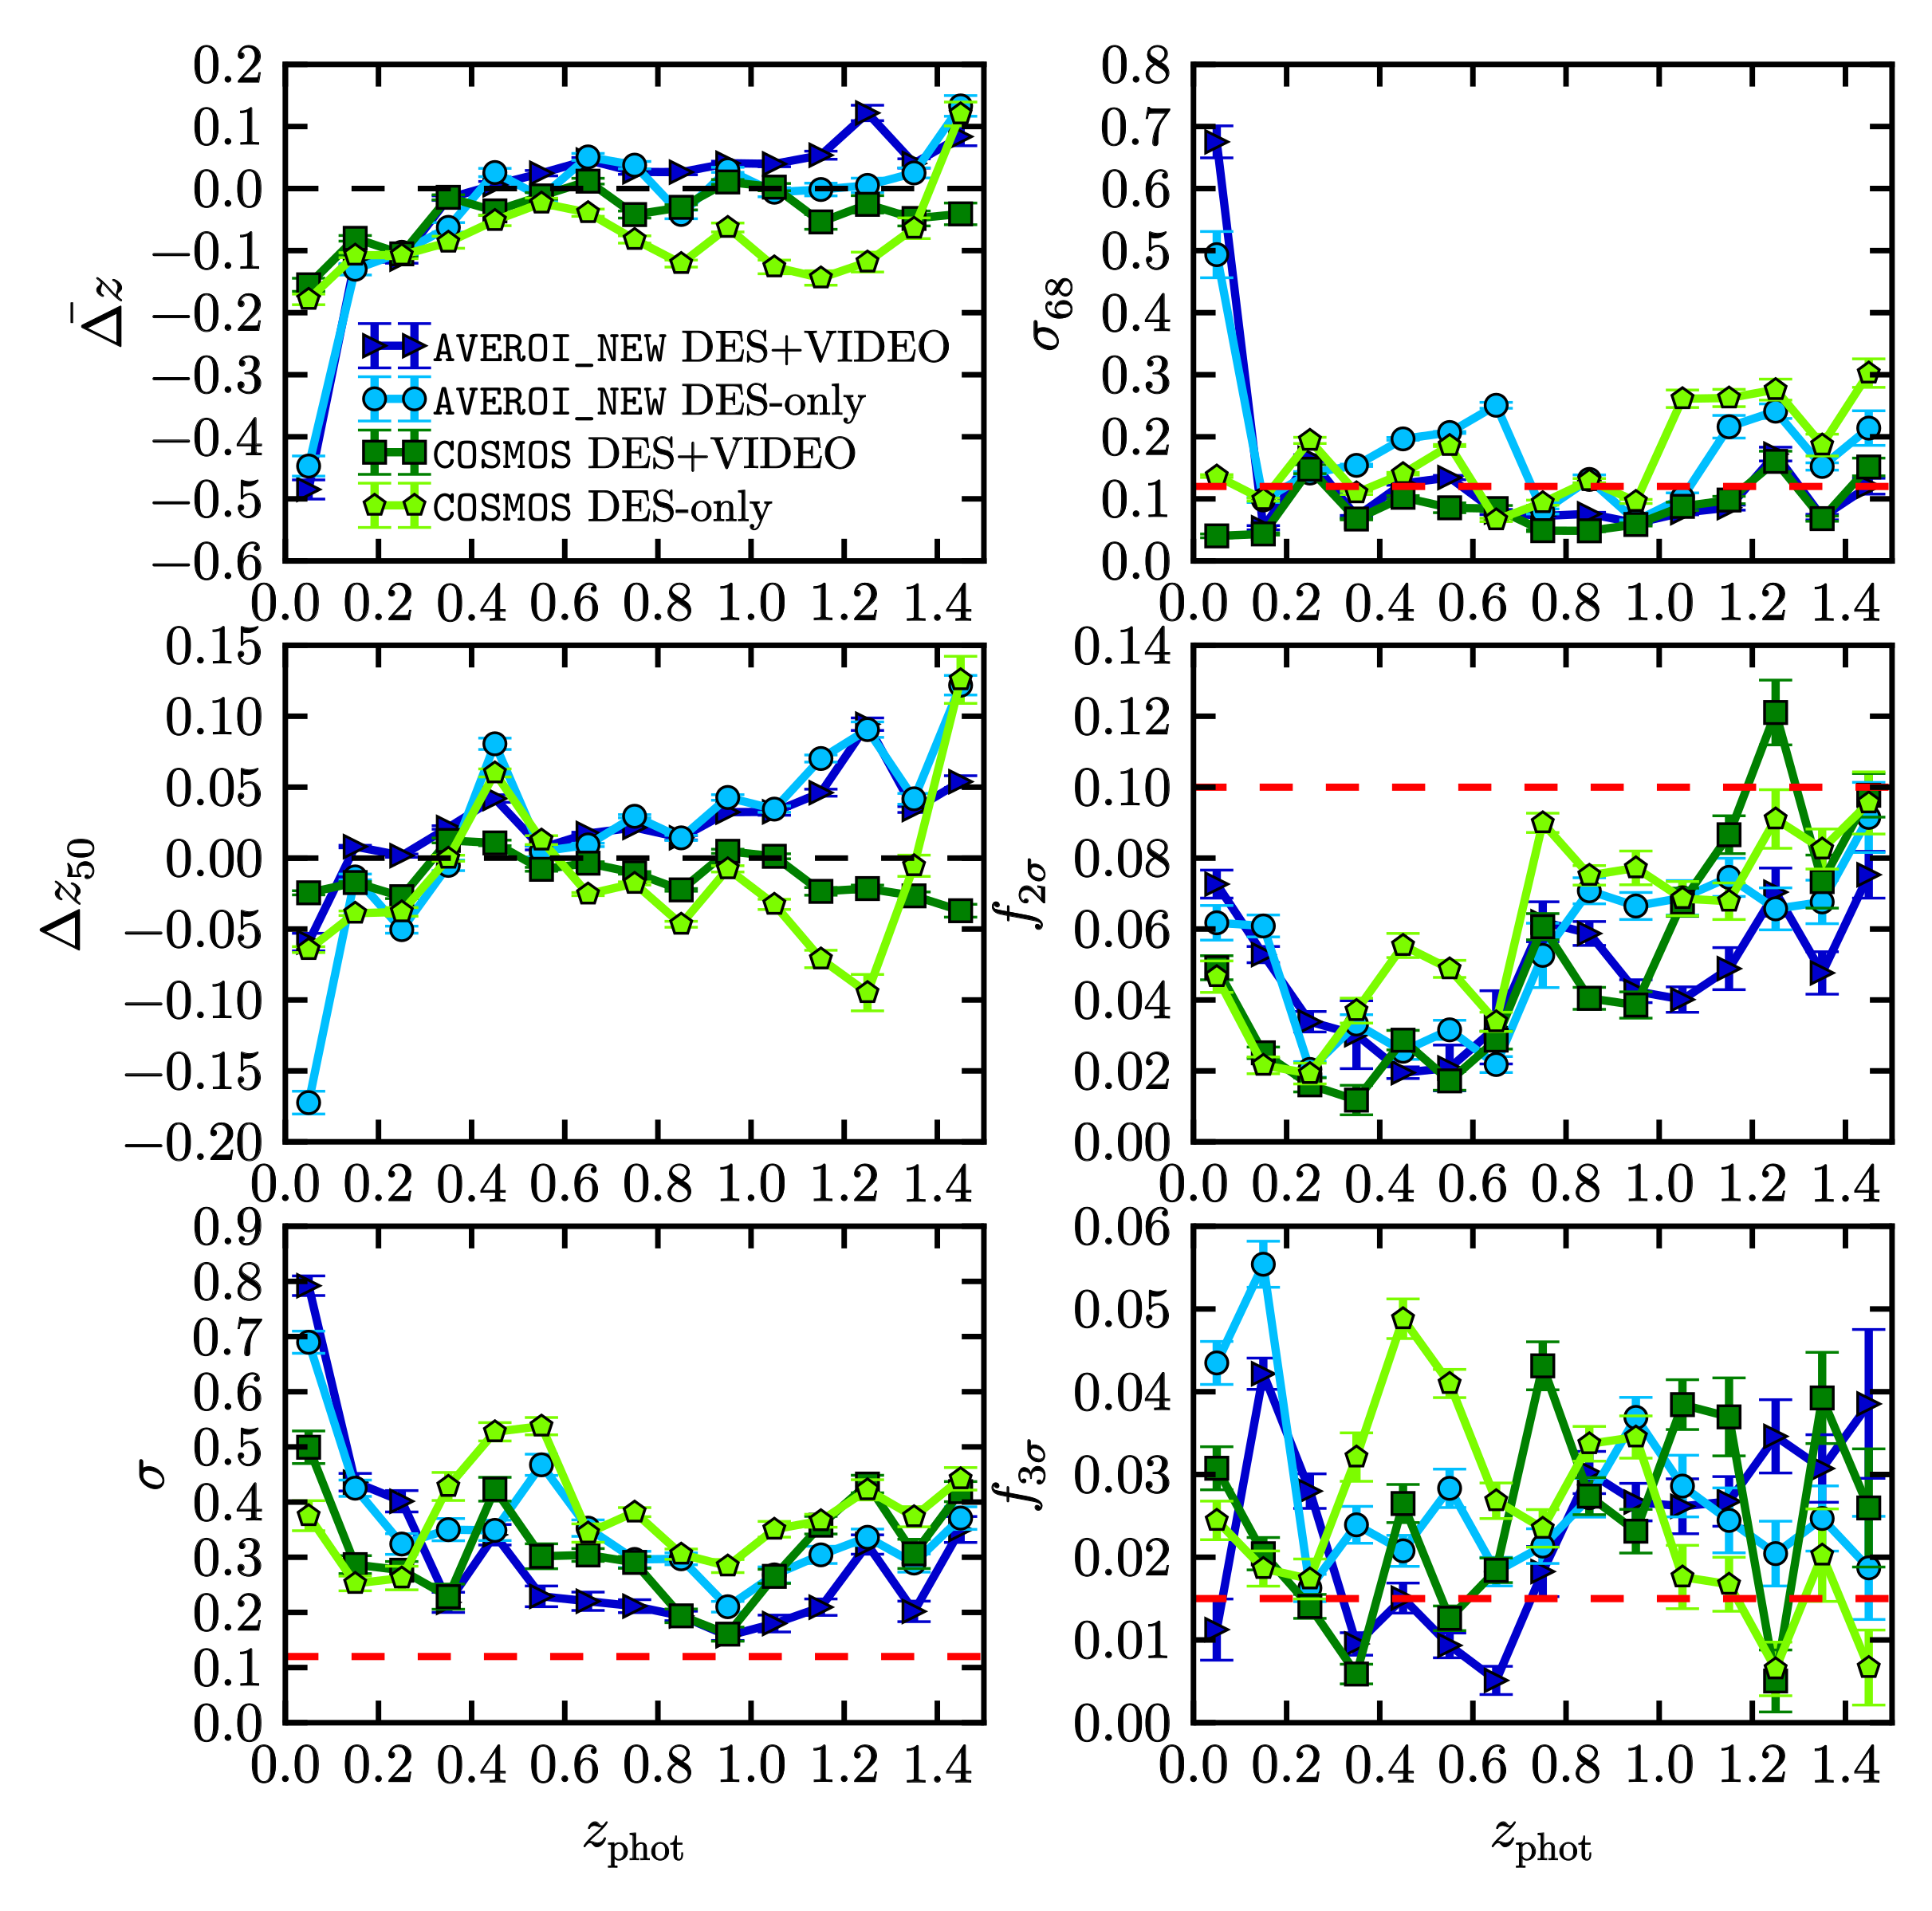
\includegraphics[width=0.95\textwidth]{Chapter3/Figs/basic_des_only_cosmos_cosmos_des_only_photz.png}
\caption[Accuracy metrics as a function of photometric redshift between \texorpdfstring{$0<z_{\mathrm{phot}}<1.5$}{}]{Results from Figure \ref{fig:photoz_long} zoomed in on the low-redshift region $0<z_{\mathrm{phot}}<1.5$, this time using redshift bins of $\delta z=0.1$. In all other aspects, the description is identical to that of Figure \ref{fig:photoz_long}.}
\label{fig:photoz}
\end{figure}

%UNVEIL MORE PRECISELY
%THIS LARGER SCATTER IN DES-ONLY... <2, AS SHOWN IN FIGURE 3.4 WHERE THE SCATTER IS PLOTTED AS A FUNCTION OF Z_PHOT. 
Together, all the plots show more precisely how the near-IR photometry improves the redshifts estimates. The discussion will concentrate on the most notable features. The first of these involves the scatter in the $\Delta z= z_{\mathrm{phot}} - z_{\mathrm{spec}}$ distribution in Figure \ref{fig:photoz_distribution} (\ref{fig:basic} vs \ref{fig:des_only} and \ref{fig:cosmos_basic} vs \ref{fig:cosmos_des_only}). For both template sets, it is clear that the \DESVIDEO distributions are narrower at the core than the DES-only ones. This is the behaviour that causes the observed strong decrease in the $\sigma_{68}$ metric (45.9\% for \texttt{AVEROI\_NEW} and 56.5\% for \texttt{COSMOS}). For the \texttt{COSMOS} plots, the addition of near-IR data leads to considerably less scatter in the tails of the distribution as well. This is reflected in the value of $\sigma$, which is lower for \DESVIDEO by 25.6\% compared to DES-only (at 1.1\% the equivalent improvement is less prominent for the \texttt{AVEROI\_NEW} templates). In general, the larger scatter with DES-only photometry is most notable between $0.3\lesssim z_{\mathrm{phot}} \lesssim 2$. Looking at the scatter as a function of $z_{\mathrm{phot}}$ in Figure \ref{fig:photoz_long}, it becomes apparent that over most of the redshift range the values of $\sigma$ and $\sigma_{68}$ are indeed smaller for the \DESVIDEO configurations than for DES-only. The most prominent exception is the region around $2.7\lesssim z_{\mathrm{phot}} \lesssim3.1$, where  both scatter metrics come out lower without VIDEO data. However, a quick look at the corresponding distributions in Figure \ref{fig:photoz_distribution} demonstrates this reduced scatter does not correspond to better photo-z performance. Instead it is simply a result of a consistently stronger bias; above $z_{\mathrm{phot}}\gtrsim 2.7$ almost all objects in the DES-only dataset lie at $z_{\mathrm{spec}}\sim0$, leading to low scatter centred around a false result. The second exception is the region around $z_{\mathrm{phot}} \sim 0$ for the \texttt{AVEROI\_NEW} templates. In this region, most notable in Figure \ref{fig:photoz}, the \DESVIDEO configuration shows slightly higher scatter metrics. Figure \ref{fig:basic} demonstrates that this effect originates from the large number of objects at any $z_{\mathrm{spec}}$ that are assigned $z_{\mathrm{phot}}\sim0$, which most likely occurred as a result of template incompleteness. This problem is localised to $z_{\mathrm{phot}}\sim0$. Apart from the two exceptions stated above, the inclusion of near-IR data generally leads to lower scatter at almost all redshifts. This is an important result for  photometric redshift studies, as low scatter is often desirable for cosmology \citep{2014MNRAS.445.1482S, 2008MNRAS.386.1219B, 2011MNRAS.414..329C, 2012MNRAS.420.3240N}. \par

%I GOT UP TO HERE LOOK AT THE LAST FEW SENTENCES

%NEAR-IR CAN REDUCE THE SCATTER CONSIDERABLY

%GET RID OF THE FOOTNOTE/LY BREAK ONLY ENTERS BETWEEN Z1 AND Z2

The second main improvement that comes with the addition of near-infrared data concerns the reduction of outliers. Photometric redshifts heavily rely on strong spectral features, such as the Lyman and \SI{4000}{\angstrom} breaks. With only $griz$ DES data, the photo-zs enter the so-called `redshift desert' \citep{2001AJ....122.2205R,2006A&A...457..841I} at $z\gtrsim1.5$, as the \SI{4000}{\angstrom} break shifts out of the $z$-band. Because the Lyman break only enters the $g$-band between\footnote{Depending on the amount of absorption in the Lyman-$\alpha$ forest, the rest-frame Lyman break lies between \SI{912}{\angstrom} (the Lyman limit) and \SI{1216}{\angstrom} (Lyman-$\alpha$), see e.g. Section \ref{subsubsection:lyman_break} and \cite{1995ApJ...441...18M}.} $z=2.3$ and $z=3.4$, without near-IR data there are no strong continuum features available to constrain the redshift of objects between $1.5\lesssim z \lesssim 3$. As a result, the DES-only results in Figures \ref{fig:des_only} and \ref{fig:cosmos_des_only} show a large number of outliers between $ 2 \lesssim z_{\mathrm{phot}} \lesssim 3$, mainly with $z_{\mathrm{spec}}\lesssim0.5$. Many of these are galaxies without a strong \SI{4000}{\angstrom} break, for which the code erroneously assumes that the absence of a such a feature must mean the Lyman break lies unobserved at $ 2 \lesssim z_{\mathrm{phot}} \lesssim 3$. The addition of near-infrared data removes this degeneracy, as the absence of a \SI{4000}{\angstrom} break can now be confirmed in the VIDEO $YJH$-bands. The effectiveness of near-infrared data at overcoming problems to do with the redshift desert is also illustrated by Figure \ref{fig:photoz_long}. From $z\gtrsim 1.5$ onwards, the bias metrics $\Delta z$ and $\Delta z_{50}$ start to deviate more strongly from zero for the DES-only plots (compared to their \DESVIDEO counterparts). Similarly, the scatter as indicated by $\sigma$ and $\sigma_{68}$ also increases sharply. The importance of the VIDEO data is observed the most in the value of $\Delta z_{50}$, which stays close to zero for most of the $1.5<z<3$ redshift range when near-IR data is included. \par

%DON'T USE STRONGLY SO MUCH 

Figure \ref{fig:photoz} focuses on the value of near-infrared data for the local ($z<1.5$) end of the spectroscopic subsample. This redshift range contains the bulk of the available spectra (see Figure \ref{fig:spectra}), and is of particular interest for cosmological applications of photo-zs. The plots demonstrate that in most redshift bins, the values for the \DESVIDEO metrics are lower than for DES-only. It is also interesting to consider the red dashed lines for $\sigma$, $\sigma_{68}$, $f_{2\sigma}$, and $f_{3\sigma}$, which show the DES collaboration requirements on these metrics \citep{2014MNRAS.445.1482S}. The importance of near-infrared data is especially apparent for $\sigma_{68}$, where the values in most bins only lie below the specified requirement when VIDEO data is added. \par

%ALL (photo-z) RESULTS??? ALSO RESULTS OR CONCLUSIONS
The discussion on near-IR data will now conclude with some final remarks. As mentioned at the beginning of this chapter, the reader must bear in mind that the configurations in this thesis have been designed primarily with high-redshift performance in mind. Regarding the conclusions for general photo-z research, this affects several aspects. Most importantly, the choice of code was informed by the fact that template fitting codes are more suitable in this regime. Results are therefore presented with the caveat that they are not explicitly proven to hold for empirical methods. Naturally, a related limitation is that the research in this chapter has only been performed using \texttt{LePHARE}. Extending this work to other codes is therefore presented as a topic for further study (although at low redshifts several comparative studies already exist, see e.g.  \citealt{2010A&A...523A..31H,2011MNRAS.417.1891A,2014MNRAS.445.1482S}). Furthermore, the setups used in the near-IR analysis all include emission lines, even though Section \ref{subsubsection:discussion_emlines} indicated that emission lines do not conclusively improve the non-high-redshift results for the \texttt{AVEROI\_NEW} templates. However, the small worsening in some metrics between the \texttt{default} and \texttt{no\_emlines} setups is considerably less than the improvement with VIDEO data, so it is expected that near-IR data will still be beneficial if emission lines are omitted. Lastly, the third possible high-redshift bias lies in the use of fixed aperture magnitudes, which Section \ref{subsubsection:auto_magnitudes} found to perform slightly worse for the \texttt{AVEROI\_NEW} templates in some metrics. However, a comparison between the \texttt{auto} and \texttt{des\_auto} metrics in Table \ref{table:photoz_test} confirms that using near-IR data leads to considerable improvements with auto photometry as well.\par

\subsubsection{Template sets revisited}\label{subsubsection:templates_revisited}
Let us now return to the question of template set choice raised in Section \ref{subsubsection:template_sets}. The preceding analyses of the \texttt{AVEROI\_NEW} setups have concluded that for those SEDs the \texttt{more\_ext} configuration is the most suitable for this thesis (i.e. when judged primarily by the expected high-redshift performance). For the \texttt{COSMOS} templates, the \texttt{default} configuration emerged as the best-performing set of options, at high redshifts as well as over the full (low-z dominated) redshift range. \par

For the sake of versatility, it was decided to run both these best-performing setups on the full \DESVIDEO catalogue. Anyone who wishes to use the catalogue can then choose which template set is most appropriate for their particular science goals. For instance, the high-redshift search later in this thesis makes use of the \texttt{AVEROI\_NEW} templates, for reasons that will be explained in Section \ref{subsection:template_choice}. Lower redshift applications, on the other hand, may benefit from using the \texttt{COSMOS} photo-zs instead, as Section \ref{subsubsection:template_sets} demonstrated that these templates performed better in almost all non-high-redshift metrics.\par




\section{Full \DESVIDEO catalogue}\label{section:full_catalogue}
After it was decided to use the \texttt{AVEROI\_NEW more\_ext} and \texttt{COSMOS default} setups as the final configurations, photometric redshifts were generated for all \num{2 443 576} sources in the full \DESVIDEO catalogue. As before, these redshifts have been calculated by running \texttt{LePHARE} per VIDEO tile, calibrating the adaptive offsets in the same way as for the spectroscopic subsample in Section \ref{subsection:photoz_computation_method}. The results were then added to the \DESVIDEO catalogue from Chapter \ref{chapter:catalogue}. \par

Before any meaningful scientific inferences can be made from the photo-zs, it is necessary to eliminate sources that are stars, as these of course have nonsensical redshift estimates. The current section will therefore firstly address finding a suitable star-galaxy separation strategy. Along the way, the analysis will also discuss the extent to which the VIDEO data helps to distinguish between galaxies and stellar sources. The final part of this section will then present the photometric redshifts for all galaxies in the \DESVIDEO dataset, obtained after filtering out stars via the established method. \par




\subsection{Star-galaxy separation}\label{subsection:star_galaxy}
\subsubsection{Background}\label{subsubsection:star_galaxy_background}
Finding a reliable way of filtering out stars is crucial for ensuring that the \DESVIDEO catalogue is suitable for future studies of galaxy evolution and cosmology. Such a star-galaxy separation strategy is also necessary for the $z\gtrsim5$ galaxy search later in this thesis, as stars are known contaminants among high-redshift samples. Furthermore, the study of how to differentiate between galaxies and stellar sources is of general interest to the scientific community, so it is important to investigate what insights the \DESVIDEO catalogue can offer. \par


Common star-galaxy separation methods in the literature often employ morphological strategies. In recent years, use of the \texttt{spread\_model} classifier has become popular \citep{2012ApJ...757...83D, 2015MNRAS.450..666S, 2015MNRAS.446.2523B}. This parameter is computed by \texttt{SExtractor} as a discriminant between the best-fitting PSF model and an extended disk model. Other morphology-based options in the literature have included the use of neural networks, such as the \texttt{CLASS\_STAR} parameter in \texttt{SExtractor} \citep{2003MNRAS.344..337T,2015A&A...582A..62D,2018MNRAS.481.5451S} or custom machine learning methods \citep{2015MNRAS.450..666S,2018MNRAS.481.5451S}. However, at $z\sim 6$, galaxies are frequently small in size \citep{2012ApJ...744...83O,2016MNRAS.457..440C}, which means that they are not reliably resolved in ground-based surveys with similar seeing to \DESVIDEO. While some objects in ground-based high-redshift samples show resolved light-profiles \citep{2012MNRAS.426.2772B}, overall roughly half the candidates are unresolved \citep{2013AJ....145....4W, 2014MNRAS.440.2810B}, and the apparent sizes are generally dominated by the seeing \citep{2015MNRAS.452.1817B}. Subsequently, morphological criteria would likely not be effective in distinguishing between stars and galaxies at high redshifts. \par

Alternative methods based on colour information are therefore more appropriate for the purpose of this thesis. Some authors have performed star-galaxy separation via simple colour-colour cuts based on optical and near-IR photometry (e.g. \citealt{2010MNRAS.404...86B, 2013MNRAS.428.1281J}). Others have employed an SED-based approach using the full range of photometry from all available filters, by fitting star SEDs and rejecting objects from a high-$z$ sample if they show good stellar fits (e.g. \citealt{2014MNRAS.440.2810B,2015MNRAS.452.1817B}). \par

\subsubsection{A \texorpdfstring{$\chi^2_{\nu}$}{TEXT}-based method}\label{subsubsection:chi_method}
This thesis has opted to investigate an SED-based approach. \texttt{LePHARE}'s inbuilt capacity to fit stellar SEDs makes such a strategy straightforward to implement, since the code assigns every object a best-fit galaxy, QSO, and stellar template with corresponding $\chi^2$ in the output files. This $\chi^2$ can  be converted\footnote{This is necessary in order to enable meaningful comparisons between objects with varying numbers of observed filters.} straightforwardly to a reduced $\chi_{\nu}^2$ via Equation \ref{eqn:red_chi_squared}.  Star-galaxy separation can then be performed by requiring that any object designated as a galaxy must have a lower galaxy reduced $\chi^2_{\nu,\mathrm{gal}}$ compared to its star fit $\chi^2_{\nu,\mathrm{star}}$: 

\begin{equation}
\chi^2_{\nu,\mathrm{gal}} - \chi^2_{\nu,\mathrm{star}} < \Delta \chi^2_{\nu}. \label{eqn:star_galaxy}
\end{equation}

\noindent Here, $\Delta \chi^2_{\nu}$ is a threshold that can be adjusted according to the desired strength of the separation cut. A value of $\Delta \chi^2_{\nu} = 0$ dictates that any object designated as a galaxy must simply show a better galaxy fit than a star fit. Negative values of $\Delta \chi^2_{\nu}$ produce a stricter selection, with more negative values generating increasingly conservative cuts. The star-galaxy separation method in the rest of the current chapter employs a threshold of $\Delta \chi^2_{\nu}=0$. For the selection of a high-redshift sample in Chapter \ref{chapter:high_redshift_candidates}, a lower value of $\Delta \chi^2_{\nu}=-1.5$ is imposed. \par


\subsubsection{Method validation}\label{subsubsection:star_galaxy_validation}
In order to validate the above method, it has been trialled on the \DESVIDEO \texttt{LePHARE} output, using the fits from both the \texttt{AVEROI\_NEW} and \texttt{COSMOS} SEDs. The results were then compared to a truth catalogue based on spectroscopic and space-based observations, provided by Nacho Sevilla-Noarbe on behalf of the DES collaboration\footnote{For the sake of producing reproducible research, it should be mentioned that this catalogue was titled \texttt{round5\_101\_testing\_master.fits}.}. A similar truth catalogue is described in \cite{2018MNRAS.481.5451S}. The dataset contains a total of \num{226 611} sources with classifications. Of these, \num{73 551} matched to the (non-duplicate) \DESVIDEO catalogue within a \SI{1}{\arcsec} radius. Sources flagged as galaxies (\texttt{TRUE\_CLASS} = 1) account for \num{64 326} of this total, and stars (\texttt{TRUE\_CLASS} = 0) for 982. The 9225 remaining objects are either classified as QSOs or uncertain. Of the 982 objects listed as stars, 132 also occur in the DES galaxy spectroscopic redshift catalogue (introduced in Section \ref{subsection:spectra}); these sources were removed from the list of stars in order to achieve maximum confidence that the truth sample indeed consists solely of stars. Finally, to reduce the chance of any biases through faulty photometry, any sources that contain non-zero values for the \texttt{FLAGS\_WEIGHT} parameters were also removed (the process and justification for this is the same as in Section \ref{section:photoz_computation}). The final truth sample then consists of 847 stars and \num{62 951} galaxies, leading to a total truth catalogue containing \num{63 798} sources.\par

Using the \texttt{AVEROI\_NEW} SED fits, the star-galaxy separation method proposed in Section \ref{subsubsection:chi_method} (applying Equation \ref{eqn:star_galaxy} with a loose cut of $\Delta \chi^2_{\nu} =0$ to fits based on \DESVIDEO photometry) classifies 2895 of the total \num{63 798} sources as stars and \num{60 903} as galaxies. Out of the 847 real stellar sources, 834 (98\%) are indeed retrieved as stars. Only 15 (1.8\%) actual stars are falsely designated as galaxies. This implies that the \textit{stellar contamination} --- defined as the ratio between the number of stars misidentified as galaxies to the total number of sources classified as galaxies \citep{2015MNRAS.450..666S} --- equals\footnote{It is stressed that because the ratio of stars to galaxies in the truth catalogue is not representative of the true numbers in the \DESVIDEO fields, the stellar contamination does not give an accurate view of the absolute expected fraction of misclassified stars. However, the values are nevertheless valuable for a comparison between different photo-z configurations; because all the verification tests use the same truth catalogue, they give an indication of which setup is likely to contain the most contamination from stars.} 0.025\%. Moreover, 60 888  true galaxies (97\%) are confirmed as galaxies. This percentage  --- i.e. the ratio of the number of true well-classified galaxies to the number of total true galaxies --- is sometimes referred to as the galaxy \textit{completeness} \citep{2015MNRAS.450..666S}. Finally, 2063 (3.3\%) real galaxies are wrongly classified as stars. When repeating the above analysis with the \texttt{COSMOS} fits, the proposed separation strategy finds 2275 stars and \num{61 523} galaxies. It correctly identifies a total of 828 (98\%) true stars and misjudges 19 (2.2\%) as galaxies, implying a stellar contamination rate of 0.031\%. In the same vein, 61 504 (98\% galaxy completeness) true galaxies are correctly classified and 1447 (2.3\%) are wrongly classified as stars. Figures \ref{fig:star_galaxy_des_video}  and \ref{fig:star_galaxy_cosmos_des_video} further illustrate the separation results, showing the full $\chi^2_{\nu,\mathrm{gal}} - \chi^2_{\nu,\mathrm{star}}$ distributions of the true stars and galaxies for the two template sets. When comparing all the results for the two configurations, it is apparent that the \texttt{COSMOS} SEDs perform slightly better in terms of galaxy completeness. On the flip side, however, they also show higher stellar contamination. A likely explanation for these observations is the lower galaxy $\chi_{\nu}^2$ found among the \texttt{COSMOS} fits, leading to lower values of $\chi^2_{\nu,\mathrm{gal}} - \chi^2_{\nu,\mathrm{star}}$ (because the two configurations use the same set of stellar templates, $\chi^2_{\nu,\mathrm{star}}$ remains almost\footnote{The two configurations produce different adaptive offsets, so the $\chi^2_{\nu,\mathrm{star}}$ may also vary ever so slightly.} entirely the same).  Therefore, more objects satisfy the $\chi^2_{\nu,\mathrm{gal}} - \chi^2_{\nu,\mathrm{star}} < 0 $ criterion for galaxy classification. As a result, more true galaxies are assigned galaxy status with the \texttt{COSMOS} SEDs, leading to higher galaxy completeness, but more true stars are classified as galaxies as well, increasing stellar contamination. \par


\begin{figure}
\centering
\subfloat[\label{fig:star_galaxy_des_video}]{
	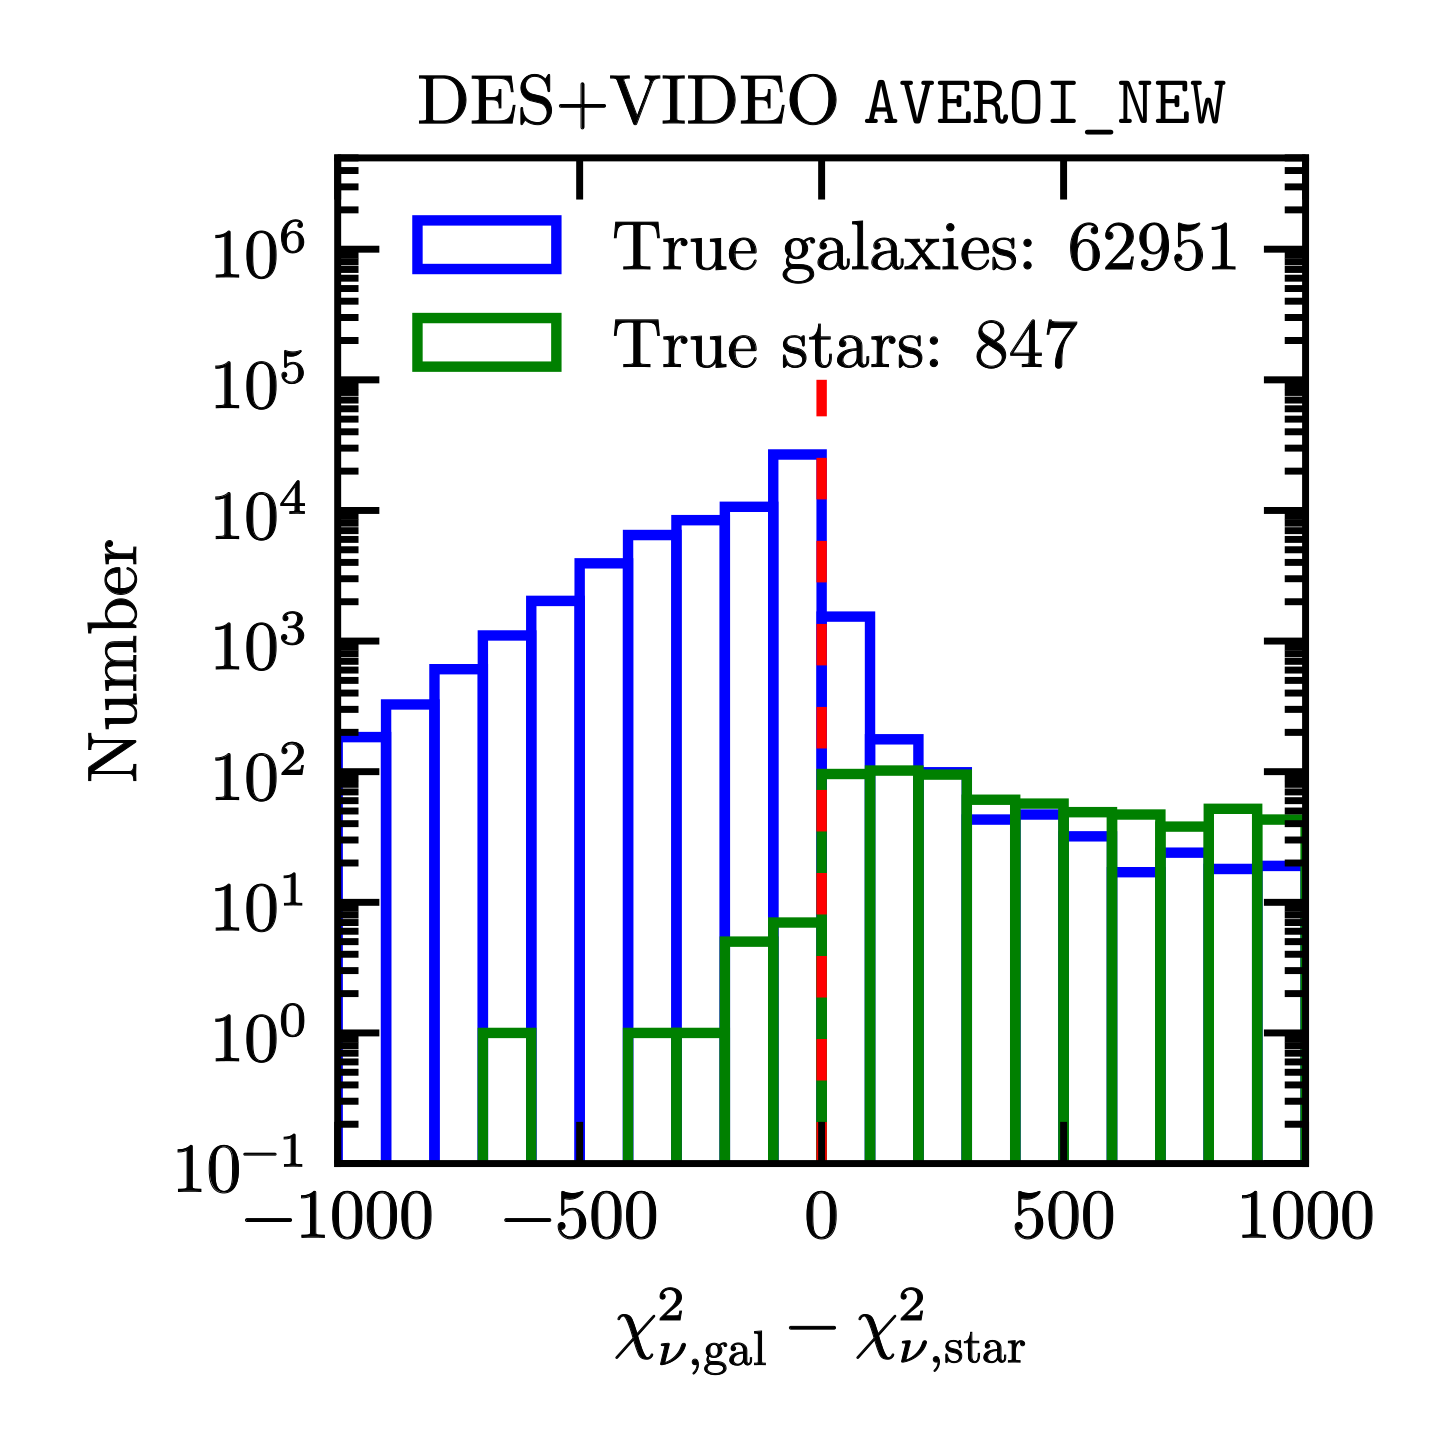
\includegraphics[clip, width=0.50\textwidth]{star_galaxy_des_video_reduced.png}}
\subfloat[\label{fig:star_galaxy_des_only}]{
	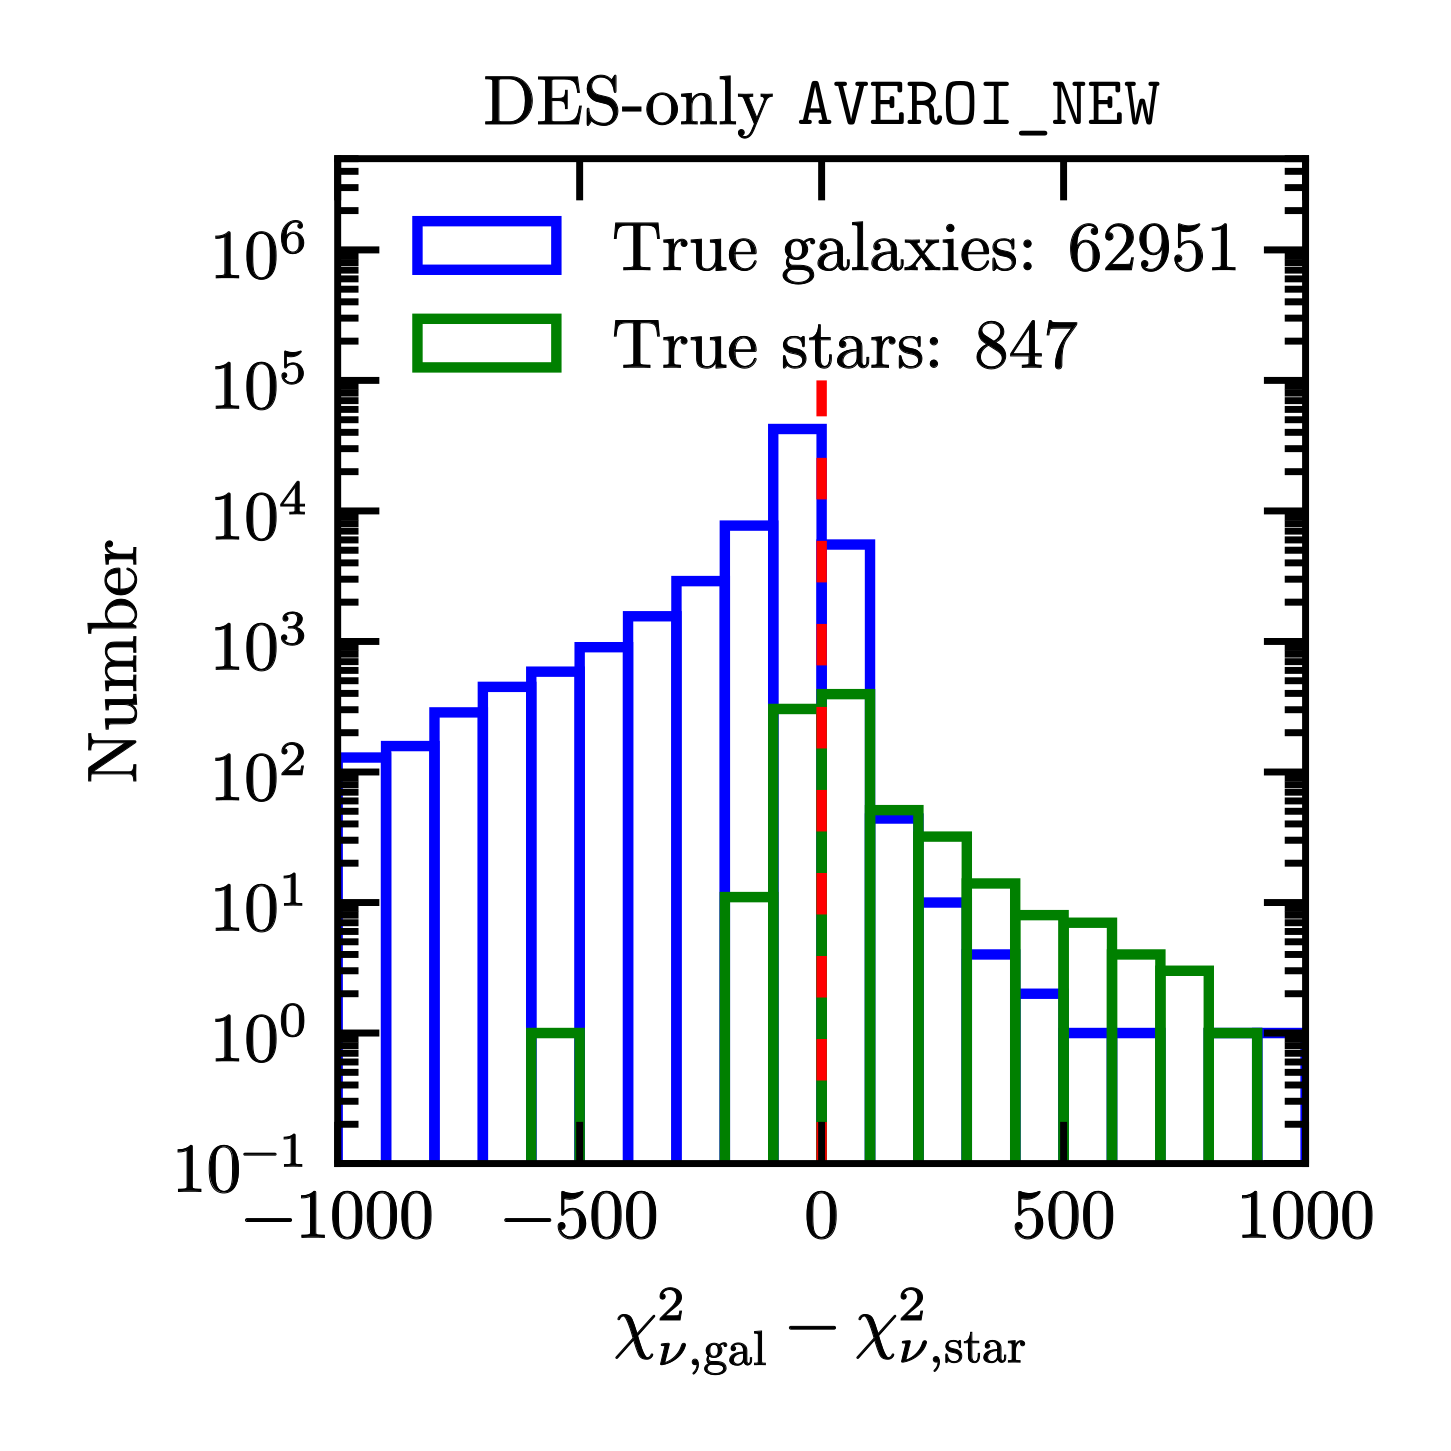
\includegraphics[clip, width=0.50\textwidth]{star_galaxy_des_only_reduced.png}}

\subfloat[\label{fig:star_galaxy_cosmos_des_video}]{
	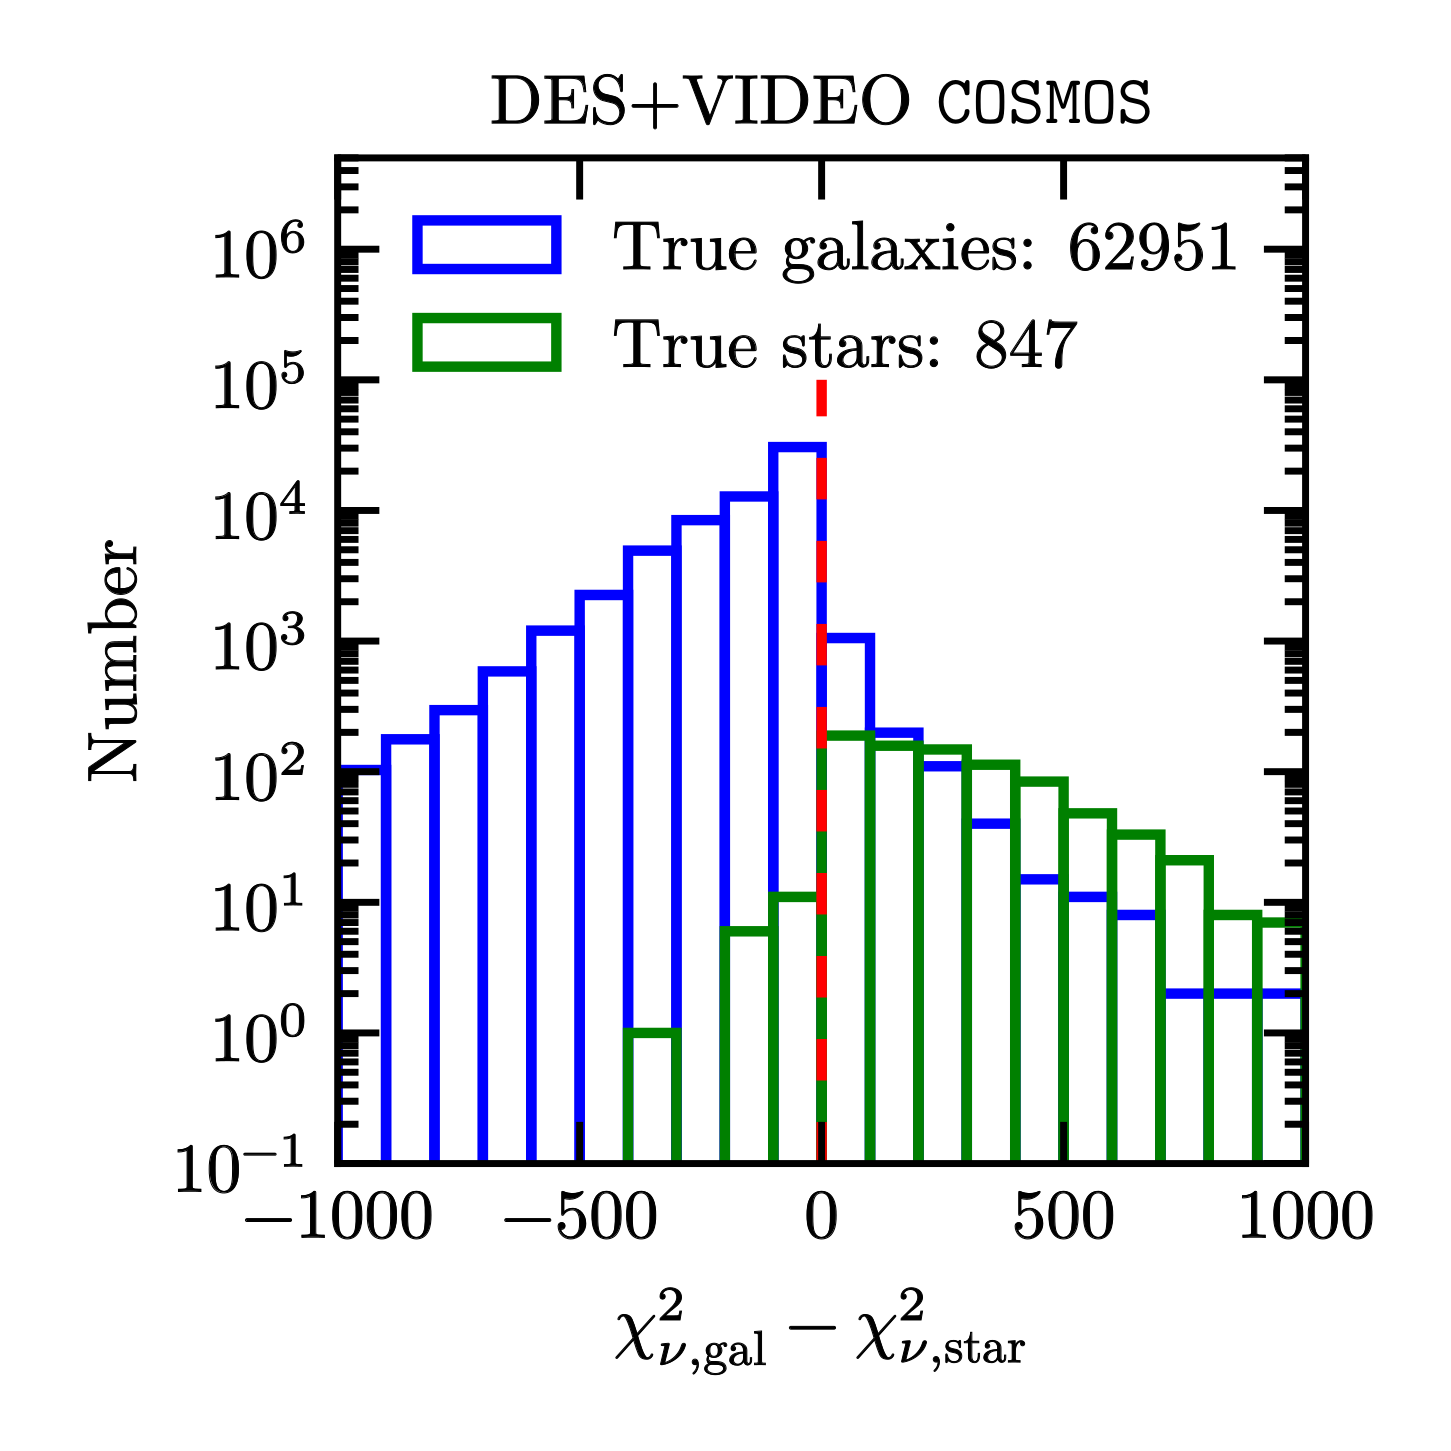
\includegraphics[clip, width=0.50\textwidth]{star_galaxy_cosmos_des_video_reduced.png}}
\subfloat[\label{fig:star_galaxy_cosmos_des_only}]{
	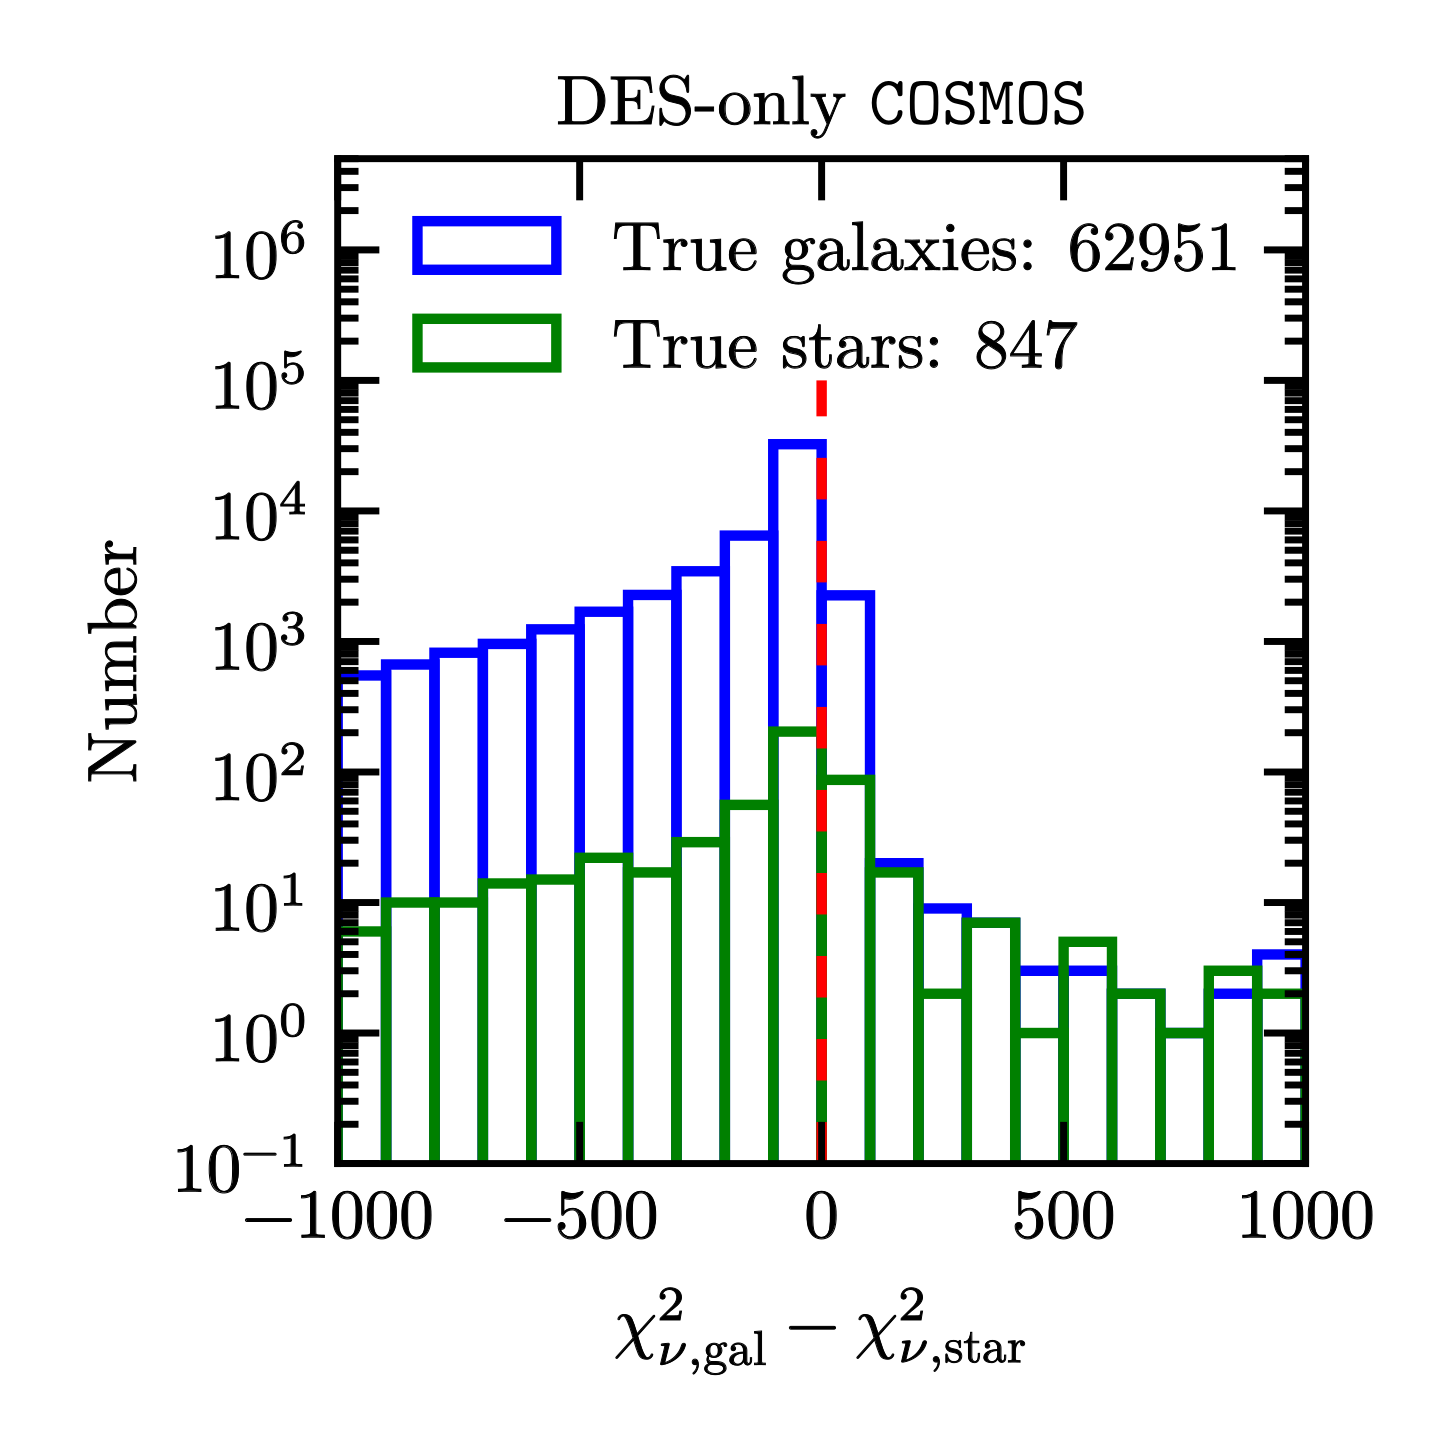
\includegraphics[clip, width=0.50\textwidth]{star_galaxy_cosmos_des_only_reduced.png}}
\caption[Star-galaxy separation verification]{The star-galaxy separation strategy proposed in this thesis, which is based on reduced $\chi^2_{\nu}$ values for the best-fit star and galaxy templates computed by \texttt{LePHARE}. Objects consist of all non-duplicate sources in the \DESVIDEO footprint matched to a truth catalogue (see the text), comprising a total of 847 true stars (green bars) and \num{62 951} true galaxies (blue bars). The red line shows the separation threshold $\chi^2_{\nu,\mathrm{gal}}- \chi^2_{\nu,\mathrm{star}} = 0$. The technique in this chapter classifies objects to the left of this line as galaxies, and objects to the right as stars. Figures  \textbf{(a)} and \textbf{(c}) show the results for template fitting using both DES and VIDEO data for the \texttt{AVEROI\_NEW} and \texttt{COSMOS} templates respectively. Figures  \textbf{(b)} and \textbf{(d}) show the results using DES data only.  Further discussion is provided in the text.}
\label{fig:star_galaxy}
\end{figure}


Regardless, it can be concluded that for both template sets the suggested star-galaxy separation strategy  is highly effective, with a failure rate of around 2--3\% for both stars and galaxies. Despite this excellent prognosis though, it must be remarked that most of the objects in the validation truth catalogue are relatively bright. Such sources are generally expected to have the highest quality photometry, and it is possible that the current method is less accurate at the faint magnitudes that are typical in high-redshift research, where photometric uncertainties are higher. However, this issue  affects any star-galaxy separation technique based on broadband imaging alone, including the morphology-based strategies mentioned in Section \ref{subsubsection:star_galaxy_background}. All things considered, the good performance of the proposed $\chi_{\nu}$-based technique on the validation truth catalogue instills confidence that the technique will be competitive at high redshifts as well. \par


\subsubsection{The effect of near-IR data}\label{subsubsection:method_validation_near_IR}
%THE ABOVE ANALYSIS WAS REPEATED
It is interesting to investigate to what extent the star-galaxy separation is helped by the inclusion of near-IR data. To answer this question, \texttt{LePHARE} was run on the truth catalogue sources using only DES $griz$ photometry (via the \texttt{des} setups introduced in Section \ref{subsection:alternative_setups}), and the separation procedure from the previous section was repeated.  This time, classification based on the \texttt{AVEROI\_NEW} templates selects 6128 (supposed) stars and \num{57 670} galaxies. The selection correctly identifies only 531 (64\%) true stars, and falsely classifies 316 (36\%) as galaxies, leading to a stellar contamination rate of 0.55\%. Regarding true galaxies, \num{57354} sources are correctly retrieved, implying a galaxy completeness of 91\%. The remaining 5597 (8.9\%) true galaxies are misclassified as stars. For the \texttt{COSMOS} templates, which find 2515 stars and \num{61 283} galaxies, most numbers are even less favourable; only 190 (22\%) of the actual stars are correctly classified, and a majority of 657  (78\%) true stars are wrongly identified as galaxies, leading to a substantially worse stellar contamination of 1.1\%. The galaxy completeness is slightly better than for the \texttt{AVEROI\_NEW} templates, with \num{60 626} (96\%) of the true galaxies classified properly. The other 2325 (3.6\%) true galaxies are wrongly judged to be stars. Figures \ref{fig:star_galaxy_des_only} and \ref{fig:star_galaxy_cosmos_des_only} provide a more detailed view of the performance, plotting the $\chi^2_{\nu,\mathrm{gal}} - \chi^2_{\nu,\mathrm{star}}$ distributions for both template sets. \par



A direct comparison between these DES-only results and the earlier \DESVIDEO outcomes clearly illustrates that the $\chi_{\nu}^2$ star-galaxy separation method proposed in this thesis is significantly more successful when near-IR data is included. This result holds regardless of what template set is used. The effect on stellar contaminants is particularly strong; when removing the near-IR data, the stellar contamination rate increases 22 times for \texttt{AVEROI\_NEW} and 35 times for \texttt{COSMOS}. Additionally, the galaxy completeness drops by a factor of 1.06 for \texttt{AVEROI\_NEW} and for 1.01 for \texttt{COSMOS}. These findings highlight the importance of near-IR data for SED-based star-galaxy separation methods.  The positive effect on stellar contamination is expected to be especially important at high redshifts, where stars are a common contaminant in candidate galaxy samples. \par 



\subsection{Total galaxy redshift distribution}
The star-galaxy separation classifier proposed in Section \ref{subsubsection:chi_method} was applied to the full \DESVIDEO dataset. Of the \num{2443576} objects (including duplicates) in the catalogue, \num{1 976 201} are classified as galaxies with the \texttt{AVEROI\_NEW} templates, and \num{2 191 030} with the \texttt{COSMOS} SEDs. \par


\begin{figure*}[tb]
\centering
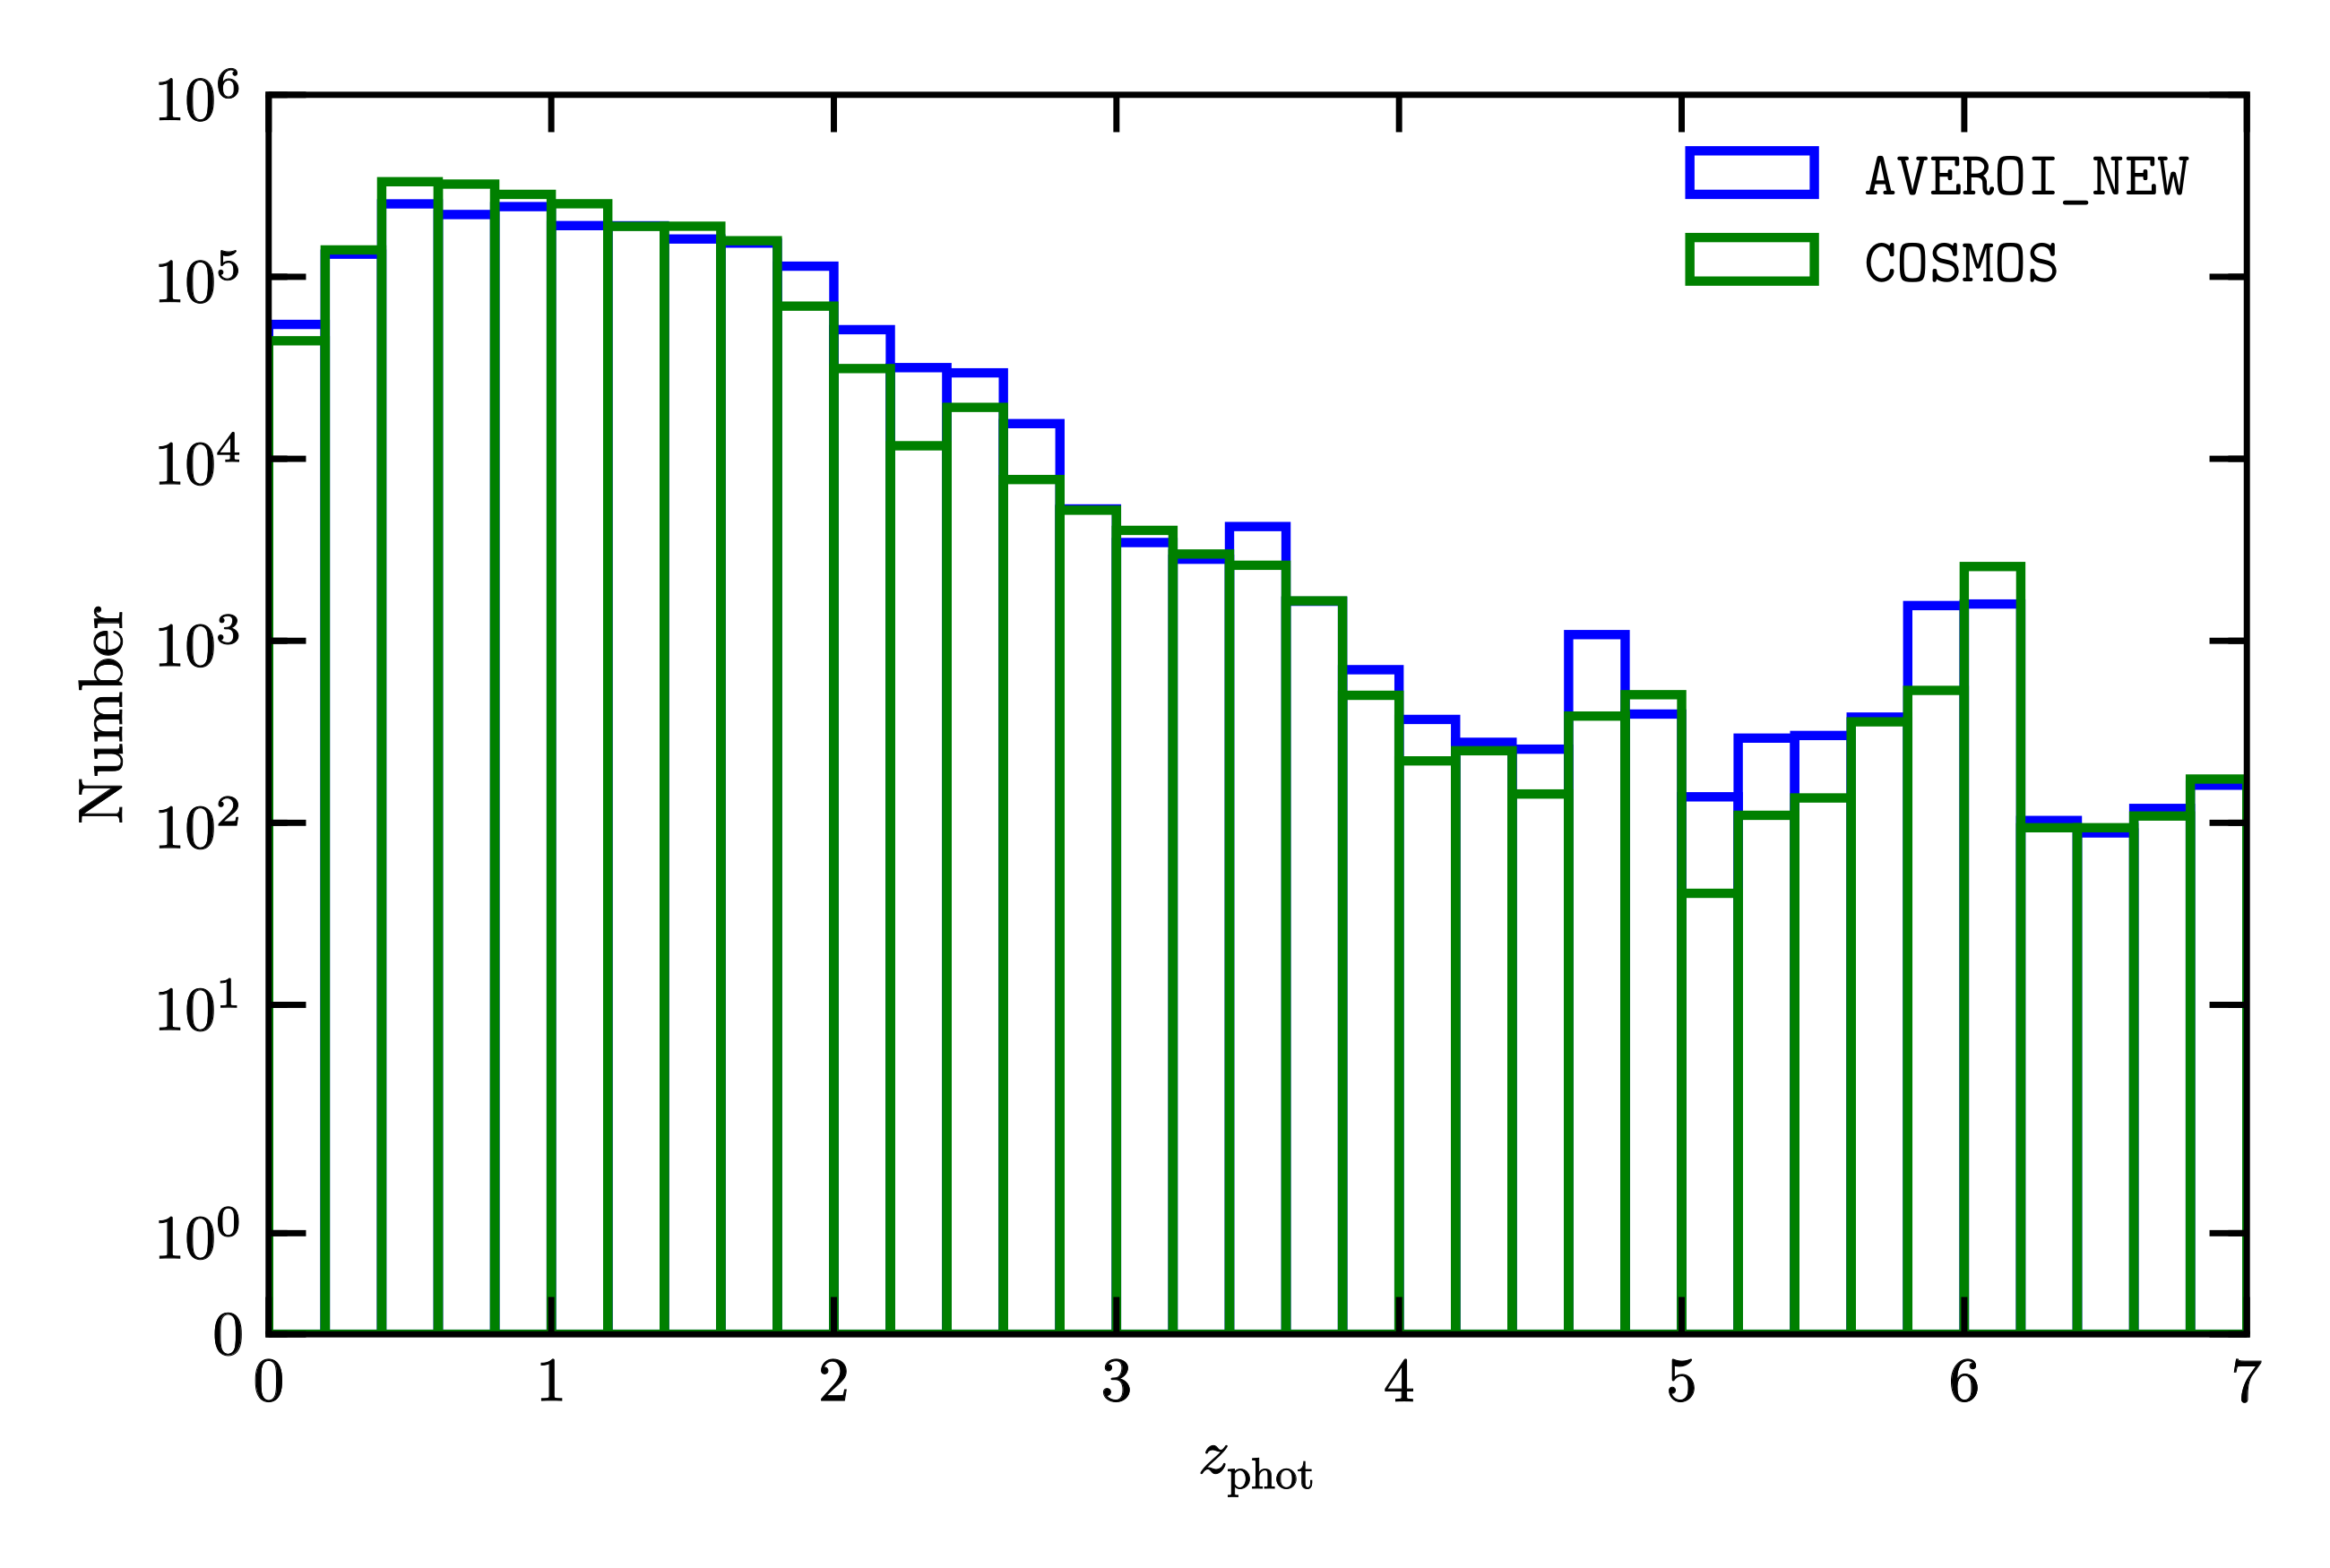
\includegraphics[width=0.95\textwidth]{photoz_distribution_combined.png}
\caption[Total photometric redshift distribution]{Photometric redshift distributions for all galaxies with good photometry in the final \DESVIDEO catalogue, plotted in bins of $\delta z=0.2$. The blue and green histograms show the photo-zs for the \texttt{AVEROI\_NEW} and \texttt{COSMOS} templates respectively. The plot exclusively includes objects classified as galaxies, selected by applying the star-galaxy separation strategy from Section \ref{subsubsection:chi_method} to the $\chi^2_{\nu,\mathrm{gal}}$ output from the respective template sets. Sources with unreliable photometry have been removed via their \texttt{FLAGS\_WEIGHT} values as described in the text.}
\label{fig:photoz_distribution_total}
\end{figure*}


Figure \ref{fig:photoz_distribution_total} presents the redshift distribution of all the selected galaxies with good photometry, showing the results for both template sets. To reduce the chances of unreliable photometry causing inaccurate photo-zs, sources with non-zero \texttt{FLAGS\_WEIGHT} values have been removed from the plot (using the same procedure as before in Sections \ref{section:photoz_computation} and \ref{subsubsection:star_galaxy_validation}), leaving \num{1919510} galaxies for \texttt{AVEROI\_NEW} and \num{2129053} for \texttt{COSMOS}. The histograms show that the two configurations produce a broadly similar distribution, with several noteworthy peaks at high redshifts. These features originate from transitions between filters, and correspond to changes in the dropout bands of Lyman-break galaxies. For instance, the strong peak at $z_{\mathrm{phot}}\equiv6$ is situated around the $z_{\mathrm{phot}}=5.99$ point where $r$-dropouts end and $i$-dropouts begin. The similar behaviour around $z\equiv4.8$ is caused by the changeover between $g$-dropouts and $r$-dropouts at $z_{\mathrm{phot}}=4.84$. The prior is likely to be a contributing factor as to why galaxies tend to cluster around these peaks; because this weighting factor leads \texttt{LePHARE} to favour the lowest redshift solution that still provides a good fit, it will tend to push the photo-z to the lowest allowable value. For Lyman-break galaxies, this lowest value is dictated by the dropout bands (e.g. for an $i$-dropout, solutions below $z_{\mathrm{phot}}=5.99$ are not compatible with the observed lack of $i$-band flux). Another contributing factor to the feature at $z\equiv6$ in particular consists of (transient) contaminants that are only observed in the $z$-band, and thus partly mimic the Lyman-break behaviour of an $i$-dropout. Section \ref{subsubsection:contamination_transients} will discuss such objects in detail. \par


The final galaxy photo-z distribution in Figure \ref{fig:photoz_distribution_total} concludes the photometric redshift part of this thesis. Equipped with all the necessary photo-z fitting data, the \DESVIDEO catalogue is ready for the selection of high-redshift galaxies, which is the topic of the next chapter.\par


